%%%%%%%%%%%%%%%%%%%%%%%%%%%%%%%%%%%%%%%%%%%%%%%%%%%%%%%%%%%%%
% This document can be formatted only with pdflatex.
%%%%%%%%%%%%%%%%%%%%%%%%%%%%%%%%%%%%%%%%%%%%%%%%%%%%%%%%%%%%%

\pdfminorversion=7
\documentclass[12pt,twoside,a4paper]{report}
\usepackage[hyphens]{url}
\usepackage{hyperref}

\usepackage[T1]{fontenc}
\usepackage[utf8]{inputenc}
\usepackage{ae}
\usepackage[pdftex]{graphicx}


\usepackage{../mondo/mondo}

\usepackage[english]{babel}
\usepackage{latexsym,epsf,epsfig}
\usepackage{rotating,amsmath,amsfonts,amssymb}

\usepackage{times}

\usepackage{listings}
\usepackage{longtable}
\usepackage{datetime}
\usepackage{xcolor}
\usepackage{tabularx}
\usepackage{tikz}
\usetikzlibrary{positioning}
\usetikzlibrary{arrows}
\usetikzlibrary{shapes.geometric}
\usepackage{amsfonts}
\usepackage{xcolor,colortbl}
\usepackage{caption}
\usepackage{subcaption}
\usepackage{pifont}
%\usepackage{adjustbox}
\usepackage{tabu}
\usepackage{multirow}
\usepackage{mathastext}

\newlength{\hsbw}
\newcommand{\comment}[1]{\mbox{}\par\vspace{0.25in}%
\setlength{\hsbw}{\linewidth}%
\addtolength{\hsbw}{-2\fboxsep}%
\addtolength{\hsbw}{-2\fboxrule}%
\noindent\fbox{\parbox{\hsbw}{{\bf Comment: }#1}}\vspace{0.25in}}
% comment-out next line to see Comments
%\renewcommand{\comment}[1]{}

% Common abbrev. are set as commands to ensure proper spacing after the dot
\newcommand{\ie}{i.e.\ \@\xspace}
\newcommand{\Ie}{i.e.\ \@\xspace}
\newcommand{\eg}{e.g.\@\xspace}
\newcommand{\Eg}{E.g.\@\xspace}
\newcommand{\etal}{et al.\@\xspace}
\newcommand{\etc}{etc.\@\xspace}

\sloppy

%%%%%%%%%%%%%%%%%%%%%%%%%%%%%%%%%%%%%%%%%%%%%%%%%%%%%%%%%%%%%%%%%%%%%
% Change title and other document information here.                 %
%%%%%%%%%%%%%%%%%%%%%%%%%%%%%%%%%%%%%%%%%%%%%%%%%%%%%%%%%%%%%%%%%%%%%

\newcommand{\didentifier}{TR}
\newcommand{\dtitle}{Train Benchmark}
\newcommand{\dversion}{1.0}
\newcommand{\dauthors}{BME}

% \dstatus should be Draft or Final %%%%%%%%%%%%%%%%%%%%%%%%%%%%%%%%%
\newcommand{\dstatus}{Draft}

% \ddist should be Partners Only, EC or Public %%%%%%%%%%%%%%%%%%%%%%%%%%%%
\newcommand{\ddist}{Public}

\newdateformat{eudate}{\THEDAY~\monthname[\THEMONTH]~\THEYEAR}
\newcommand{\ddate}{\eudate \today}
%Use a fixed date as below for final version
%\newcommand{\ddate}{24 February 2014}
\newcommand{\dyear}{2014\xspace}

%% local changes start %%

\usepackage{booktabs}
\usepackage{dcolumn}

\usepackage{amsthm}

\newcommand{\cc}[1]{\multicolumn{1}{c}{#1}}
\newcolumntype{d}[1]{D{.}{.}{#1}}
\newcommand{\code}[1]{{\texttt{#1}}}
\newcommand{\codefoot}[1]{{\texttt{#1}}}
\newcommand{\abs}[1]{|{#1}|}

% this command reduces the size of the sans-serif font so it is in level with the serif font
\renewcommand{\textsf}[1]{{\sffamily \small #1}}

\usepackage{listings}
\lstset{language=Java,basicstyle=\footnotesize,captionpos=b}

\definecolor{gray97}{gray}{.97}
\definecolor{gray75}{gray}{.75}
\definecolor{gray45}{gray}{.45}
\definecolor{gray20}{gray}{.20}

\lstdefinestyle{shell}{
  tabsize=2,
  language=,
  xleftmargin=.5cm,
  framexleftmargin=.4cm,
  keywordstyle=\color{gray20},
  breaklines=true,
  captionpos=t,
  basicstyle=\ttfamily\small,
  showstringspaces=false,
  numberstyle=\ttfamily\tiny,
  numbersep=1.1cm,
  numbers=left,
  numbersep=5pt,
  frameround=ftff,
  showspaces=false,
  showtabs=false,
  frame=single,
  backgroundcolor=\color{gray97},
  rulesepcolor=\color{black},
  commentstyle=\color{gray45}
}

\newcommand{\tuple}[1]{\langle #1 \rangle}

\newcommand{\picScale}[3]{
	\begin{figure}[!htb]
		\centering
		\includegraphics[scale=#3]{figures/#1}
		\caption{#2}
		\label{fig:#1}
	\end{figure}}

\newcommand{\picCustom}[3]{
	\begin{figure}[!htb]
		\centering
		\begin{adjustbox}{max size={#3\textwidth}{\textheight}}
			\includegraphics[scale=1.0]{figures/#1}
		\end{adjustbox}
		\caption{#2}
		\label{fig:#1}
	\end{figure}}

\newcommand{\picBig}[2]{\picCustom{#1}{#2}{1.3}}
\newcommand{\pic}[2]{\picCustom{#1}{#2}{1.0}}
\newcommand{\picSmall}[2]{\picCustom{#1}{#2}{0.8}}
\newcommand{\picTiny}[2]{\picCustom{#1}{#2}{0.6}}

\newcommand{\tb}{Train Benchmark}

\newcommand{\union}{\cup}
\newcommand{\intersection}{\cap}
\newcommand{\parentheses}[1]{\left(#1\right)}
\newcommand{\op}[2]{\mathrm{#1}\parentheses{#2}}
\newcommand{\deltadifference}[1]{\parentheses{#1 \setminus \Delta #1}}
\newcommand{\deltaunion}[1]{\parentheses{#1 \union \Delta #1}}
\newcommand{\consequence}{\quad \Rightarrow \quad}
\newcommand{\figref}[1]{\autoref{fig:#1}}
\newcommand{\lstref}[1]{\autoref{lst:#1}}
\newcommand{\naturaljoin}{\bowtie}
\newcommand{\antijoin}{\, \triangleright \,}


\definecolor{listinggray}{rgb}{0.9,0.9,0.9}
\definecolor{keywordcolor}{rgb}{0.5,0,0.1}
\definecolor{commentcolor}{rgb}{0,0.3,0.1}
\definecolor{stringcolor}{rgb}{0,0,1}
\lstset{backgroundcolor=\color{listinggray}}
\lstset{basicstyle=\scriptsize\ttfamily}
\lstset{commentstyle=\itshape\color{commentcolor}\ttfamily}
\lstset{stringstyle=\color{stringcolor}\ttfamily}
\lstset{frameround=tttt}
\lstset{captionpos=b}
\lstset{keywordstyle=\color{keywordcolor}\bfseries\ttfamily}
\lstset{showstringspaces=false}
\lstset{tabsize=2}
\lstset{numbers=left,numberstyle=\scriptsize\ttfamily,stepnumber=1,numbersep=5pt}
\lstset{escapeinside={(*@}{@*)}}

\lstdefinelanguage{iqpl}
{morekeywords={@Interpretation,@Trigger,count,sum,max,min,avg,shareable,trigger,guard,eval,
asmfunction,rule,gtrule,if,do,choose,forall,iterate,print,println,log,apply,
    entity,relation,supertypeOf,subtypeOf,typeOf,instanceOf,try,else,pattern,
    precondition,postcondition,action,neg,find,import,namespace,in,below,out,
    inout,let,multiplicity,many_to_one,many_to_many,one_to_many,one_to_one,
    isAggregation,inverse,seq,update,ref,true,false,call,machine,or,
    undef,rename,new,del,delete,move,copy,value,setValue,setFrom,setTo,with,when,check,change,appear,disappear,cdrule,transformation,common,from,to,toInteger},
 sensitive=true, morecomment=[l]{//}, morecomment=[s]{/*}{*/},
 morestring=[b]{"},
}
\newcommand{\sourceIQPL}[1]
{
\lstset{
backgroundcolor=\color{listinggray},
basicstyle=\scriptsize\ttfamily,
commentstyle=\itshape\color{commentcolor}\ttfamily,
stringstyle=\color{stringcolor}\ttfamily,
frameround=tttt,
captionpos=b,
keywordstyle=\color{keywordcolor}\bfseries\ttfamily,
showstringspaces=false,
tabsize=2,
numbers=left,numberstyle=\scriptsize\ttfamily,stepnumber=1,numbersep=5pt,
language=iqpl,
escapeinside={(*@}{@*)}
}

\lstinputlisting{#1}
}

\newcommand{\sourceDRL}[1]
{
\lstset{
morekeywords={query, end, package, not, memberOf, contains},
sensitive=true, morecomment=[l]{//}, morecomment=[s]{/*}{*/},
morestring=[b]{"},
backgroundcolor=\color{listinggray},
basicstyle=\scriptsize\ttfamily,
commentstyle=\itshape\color{commentcolor}\ttfamily,
stringstyle=\color{stringcolor}\ttfamily,
frameround=tttt,
captionpos=b,
keywordstyle=\color{keywordcolor}\bfseries\ttfamily,
showstringspaces=false,
tabsize=2,
numbers=left,numberstyle=\scriptsize\ttfamily,stepnumber=1,numbersep=5pt,
escapeinside={(*@}{@*)}
}

\lstinputlisting{#1}
}

\newcommand{\sourceOCL}[1]
{
\lstset{
morekeywords={invariant, and, or, implies, not, oclIsKindOf, self, forAll, exists, oclAsType, includes, allInstances},
sensitive=true, morecomment=[l]{//}, morecomment=[s]{/*}{*/},
morestring=[b]{"},
backgroundcolor=\color{listinggray},
basicstyle=\scriptsize\ttfamily,
commentstyle=\itshape\color{commentcolor}\ttfamily,
stringstyle=\color{stringcolor}\ttfamily,
frameround=tttt,
captionpos=b,
keywordstyle=\color{keywordcolor}\bfseries\ttfamily,
showstringspaces=false,
tabsize=2,
numbers=left,numberstyle=\scriptsize\ttfamily,stepnumber=1,numbersep=5pt,
escapeinside={(*@}{@*)}
}

\lstinputlisting{#1}
}

\newcommand{\sourceSPARQL}[1]
{
\lstset{
morekeywords={SELECT, WHERE, OPTIONAL, FILTER, NOT, EXISTS, sameTerm, bound},
sensitive=true, morecomment=[l]{//}, morecomment=[s]{/*}{*/},
morestring=[b]{"},
backgroundcolor=\color{listinggray},
basicstyle=\scriptsize\ttfamily,
commentstyle=\itshape\color{commentcolor}\ttfamily,
stringstyle=\color{stringcolor}\ttfamily,
frameround=tttt,
captionpos=b,
keywordstyle=\color{keywordcolor}\bfseries\ttfamily,
showstringspaces=false,
tabsize=2,
numbers=left,numberstyle=\scriptsize\ttfamily,stepnumber=1,numbersep=5pt,
escapeinside={(*@}{@*)}
}

\lstinputlisting{#1}
}

\newcommand{\sourceJava}[1]
{
\lstset{
language=java,
backgroundcolor=\color{listinggray},
basicstyle=\scriptsize\ttfamily,
commentstyle=\itshape\color{commentcolor}\ttfamily,
stringstyle=\color{stringcolor}\ttfamily,
frameround=tttt,
captionpos=b,
keywordstyle=\color{keywordcolor}\bfseries\ttfamily,
showstringspaces=false,
tabsize=2,
numbers=left,numberstyle=\scriptsize\ttfamily,stepnumber=1,numbersep=5pt,
escapeinside={(*@}{@*)}
}
\lstinputlisting{#1}
}

\newcommand{\sourceRDF}[1]
{
\lstset{
morekeywords={prefix},
sensitive=true, morecomment=[l]{//}, morecomment=[s]{/*}{*/},
morestring=[b]{"},
backgroundcolor=\color{listinggray},
basicstyle=\scriptsize\ttfamily,
commentstyle=\itshape\color{commentcolor}\ttfamily,
stringstyle=\color{stringcolor}\ttfamily,
frameround=tttt,
captionpos=b,
keywordstyle=\color{keywordcolor}\bfseries\ttfamily,
showstringspaces=false,
tabsize=2,
numbers=left,numberstyle=\scriptsize\ttfamily,stepnumber=1,numbersep=5pt,
escapeinside={(*@}{@*)}
}
\lstinputlisting{#1}
}

\newcommand{\alignListing}{\lstset{xleftmargin=5mm, framexleftmargin=5mm, numbers=left}}

%\lstset{keepspaces=true}
\lstset{basicstyle=\ttfamily\upshape}
\lstset{flexiblecolumns=true}
\lstdefinelanguage{viatra} {morekeywords={@Trigger,
trigger,asmfunction,rule,gtrule,if,do,choose,forall,iterate,print,println,log,apply,
    entity,relation,supertypeOf,subtypeOf,typeOf,instanceOf,try,else,pattern,
    precondition,postcondition,action,neg,find,import,namespace,in,below,out,
    inout,let,multiplicity,many_to_one,many_to_many,one_to_many,one_to_one,
    isAggregation,inverse,seq,update,ref,true,false,call,machine,or,
    undef,rename,new,del,delete,move,copy,setValue,setFrom,setTo,with,
    then},
 sensitive=true,
 morecomment=[l]{//},
 morecomment=[s]{/*}{*/},
 morestring=[b]{"},
}

%\lstset{backgroundcolor=\color{listinggray}}
\lstset{basicstyle=\scriptsize\ttfamily}
\lstset{commentstyle=\itshape\ttfamily}
\lstset{stringstyle=\ttfamily}
\lstset{frameround=tttt} \lstset{captionpos=b}
\lstset{keywordstyle=\bfseries\ttfamily}
\lstset{showstringspaces=false}
\lstset{escapeinside={(*@}{@*)}}
\lstset{language=viatra}


\lstnewenvironment{Java} {\lstset{
  basicstyle=\fontsize{8}{10}\ttfamily,xleftmargin=12pt,
  language=Java,
  columns=flexible, % add any modifications here
}}{}

\newtheorem{lemma}{Lemma}
\newtheorem{theorem}{Theorem}
\newtheorem{criterion}{Criterion}
\newtheorem{definition}{Definition}

%% local changes end %%

\usepackage{multicol}
\usepackage{bytefield}
%\usepackage{colortbl}
\usepackage{textcomp}

\newcommand{\XOR}{\textasciicircum\xspace}
\newcommand{\OR}{\textbar\xspace}
\newcommand{\AND}{\&\xspace}
\newcommand{\NOT}{\texttildelow}
\newcommand{\shl}{\textless$\!$\textless\xspace}
\newcommand{\shr}{\textgreater$\!$\textgreater$\!$\textgreater\xspace}
\newcommand{\ashr}{\textgreater$\!$\textgreater\xspace}

\renewcommand{\figureautorefname}{Figure}
\renewcommand{\tableautorefname}{Table}
\renewcommand{\partautorefname}{Part}
\renewcommand{\chapterautorefname}{Chapter}
\renewcommand{\sectionautorefname}{Section}
\renewcommand{\subsectionautorefname}{Section}
\renewcommand{\subsubsectionautorefname}{Section}

\newcommand{\todo}[1]{\textbf{TODO:  }{#1}}
\newcommand{\concept}[1]{\emph{#1}\index{#1}\label{def:#1}}
\newcommand{\incquery}{\textsc{EMF-IncQuery}}
\let\codeCap\texttt

\newcommand{\benchmarkresult}[2]{
\begin{figure}[!Htb]
	\centering
	\includegraphics[width=\textwidth]{figures/benchmark-results/#1}
	\caption{#2}
	\label{fig:#1}
\end{figure}}


\begin{document}

\firstpage

\partnerpage


\newpage
\tableofcontents

\newpage
% % % % % % % % % % % % % % % % % % % % % % % % % % % % % % % % % % % % % % % %
\section*{Document Control}

\begin{tabular}{*{3}{|p{.3\textwidth}}|}\hline
\centering{\bf Version} &
\centering{\bf Status} &
\centering{\bf Date}\tabularnewline\hline
\centering{0.1} & \centering{Document outline} & \centering{27 January 2014} \tabularnewline\hline
\centering{0.4} & \centering{Preliminary draft} & \centering{28 February 2014} \tabularnewline\hline
\centering{0.99} & \centering{Tentative final draft} & \centering{28 March 2014} \tabularnewline\hline
\end{tabular}

\clearpage
\pagenumbering{arabic}

%%%%%%%%%%%%%%%%%%%%%%%%%%%%%%%%%%%%%%%%%%%%%%%%%%%%%%%%%%%%
\chapter*{Executive Summary}
The main goal of the Train Benchmark is to measure the \emph{execution time} of graph-based query processing tools with particular emphasis on incremental query reevaluation. The execution time is measured against models of growing sizes generated by an instance model generator. This way, the scalability of the tools is evaluated. The Train Benchmark also demonstrates other abilities of the tools, including transformation capabilities, conciseness of the query and transformation language, convenience of the API, compatibility with different metamodeling languages and so on. The Train Benchmark is a general benchmarking framework, that contains a specific benchmark test case set built around a metamodel inspired by railway system design. This test case set also comes with a set of queries and transformation operations. 

The current tech report includes information on two variants of the Train Benchmark: the original version was described in~\cite{SCP2014} and describes the incremental well-formedness checking scenario. The extended version was described in~\cite{ASE2013} and introduces query and instance model query metrics to quantitatively assess the ``difficulty'' of various model query-instance model combinations to find those metrics that are best for predicting the query evaluation time without running the query itself.

The most up-to-date supplementary material is found at \url{https://opensourceprojects.eu/p/mondo/wiki/TrainBenchmark}

Scalability issues in model-driven engineering arise due to the increasing
complexity of modeling workloads. This complexity comes from two main factors:
(i) \emph{instance model sizes} are exhibiting a tremendous growth as the
complexity of systems-under-design is increasing, (ii) increasing \emph{feature
sophistication} in toolchains, such as complex model validation or
transformations.

One of the the most computationally expensive tasks in modeling applications are
\emph{model queries}. While there are a number of existing benchmarks for
queries over relational databases \cite{tpc-c} or graph stores
\cite{BerlinBenchmark, SP2Bench}, modeling tool workloads are significantly
different. Specifically, modeling tools use much more complex queries than
typical transactional systems, and the real world performance is affected by
response time (i.e. execution time for a specific operation such as validation
or transformation) than throughput (i.e. the amount of parallel transactions).


\paragraph{Overview}
To address this challenge, the Train Benchmark \cite{TB:SCP2013,TBwebsite} is a macro
benchmark that aims to measure batch and incremental query evaluation
performance, in a scenario that is specifically modeled after \emph{model
validation} in (domain-specific) modeling tools: at first, the entire model is
validated, then after each model manipulation (e.g., the deletion of a
reference) is followed by an immediate re-validation. The benchmark records
execution times for four phases:

\begin{enumerate}
 \item During the \emph{read} phase, the instance model
 is loaded from hard drive to memory. This includes the parsing of the input as
 well as initializing data structures of the tool. 
 
 \item In the \emph{check} phase, the instance model is queried to identify
 invalid elements. This can be as simple as reading the results from cache, or
 the model can be traversed based on some index. By the end of this phase,
 erroneous objects need to made available in a list.
 
 \item In the \emph{edit} phase, the model is modified to simulate effects of
 manual user edits. Here the size of the change set can be adjusted to
 correspond to small manual edits as well as large model transformations.
 
 \item The re-validation of the model is carried out in the \emph{re-check}
 phase similarly to the \emph{check} phase.
\end{enumerate}

The Train Benchmark computes two derived results based on the recorded data:
(1) \emph{batch validation time} (the sum of the \emph{read} and {check} phases)
represents the time that the user must wait to start to use the tool; (2)
\emph{incremental validation time} consists of the \emph{edit} and
\emph{re-check} phases performed $100$ times, representing the time that the
user spent waiting for the tool validation.


\paragraph{Instance models}
The Train Benchmark uses a domain-specific model of a railway system that
originates from the MOGENTES EU FP7 project, where both the metamodel and the
well-formedness rules were defined by railway domain experts. This domain
enables the definition of both simple and more complex model queries while it is
uncomplicated enough to incorporate solutions from other technological spaces
(e.g. ontologies, relational databases and RDF). This allows the comparison of
the performance aspects of wider range of query tools from a constraint
validation viewpoint.

The instance models are systematically generated based on the metamodel and the
defined complex model queries: small instance model fragments are generated
based on the queries, and then they are placed, randomized and connected to each
other. The methodology takes care of controlling the number of matches of all
defined model queries. To break symmetry, the exact number of elements and
cardinalities are randomized.
 
This brings artificially generated models \emph{closer to real world instances},
and \emph{prevents query tools from efficiently storing} or caching of instance
models. During the generation of the railway system model, errors are injected
at random positions. These errors can be found in the check phase of the
benchmark, which are reported, and can be corrected during the edit phase. The
initial number of constraint violating elements are low (<1\% of total
elements).
 
\paragraph{Queries and transformations}
Queries are defined informally in plain text (in a tool independent way) and
also formalized using the standard OCL language as a reference implementation
(available on the benchmark website \cite{TBwebsite}). The queries range from
simple attribute value checks to complex navigation operations consisting of
several (4+) joins.

The functionally equivalent variants of these queries are formalized using the
query language of different tools applying tool based optimizations. As a
result, all query implementations must return (the same set of) invalid instance
model elements.
 
In the \emph{edit} phase, the model is modified to change the result set to be
returned by the query in the re-check phase. For simulating manual
modifications, the benchmark always performs hundred random edits (fixed low
constant) which increases the number of erroneous elements. An edit operation
only modify single model elements at once - more complex model manipulation is
modelled as a series of edits.

\paragraph{Evaluation of measurements}
The Train Benchmark defines a Java-based framework and application programming
interface that enables the integration of additional metamodels, instance
models, query implementations and even new benchmark scenarios (that may be
different from the original 4-phase concept). The default implementation
contains a benchmark suite for queries implemented in Java, Eclipse OCL and
EMF-IncQuery.

Measurements are recorded automatically in a machine-processable format (CSV)
that is automatically processed by R \cite{TB:R} scripts. An extended version of the Train
Benchmark \cite{TB:ASE2013} features several (instance model, query-specific and
combined) \emph{metrics} that can be used to characterize the ``difficulty'' of
benchmark cases numerically, and -- since they can be evaluated automatically
for other domain/model/query combinations -- allow to compare the benchmark
cases with other real-world workloads.

%%----------------------------------------------------------------------------
\chapter*{Introduction}\addcontentsline{toc}{chapter}{\bevezeto}
%----------------------------------------------------------------------------

% Queries in MDE: scalability challenge
Nowadays, model-driven software engineering (MDSE) plays an important role in the development processes of critical embedded systems. Advanced modeling tools provide support for a wide range of development tasks such as requirements and traceability management, system modeling, early design validation, automated code generation, model-based testing and other validation and verification tasks. With the dramatic increase in complexity that is also affecting critical embedded systems in recent years, modeling toolchains are facing scalability challenges as the size of design models constantly increases, and automated tool features become more sophisticated.

% Techniques to achieve scalability
A key factor in the scalability of MDE toolchains is the performance of model representation~\cite{GrandChallengeScalability}, which is, in turn, determined by the characteristics of persistence, query evaluation and model manipulation operations. Traditionally, modeling tools built on state-of-the-art frameworks such as the Eclipse Modeling Framework (EMF~\cite{EMF}) have relied on an in-memory object model backed by an XML serialization. More recently, \emph{model repositories} (such as CDO~\cite{CDO} or Morsa~\cite{COLLAB:MORSA}) have emerged that aim to tackle scalability issues by making use of advances in object persistence technology. As the majority of model-based tools uses a graph-oriented data model, recent results of the NoSQL and Linked Data movement~\cite{neo4j,openvirtuoso,sesame} are straightforward candidates for adaptation to MDE purposes. 

\emph{Model queries} support several essential scenarios including model validation, model transformations, model synchronization, view maintenance and model execution. As a consequence, many scalability issues can be addressed by improving query performance. This led to the development of several model indexing and query evaluation engines (such as Eclipse OCL~\cite{EclipseOCL}, EMF Query~\cite{EMF:ModelQuery}, complementary approaches that translate model queries into lower level queries that can be executed on the (relational) back-end~\cite{scheidgen2012automated}). 
There are also several approaches (such as \mbox{\textsc{EMF-IncQuery}}~\cite{models10} and the Impact Analyzer of Eclipse OCL~\cite{EclipseOCL}) to support the \emph{incremental evaluation} of model queries, which reduces query response time by limiting the impact of model modifications to query result calculation.

% Benchmarks
For tool engineers, \emph{benchmarks} may provide guidance on picking the right technology for building a new tool architecture to fulfill increasing scalability requirements. Due to their central role in data-intensive applications, the performance of persistence technologies has been evaluated by many benchmarks~\cite{BSBM,SP2Bench} % TODO cite
that focus on throughput and response time measurements, and investigate scalability in terms of the size of the data set and the number of transactions. In addition to these traditional scalability aspects, the semantic web community has investigated the scalability of semantic graph databases (RDF triple stores). These benchmarks rely on graph queries over a structurally richer data set and also investigate the effects of advanced semantic technologies such as inference. Up to now, the most complex benchmarking workloads have been investigated by the academic and industrial MDE tool building community in transformation tool contests~\cite{TTC}, which feature synthetic model transformation case studies inspired by real-world applications.

% Challenges: lack of predictability, and generalizability to actual MDSE workloads
% key differences
Despite all these efforts, \emph{making a well-founded technological choice} based on existing benchmarking results \emph{remains a tough challenge}. First, MDE tools have very specific \emph{workloads} (both in terms of model structure and transaction complexity) \emph{that are different} in key aspects compared to traditional RDBMS and newer graph persistence benchmarks. MDE tools rely on much more complex queries and their performance is dominated by response time and re-evaluation time rather than throughput. Additionally, RDBMS and semantic technologies have key conceptual differences that require mapping layers which might have adverse and unpredictable effects on real life performance.
The generalizability of benchmark results is further limited by the \emph{scarcity of relevant metrics} that could be used to assess an engineering problem and predict which technology would be best suited. Existing metrics emphasize a single aspect of the problem (most typically model size), while internal metrics (used by e.g. optimizing query evaluation engines or pattern matchers inside GT tools, for estimating query evaluation difficulty) are either not documented well or not accessible in a reusable way.


In this paper, we aim to address these challenges by \emph{assessing existing metrics, along with newly proposed ones}. These metrics take instance model characteristics, static query characteristics and their combination into account. Based on our real-life experiences with tools and models, we \emph{outline a benchmark} that uses model validation as its core scenario, thus focusing on model loading and model validation workloads. Guidelines are provided on the generation of instance models and queries, on which we evaluated the metrics and executed the benchmark using three, characteristically different graph query tools. In order to identify which metrics provide reliable performance prediction for a given workload and tool category, we \emph{calculate the correlation with significance values} between execution times and metrics.

% % proposal: metrics for estimation, benchmark for differentiation 
% In this paper, we aim to address these challenges by \emph{assessing (existing and novel) metrics} that take instance model characteristics, static query characteristics and their combination %of both query and instance model characteristics 
% into account. 
% By providing guidelines on instance model generation and case study fine tuning to achieve result dispersion (to provide differentiation between various technologies), we outline a benchmark that uses model validation as the core scenario.
% Our experimental measurements evaluate the metrics over the test set of our benchmark over  three characteristically different classes of query technologies. We calculate the correlation of the predictions provided by the metrics with the measurement data to highlight which metrics provide reliable prediction for a certain query technology.
% %with results to identity those metrics that can reliably predict application performance.

% Structure
The rest of the paper is structured as follows. 
\autoref{sec:background} overviews the most important concepts of modeling languages and model queries, and 
\autoref{sec:relwork} discusses benchmarking and metrics related work.
\autoref{sec:benchmark} presents our analysis of existing benchmarks and proposes new metrics and benchmarks, with their evaluation presented in \autoref{sec:eval}.
\autoref{sec:conclusion} outlines directions for future work and concludes the paper.

\chapter{Train Benchmark Technical Specification}

This chapter discusses the technical specification of the Train Benchmark. In order to ensure fair comparison of different tools, the specification describes the queries, transformations and the instance model generator in detail. The phases in the benchmark are also strictly defined.

Currently, the Train Benchmark comes in two versions: the original version (\autoref{specification-original}) and an extended version (\autoref{specification-extended}), first discussed in paper~\cite{ASE2013}.
 
\section{Original Version}
\label{specification-original}

A \concept{test case} configuration for every tool consists of an \emph{instance model} (\autoref{sec:instanceGeneration}) with an \emph{instance model size}, a \emph{predefined query} (\autoref{sec:queries}) describing constraint violating elements and the name of the \emph{scenario} (\autoref{sec:scenarios}) to run.

As a result of a testcase run, the \emph{execution times} of each phase, the \emph{memory usage} and the \emph{number of erroneous elements} are measured and recorded. The number of invalid elements are used to check the correctness of the validation, however the set of element identifiers must also be available for later processing. 


\subsection{Phases}
\label{sec:phases}

\begin{figure}[htb]
	\centering
	%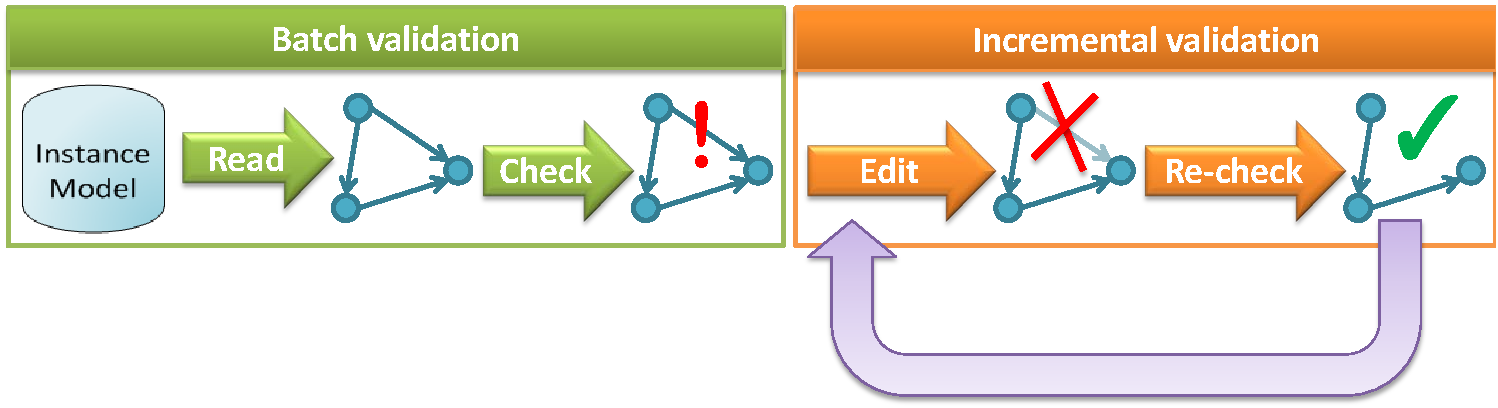
\includegraphics[scale=0.5]{figures/phases}
	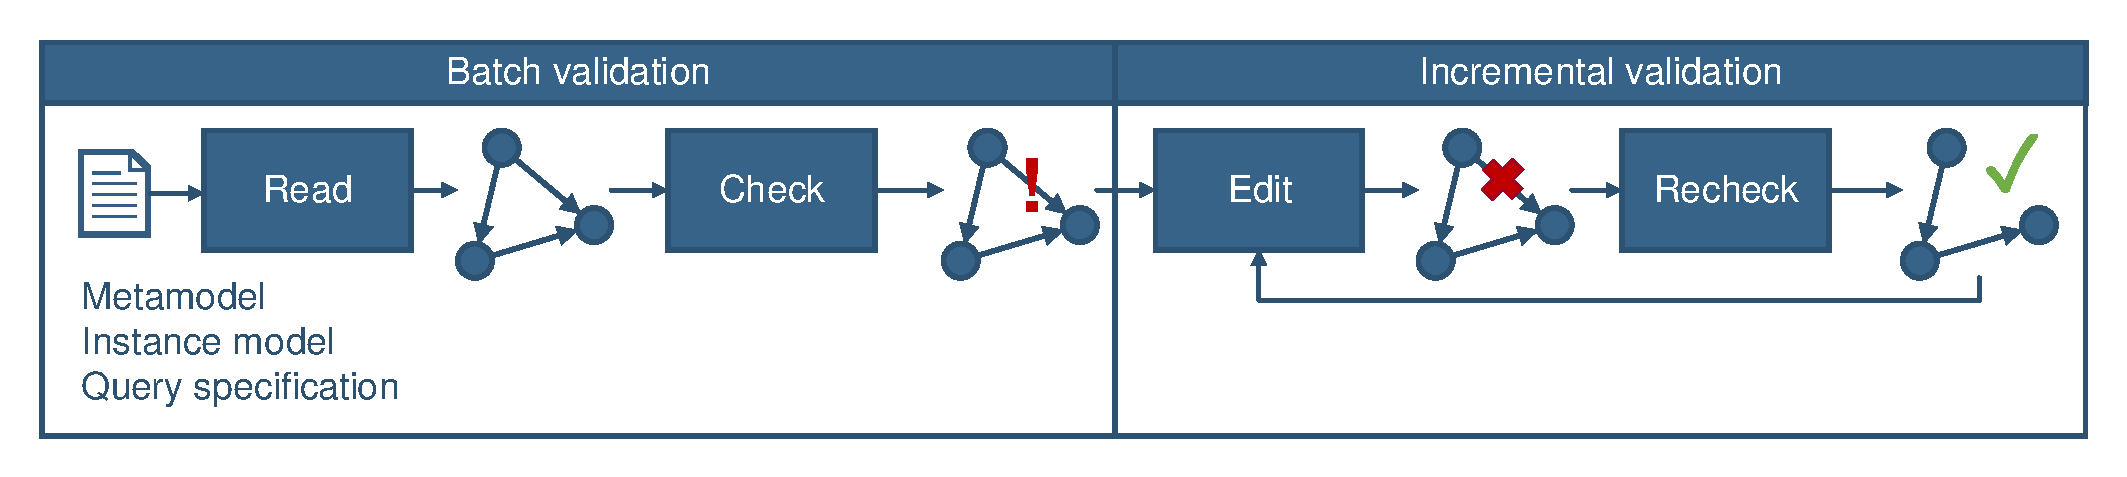
\includegraphics[width=\textwidth]{figures/trainbenchmark-sequence}
	\caption{The phases of the benchmark.}
	\label{fig:phases}
\end{figure}

To measure performance for re-validating a model after modifications, four benchmark \concept{phases} were defined, as illustrated in \figref{fig:phases}.
\begin{enumerate}
 
 \item During the \concept{read} phase, the previously generated instance model and validation query are loaded from hard drive to memory. This includes the parsing of the input as well as initializing data structures of the tool.
 
 \item In the \concept{check} phase, the instance model is queried to identify invalid elements. This can be as simple as reading the results from cache, or the model can be traversed based on some index. By the end of this phase, erroneous objects need to made available in a collection for further processing.
 
 \item In the \concept{edit} phase, the model is changed to simulate effects (and measure performance) of model modifying operations. At the beginning of this phase ``query-like'' functions are used to gather elements to be modified, however this time is excluded, and only the required time of model editing operations are recorded in this phase. (As query performance is measured in the check phases.)
 
 \item The re-validation of the model is carried out in the \concept{re-check} phase similarly to the \emph{check} phase.
\end{enumerate}

\subsection{Use Case Scenarios of the Benchmark}
\label{sec:scenarios}

Paper~\cite{icgt08-bhrv} analyzes performance of algorithms used for graph
pattern query evaluation and identifies two use cases where efficient
\emph{incremental model validation} is required. The batch part of our benchmark
consists of the execution of the read and first check phases. Inspired by paper
\cite{icgt08-bhrv}, three \concept{scenarios} were defined to measure different
use cases:
\begin{itemize}
  
  \item \concept{Batch validation scenario} (\textsf{Batch}):
  In this scenario the model is \emph{read} in one batch from storage, than a model validation is carried out by executing the query in the check phase. Such use case is performed when a model editor is opened and initial validations are issued by the designer. 
  
  \item \concept{Fault injection scenario} (\textsf{Inject}):
  The fault injection scenario extends the batch validation scenario by differential model modification and re-checking phases. After the batch validation a small model manipulation step is performed (\eg a reference is deleted), which is immediately followed by re-validation to get instantaneous feedback.  In this scenario such small edit and re-check phases are executed in sequence.
  
  Such scenario occurs when someone uses a typical UML editor (for designing software solutions), or a domain-specific editor where elements or relations are added one-by-one. These editors should detect design errors quickly and early in the development process to let engineers refine models and cut down debugging and error correction costs.
  
  \item \concept{Automated model repair scenario} (\textsf{Repair}):
  The automated model repair scenario extends the batch validation scenario by differential model modification and re-checking phases. In the edit phase, the model is repaired, based on the erroneous objects identified during the batch validation. This is carried out by the tool itself performing mass edits automatically. Finally, the whole model is re-checked, and remaining or newly introduced errors are reported. 
  
  Efficient execution of such a use case is necessary during refactoring, incremental code generation, or when a model is transformed from a source language to a target language by a model transformation program, using model synchronisation.

\end{itemize}


\subsection{Metamodel}
\label{sec:domain}

\begin{figure}
	\centering
	\begin{subfigure}[b]{\textwidth}
		\centering
		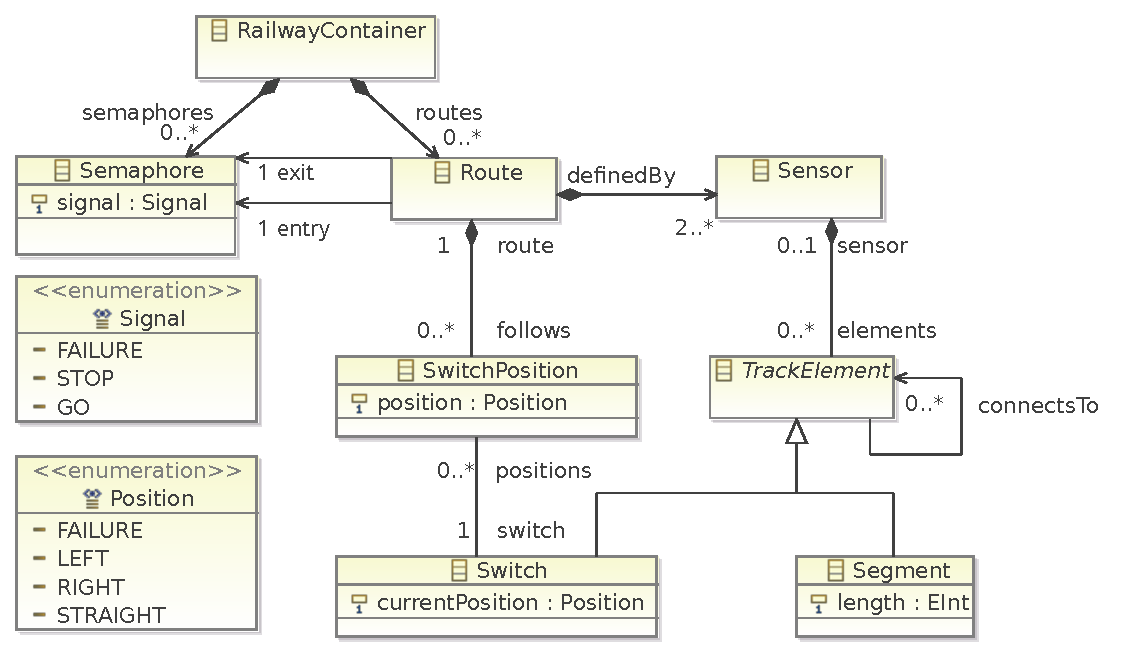
\includegraphics[scale=0.6]{figures/railway-containments}
		\caption{Containment hierarchy and references}
		\label{fig:railway-containments}
	\end{subfigure}
	~
	\begin{subfigure}[b]{\textwidth}
		\centering
		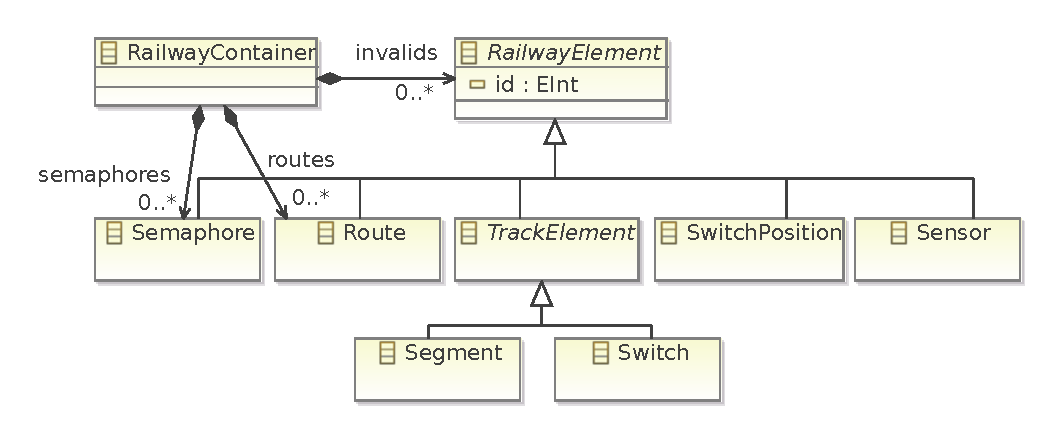
\includegraphics[scale=0.6]{figures/railway-inheritance}
		\caption{Supertype relations}
		\label{fig:railway-inheritance}
	\end{subfigure}
	\caption{The metamodel of the Train Benchmark.}
	\label{fig:metamodel}
\end{figure}

The metamodel of the railway domain used in the Train Benchmark is depicted in \figref{fig:metamodel}. A train \textsf{route} can be defined by a set of \textsf{sensors}. Sensors are associated with \textsf{track elements}: track \textsf{segment}s (with a specific length) or \textsf{switch}es. A route may have associated \textsf{switch positions} which describe the required state of a switch belonging to the route. Different route definitions can specify different states for a specific switch.
 
\subsection{Queries}
\label{sec:queries}

In the validation and re-validation phases of the benchmark, the queries return the elements violating the well-formedness constraint defined by the test case. These constraints are first defined informally in plain text and then formalized using a query language suited for the benchmarked tool. As a result, the query must return a set of the invalid instance model elements' identifiers.
 
Two simple queries involving maximum 2 objects (\textsf{PosLength} and \textsf{SwitchSensor}) and two complex queries involving 4--8 objects and multiple join operations (\textsf{RouteSensor} and \textsf{SemaphoreNeighbor}) were defined. Simple queries are able to quickly distinguish efficient tools from inefficient ones, while complex queries are used to differentiate faster model query technologies.
 
In the following, we present the queries defined in the \tb{}. We describe the semantics and the goal of each query. We also show the associated graph pattern and relational algebra query.

\subsubsection{Relational Schemas}

For formulating the queries in relational algebra we define the following relational schemas for representing the vertices (objects) in the graph (instance model).

\begin{itemize}
  \item $ \mathit{Route}\left(\mathit{id}\right) $
  \item $ \mathit{Sensor}\left(\mathit{id}, \mathit{length}\right) $
  \item $ \mathit{Semaphore}\left(\mathit{id}, \mathit{signal}\right) $
  \item $ \mathit{Switch}\left(\mathit{id}, \mathit{currentPosition}\right) $
  \item $ \mathit{SwitchPosition}\left(\mathit{id}, \mathit{position}\right) $
  \item $ \mathit{TrackElement}\left(\mathit{id}\right) $
\end{itemize}

The edges\footnote{also called relationships or references in various implementations} are represented with the following relational schemas:

\begin{itemize}
  \item $ \mathit{entry}\left(\mathit{Route}, \mathit{Semaphore}\right) $
  \item $ \mathit{exit}\left(\mathit{Route}, \mathit{Semaphore}\right) $
  \item $ \mathit{follows}\left(\mathit{Route}, \mathit{SwitchPosition}\right) $
  \item $ \mathit{definedBy}\left(\mathit{Route}, \mathit{Sensor}\right) $
  \item $ \mathit{switch}\left(\mathit{SwitchPosition}, \mathit{Switch}\right) $
  \item $ \mathit{sensor}\left(\mathit{Switch}, \mathit{Sensor}\right) $
  \item $ \mathit{connectsTo}\left(\mathit{TrackElement}_1, \mathit{TrackElement}_2\right) $
\end{itemize}

\subsubsection{Graph Patterns}

In the following, we represent the graph pattern representation for the violation of each well-formedness constraint. For defining the patterns and transformations, we used a graphical syntax similar to GROOVE~\cite{rensink2004groove} with a couple of additions:

\begin{itemize}
  \item The invalid model elements returned by the query are shown in \textbf{bold} font.
  \item Filter conditions are shown in \textit{italic} font.
  \item Negative application conditions are shown with in a \textcolor{negcolor}{red} rectangle with the \textcolor{negcolor}{\textsf{NEG}} caption.
  \item The insertions are with a \textcolor{newcolor}{\guillemotleft{}new\guillemotright{}} caption, while deletions are marked with a \textcolor{delcolor}{\guillemotleft{}del\guillemotright{}} caption. Attribute updates are also show in \textcolor{newcolor}{green}.
\end{itemize}

%%%%%%%%%%%%%%%%%%%%%%%%%%%%%%%%%%%%%%%%%%%%%%%%%%%%%%%%%%%%%%%%%%%%%%%%%%%%%%%

\subsubsection{ConnectedSegments}

\paragraph{Description.} The \textsf{ConnectedSegments} well-formedness constraint requires that each sensor must have at most five segments attached to it. Therefore, the query (\figref{fig:pattern-connectedsegments}) checks for sensors that have at least six segments attached to them. The SPARQL representation of the query is shown in \lstref{lst:connectedsegments-sparql}.

\paragraph{Goal.} The query checks for ,,chains'' similar to a transitive closure.

\begin{figure}[htb]
\centering
\begin{minipage}{0.9\textwidth}
  { \alignListing
    \sourceSPARQL{figures/queries/ConnectedSegments.sparql}}
  \caption{\textsf{ConnectedSegments} query in SPARQL.}
  \label{lst:connectedsegments-sparql}
\end{minipage}
\end{figure}

\begin{figure}[htb]
		\centering
		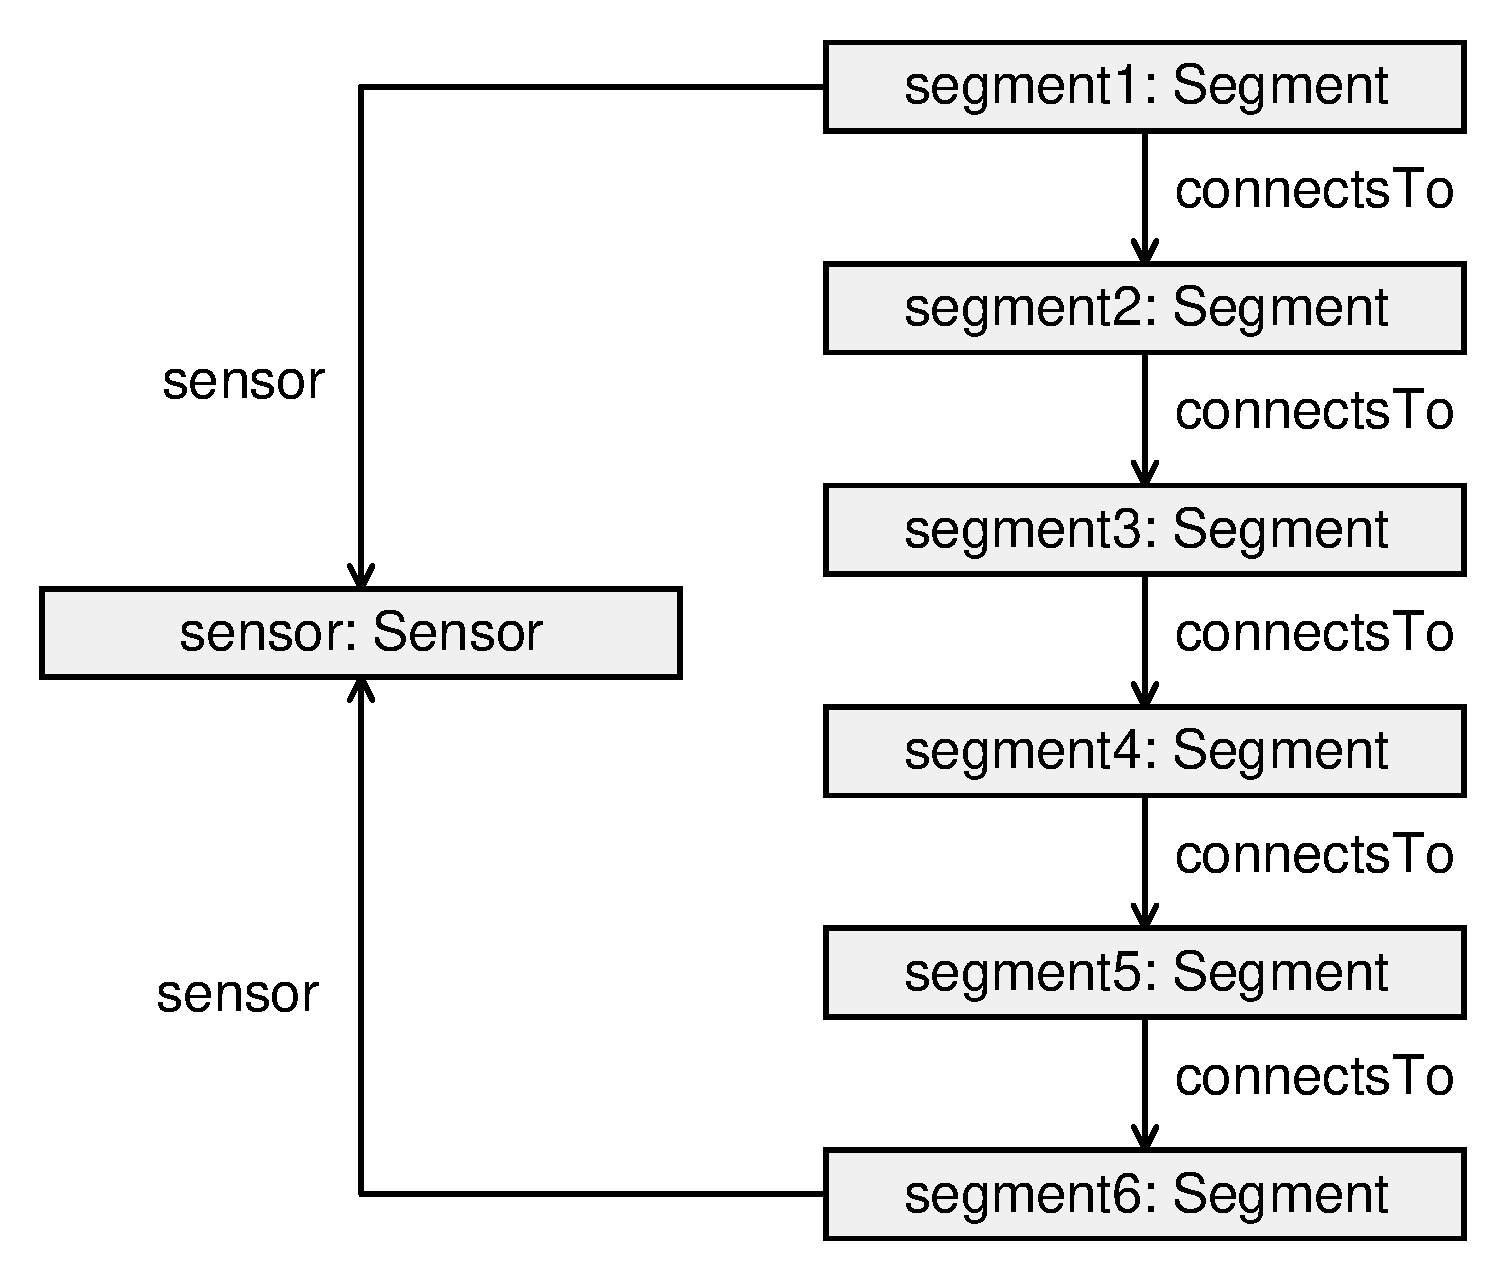
\includegraphics[scale=0.4]{figures/pattern-connectedsegments}
		\caption{The \textsf{ConnectedSegments} pattern.}
		\label{fig:pattern-connectedsegments}
\end{figure}

\paragraph{Relational algebraic form.} The \textsf{ConnectedSegments} query can be formalized in relational algebra as:

\begin{align*}
& \pi_{\mathit{id}} \sigma_{\mathit{Sensor}_1.\mathit{id} = \mathit{Sensor}_2.\mathit{id}} \big( \mathit{Sensor}_1 \\
& \quad \naturaljoin_{\mathit{Sensor}_1.\mathit{id} = \mathit{connectsTo}_1.\mathit{TrackElement}_1} \mathit{connectsTo}_1 \\
& \quad \naturaljoin_{\mathit{connectsTo}_1.\mathit{TrackElement_2} = \mathit{connectsTo}_2.\mathit{TrackElement}_1} \mathit{connectsTo}_2 \\
& \quad \naturaljoin_{\mathit{connectsTo}_2.\mathit{TrackElement_2} = \mathit{connectsTo}_3.\mathit{TrackElement}_1} \mathit{connectsTo}_3 \\
& \quad \naturaljoin_{\mathit{connectsTo}_3.\mathit{TrackElement_2} = \mathit{connectsTo}_4.\mathit{TrackElement}_1} \mathit{connectsTo}_4 \\
& \quad \naturaljoin_{\mathit{connectsTo}_4.\mathit{TrackElement_2} = \mathit{connectsTo}_5.\mathit{TrackElement}_1} \mathit{connectsTo}_5 \\
& \quad \naturaljoin_{\mathit{connectsTo}_5.\mathit{TrackElement_2} = \mathit{Sensor}_2.\mathit{id}} \mathit{Sensor}_2 \\
& \quad \\
& \big)
\end{align*}

%%%%%%%%%%%%%%%%%%%%%%%%%%%%%%%%%%%%%%%%%%%%%%%%%%%%%%%%%%%%%%%%%%%%%%%%%%%%%%%

\subsubsection{PosLength}

\paragraph{Description.} The \textsf{PosLength} well-formedness constraint requires that a segment must have positive length. Therefore, the query (\figref{fig:pattern-poslength}) checks for segments with a length less than or equal to zero. The SPARQL representation of the query is shown in \lstref{lst:poslength-sparql}.

\paragraph{Goal.} The query checks whether an object has an attribute. If it does, the value is checked. Checking attributes is a real world use case, even if a very simple one. Note that simple string checking is also measured in the Berlin SPARQL Benchmark~\cite{BSBM} and it concludes that for most tools the string comparison algorithm dominates the query time.

\begin{figure}[htb]
\centering
\begin{minipage}{0.9\textwidth}
  { \alignListing
    \sourceSPARQL{figures/queries/PosLength.sparql}}
  \caption{\textsf{PosLength} query in SPARQL.}
  \label{lst:poslength-sparql}
\end{minipage}
\end{figure}

\begin{figure}[htb]
		\centering
		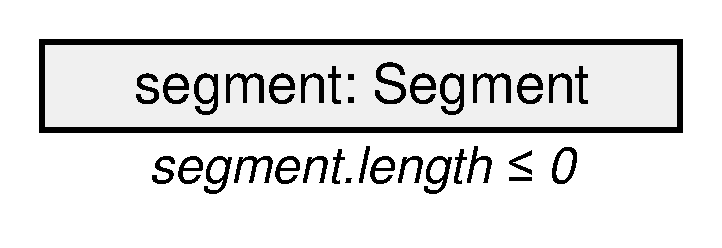
\includegraphics[scale=0.4]{figures/pattern-poslength}
		\caption{The \textsf{PosLength} pattern.}
		\label{fig:pattern-poslength}
\end{figure}

\paragraph{Relational algebraic form.} The \textsf{PosLength} query can be formalized in relational algebra as:

\[
\pi_{\mathit{id}} \left( \sigma_{\mathit{length} \leq 0} \left( \mathit{Sensor} \right) \right)
\]

%%%%%%%%%%%%%%%%%%%%%%%%%%%%%%%%%%%%%%%%%%%%%%%%%%%%%%%%%%%%%%%%%%%%%%%%%%%%%%%
\subsubsection{RouteSensor}

\paragraph{Description.} The \textsf{RouteSensor} well-formedness constraint requires that all sensors that are associated with a switch that belongs to a route must also be associated directly with the same route. Therefore, the query (\figref{fig:pattern-routesensor}) looks for sensors that are connected to a switch, but the sensor and the switch are not connected to the same route. The SPARQL representation of the query is shown in \lstref{lst:routesensor-sparql-nac}.

\paragraph{Goal.} This pattern checks for the absence of circles, so the efficiency of the join and the antijoin operations is tested.

\begin{figure}[htb]
\centering
\begin{minipage}{0.9\textwidth}
  { \alignListing
    \sourceSPARQL{figures/queries/RouteSensor_neg.sparql}}
  \caption{The \textsf{RouteSensor} query in SPARQL 1.1.}
  \label{lst:routesensor-sparql-nac}
\end{minipage}
\end{figure}

\paragraph{Remark.} Note that the negative application condition (NAC) part (\texttt{FILTER NOT EXISTS}) is a SPARQL 1.1 feature. In SPARQL 1.0, we have to use the approach shown in \lstref{lst:routesensor-sparql-nac10}.

\begin{figure}[htb]
\centering
\begin{minipage}{0.9\textwidth}
  { \alignListing
    \sourceSPARQL{figures/queries/RouteSensor.sparql}}
  \caption{The NAC of the \textsf{RouteSensor} pattern in SPARQL 1.0.}
  \label{lst:routesensor-sparql-nac10}
\end{minipage}
\end{figure}

\begin{figure}[htb]
		\centering
		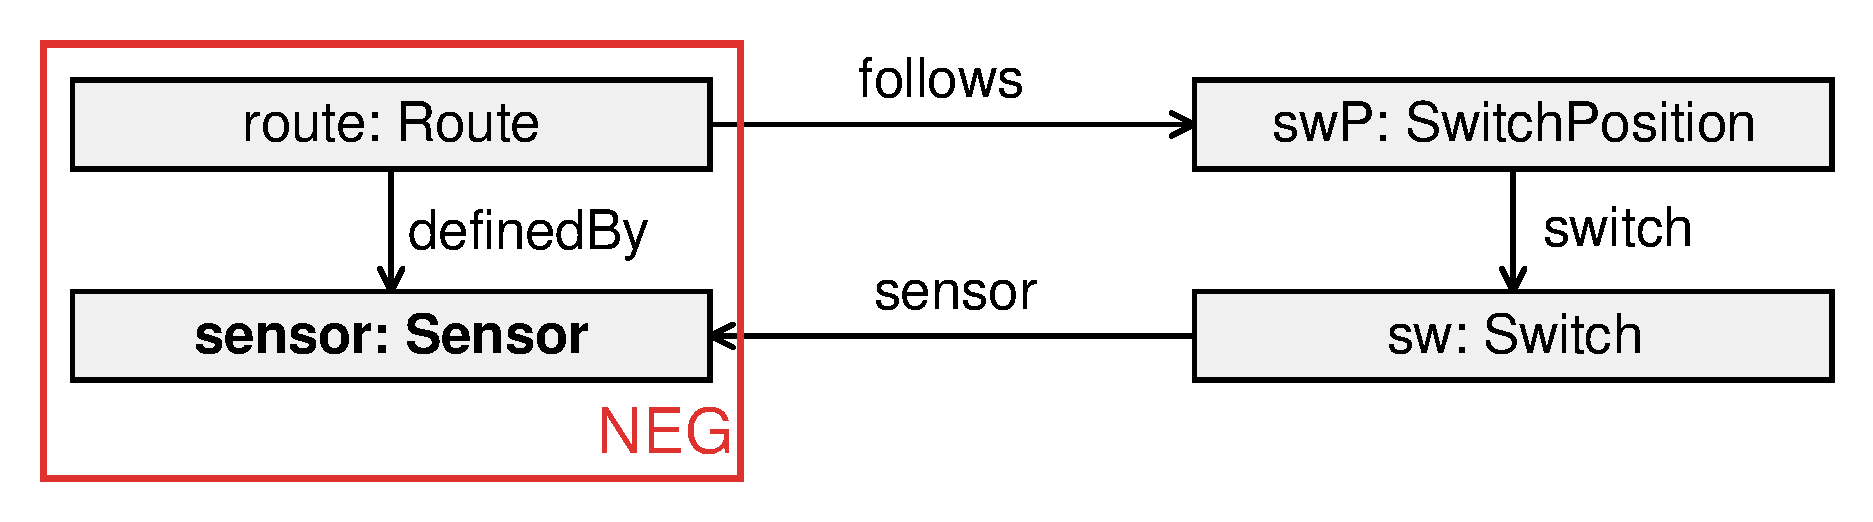
\includegraphics[scale=0.4]{figures/pattern-routesensor}
		\caption{The \textsf{RouteSensor} pattern.}
		\label{fig:pattern-routesensor}
\end{figure}

\paragraph{Relational algebraic form.}  The \textsf{RouteSensor} query can be formalized in relational algebra as:

\[
\pi_{\mathit{Route}} \big( \mathit{follows} \naturaljoin \mathit{switch} \naturaljoin \mathit{sensor} \antijoin \mathit{definedBy} \big)
\]

%%%%%%%%%%%%%%%%%%%%%%%%%%%%%%%%%%%%%%%%%%%%%%%%%%%%%%%%%%%%%%%%%%%%%%%%%%%%%%%
\subsubsection{SemaphoreNeighbor}

\paragraph{Description.} The \textsf{SemaphoreNeighbor} well-formedness constraint requires that the routes that are connected through sensors and track elements have to belong to the same semaphore. Therefore, the query (\figref{fig:pattern-semaphoreneighbor}) checks for routes which have an exit semaphore and a sensor connected to another sensor (which is in a definition of another route) by two track elements, but there is no other route that connects the same semaphore and the other sensor. The SPARQL representation of the query is shown in \lstref{lst:semaphoreneighbor-sparql}.

\paragraph{Goal.} This pattern checks for the absence of circles, so the efficiency of the join operation is tested. One-way navigable references are also present in the constraint, so the efficient evaluation of these are also tested. Subsumption inference is required, as the two track elements can be switches or segments.

\begin{figure}[htb]
\centering
\begin{minipage}{0.9\textwidth}
  { \alignListing
    \sourceSPARQL{figures/queries/SemaphoreNeighbor.sparql}}
  \caption{The \textsf{SemaphoreNeighbor} query in SPARQL.}
  \label{lst:semaphoreneighbor-sparql}
\end{minipage}
\end{figure}

\begin{figure}[htb]
		\centering
		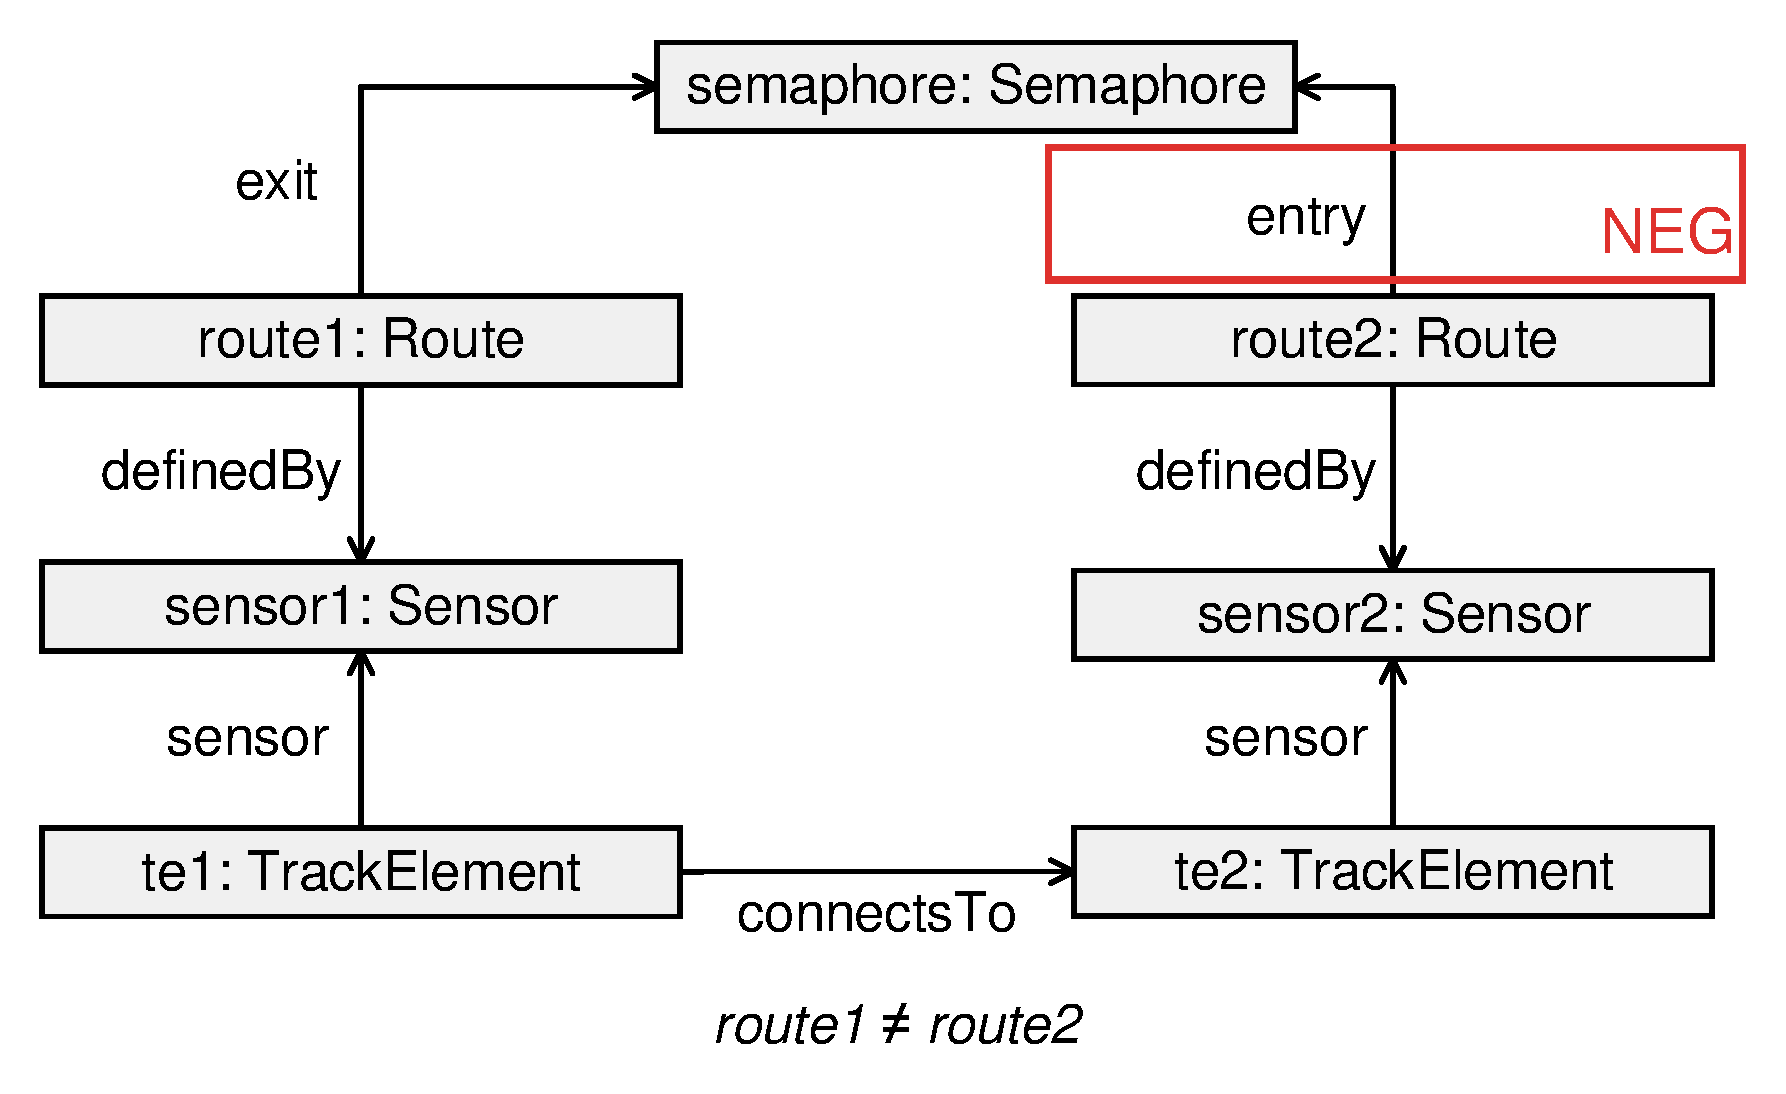
\includegraphics[scale=0.4]{figures/pattern-semaphoreneighbor}
		\caption{The \textsf{SemaphoreNeighbor} pattern.}
		\label{fig:pattern-semaphoreneighbor}
\end{figure}

\paragraph{Relational algebraic form.} The \textsf{SemaphoreNeighbor} query can be formalized in relational algebra as:

\begin{align*}
& \pi_{\mathit{entry.Route}} \big( \sigma_{\mathit{entry.Route} \neq \mathit{definedBy_2.Route}} \big( \\
& \quad \mathit{entry} \naturaljoin \mathit{definedBy_1} \naturaljoin \mathit{sensor_1} \naturaljoin \\
& \quad \mathit{connectsTo} \naturaljoin \mathit{sensor_2} \naturaljoin \mathit{definedBy_2} \antijoin \\
& \quad \left( \mathit{exit} \naturaljoin \mathit{definedBy_3} \right) \\
& \big) \big)
\end{align*}

%%%%%%%%%%%%%%%%%%%%%%%%%%%%%%%%%%%%%%%%%%%%%%%%%%%%%%%%%%%%%%%%%%%%%%%%%%%%%%%
\subsubsection{SwitchSensor}

\paragraph{Description.} The \textsf{SwitchSensor} well-formedness constraint requires that every switch must have at least one sensor connected to it. Therefore, the query (\figref{fig:pattern-switchsensor}) checks for switches that have no sensors associated with them. The SPARQL representation of the query is shown in \lstref{lst:switchsensor-sparql}.

\paragraph{Goal.} This query checks whether an object is connected to a relation. This pattern is common in more complex queries, \eg it is used in the \textsf{RouteSensor} and the \textsf{SemaphoreNeighbor} queries.

\begin{figure}[htb]
\centering
\begin{minipage}{0.9\textwidth}
  { \alignListing
    \sourceSPARQL{figures/queries/SwitchSensor_neg.sparql}}
  \caption{The \textsf{SwitchSensor} query in SPARQL.}
  \label{lst:switchsensor-sparql}
\end{minipage}
\end{figure}


\begin{figure}[htb]
	\centering
	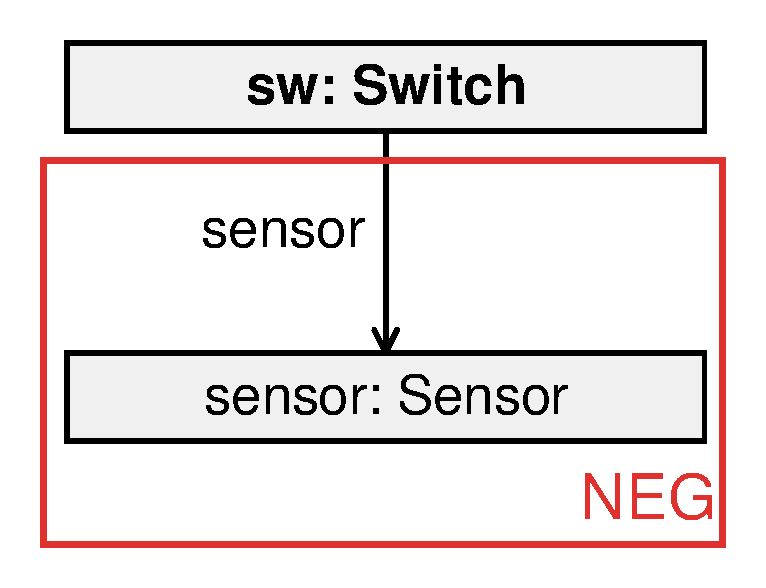
\includegraphics[scale=0.4]{figures/pattern-switchsensor}
	\caption{The \textsf{SwitchSensor} pattern.}
	\label{fig:pattern-switchsensor}
\end{figure}

\paragraph{Relational algebraic form.} The \textsf{SwitchSensor} query can be formalized in relational algebra as:

$$ \mathit{Switch} \antijoin \mathit{Sensor} $$

%%%%%%%%%%%%%%%%%%%%%%%%%%%%%%%%%%%%%%%%%%%%%%%%%%%%%%%%%%%%%%%%%%%%%%%%%%%%%%%
\subsubsection{SwitchSet}

\paragraph{Description.}The entry semaphore of a route may only show GO if all switches along the route are in the position prescribed by the route. The SPARQL representation of the query is shown in \lstref{lst:switchset-sparql}.

\paragraph{Goal.} This pattern tests the efficiency of the join and filtering operations.

\begin{figure}[htb]
\centering
\begin{minipage}{0.9\textwidth}
  { \alignListing
    \sourceSPARQL{figures/queries/SwitchSet.sparql}}
  \caption{The \textsf{SwitchSet} query in SPARQL.}
  \label{lst:switchset-sparql}
\end{minipage}
\end{figure}


\begin{figure}[htb]
	\centering
	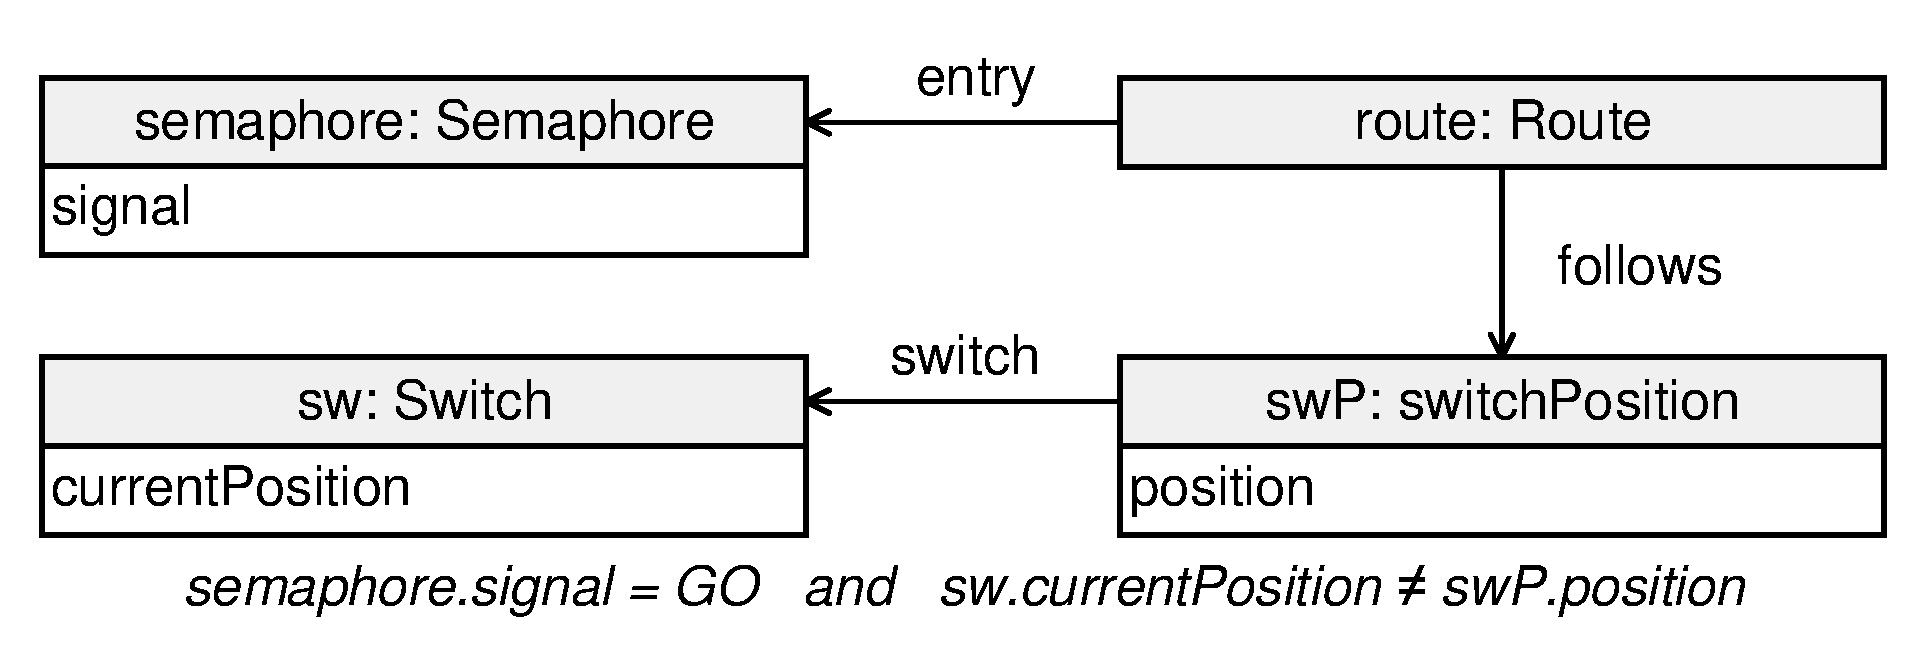
\includegraphics[scale=0.4]{figures/pattern-switchset}
	\caption{The \textsf{SwitchSet} pattern.}
	\label{fig:pattern-switchset}
\end{figure}

\paragraph{Relational algebraic form.} The \textsf{SwitchSet} query can be formalized in relational algebra as:

\begin{align*}
& \pi_{\mathit{id}} \sigma_{\mathit{Semaphore}.\mathit{signal} = \mathrm{"GO"} \wedge \mathit{Switch}.\mathit{currentPosition} \neq \mathit{SwitchPosition}.\mathit{position}} \big( \mathit{Route} \\
& \quad \naturaljoin_{\mathit{Route}.\mathit{entry} = \mathit{Semaphore}.\mathit{id}} \mathit{Semaphore} \\
& \quad \naturaljoin_{\mathit{Route}.\mathit{id} = \mathit{follows}.\mathit{Route}} \mathit{follows} \\
& \quad \naturaljoin_{\mathit{follows}.\mathit{SwitchPosition} = \mathit{SwitchPosition}.\mathit{id}} \mathit{SwitchPosition} \\
& \quad \naturaljoin_{\mathit{SwitchPosition}.\mathit{id} = \mathit{switch}.\mathit{SwitchPosition}} \mathit{switch} \\
& \quad \naturaljoin_{\mathit{switch}.\mathit{Switch} = \mathit{Switch}.\mathit{id}} \mathit{Switch} \\
& \big)
\end{align*}

\subsection{Transformations}
\label{sec:transformatios}

In the \emph{edit} phase the model is modified to change the result set returned in the succeeding re-check phase.

The Train Benchmark defines model transformations for each query. The transformations are also represented as graph transformations. The insertions are shown in green with a \guillemotleft{}new\guillemotright{} caption, while deletions are marked with a red cross and a \guillemotleft{}del\guillemotright{} caption. In general, the goal of these transformations is to remove a subset of the invalid elements from the model.

\begin{table}[htb]
	\centering
	\scriptsize
	\begin{tabular}{r|r|r|r|r|r|r|r|r|r|}
	\cline{2-9}
	& \multicolumn{4}{ c| }{\bf Inject (modify = 10)} & \multicolumn{4}{ c| }{\bf Repair (modify = Res1 × 10\%)} \\ \hline
	\multicolumn{1}{ |r| }{\bf\#Objects} & \bf \#Sensors & \bf Result1 & \bf Modify RS & \bf Result2 & \bf \#Sensors & \bf Result1 & \bf Modify RS & \bf Result2 \\ \hline
	\multicolumn{1}{ |r| }{6032}         & 928 & 19 & 10 & 29 & 967 & 94 & 9 & 85 \\ \hline
	\multicolumn{1}{ |r| }{11710}        & 1804 & 41 & 10 & 51 & 1936 & 193 & 19 & 174 \\ \hline
	\multicolumn{1}{ |r| }{23180}        & 3575 & 68 & 10 & 76 & 3545 & 348 & 34 & 314 \\ \hline
	\multicolumn{1}{ |r| }{46728}        & 7210 & 140 & 10 & 150 & 6691 & 642 & 64 & 578 \\ \hline
	\multicolumn{1}{ |r| }{87396}        & 13465 & 264 & 10 & 274 & 13650 & 1301 & 130 & 1171 \\ \hline
	\multicolumn{1}{ |r| }{175754}       & 27074 & 510 & 10 & 520 & 27190 & 2606 & 260 & 2346 \\ \hline
	\multicolumn{1}{ |r| }{354762}       & 54653 & 1048 & 10 & 1058 & 55708 & 5324 & 532 & 4792 \\ \hline
	\multicolumn{1}{ |r| }{708770}       & 109185 & 2071 & 10 & 2081 & 110291 & 10623 & 1062 & 9561 \\ \hline
	\multicolumn{1}{ |r| }{1415954}      & 218140 & 4215 & 10 & 4224 & 219305 & 21097 & 2109 & 18988 \\ \hline
	\multicolumn{1}{ |r| }{2837336}      & 437089 & 8501 & 10 & 8510 & 437025 & 41762 & 4176 & 37586 \\ \hline
	\end{tabular}
	\caption{Modification in the \textsf{RouteSensor} test case.}
	\label{tbl:modify_RouteSensor}
\end{table}

\autoref{tbl:modify_RouteSensor}. shows the instance model characteristics and the effect of the modify phase in the \textsf{RouteSensor} case. The first column counts the number of instance model elements. The second and the fifth column show the number of Sensors in the model. The two scenarios process different instance models and modify them differently:

\begin{itemize}
	\item In the \emph{Inject scenario} (where a developer is assumed to sit in front of an editor) the initial number of constraint violating elements are low (0.3\% of model elements for the \textsf{RouteSensor} case), so it can be understood and resolved by a user using the editor.
	
	During the modification the user always performs 10 random edits (fixed low constant) which \emph{increase} the number of erroneous elements. These edit operations modify only some elements of the model and do not add or remove modules containing multiple instance model elements.

	\item In the \emph{Repair scenario} the initial number of errors is higher (1.5\% of objects for the \textsf{RouteSensor} case). This scenario models the case when these errors are (partially) processed by a model transformation program automatically.

	In the edit phase the program modifies 10\% of the elements of the result set retrieved from the batch query. These modifications always correct an invalid element in the model, so the number of invalid elements \emph{decreases} (see \autoref{tbl:modify_type}).

\end{itemize}


\autoref{tbl:modify_type}. displays the effect of model changes to the result set size and the type of edit operations (add, update, delete).

\begin{table}[h]
	\centering
	\begin{tabular}{l|l|l|l|l|l|}
	\cline{2-5}
	& \multicolumn{2}{ c| }{\bf Inject} & \multicolumn{2}{ c| }{\bf Repair} \\ \cline{2-5}
	& \bf Modification type & \bf RSS change & \bf Modification type & \bf RSS change \\ \hline
	\multicolumn{1}{ |l| }{\bf ConnectedSegments} & Insert and delete & Increase & Insert and delete & Decrease \\ \hline
	\multicolumn{1}{ |l| }{\bf PosLength}         & Update            & Increase & Update            & Decrease \\ \hline
	\multicolumn{1}{ |l| }{\bf RouteSensor}       & Delete            & Increase & Delete            & Decrease \\ \hline
	\multicolumn{1}{ |l| }{\bf SemaphoreNeighbor} & Update            & Increase & Update            & Decrease \\ \hline
	\multicolumn{1}{ |l| }{\bf SwitchSensor}      & Delete            & Increase & Add               & Decrease \\ \hline
	\multicolumn{1}{ |l| }{\bf SwitchSet}         & Update            & Increate & Update            & Decrease \\ \hline
	\end{tabular}
	\caption{Modification type for the queries.}
	\label{tbl:modify_type}
\end{table}

\begin{figure}
        \centering
        \begin{subfigure}[b]{0.7\textwidth}
                \centering
                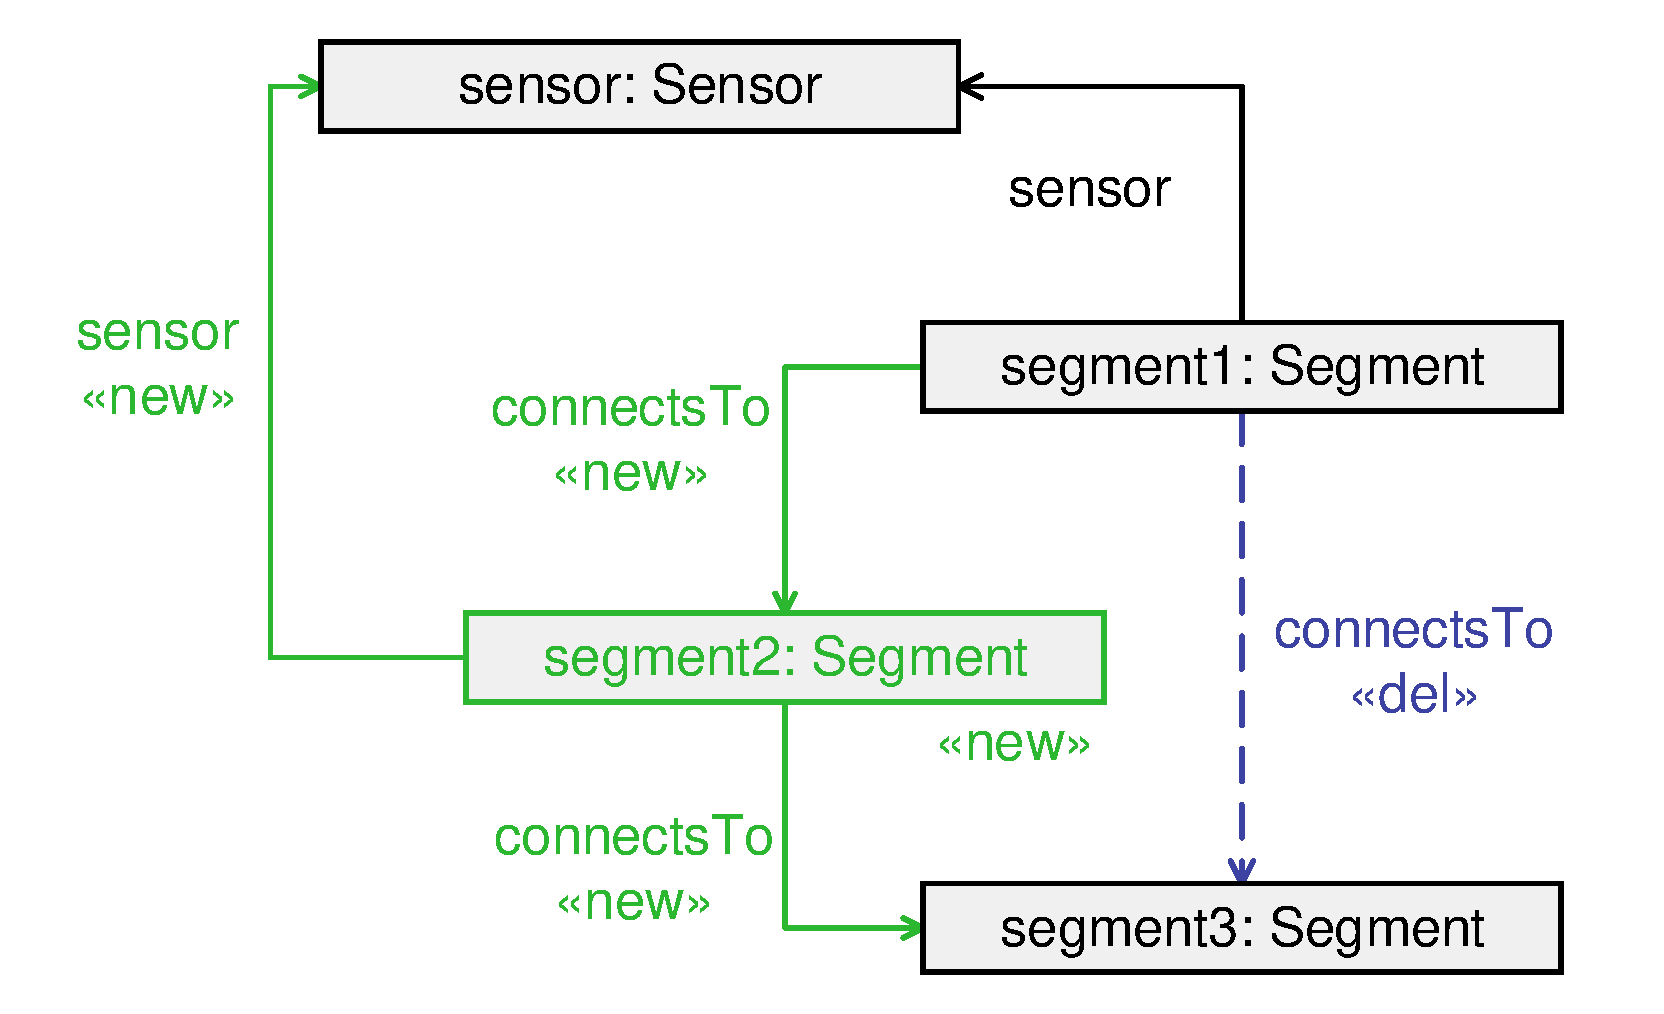
\includegraphics[scale=0.4]{figures/transformation-inject-connectedsegments}
                \caption{\textsf{ConnectedSegments}}
                \label{fig:transformation-inject-connectedsegments}
        \end{subfigure}
        ~
        \begin{subfigure}[b]{0.4\textwidth}
        		\centering
                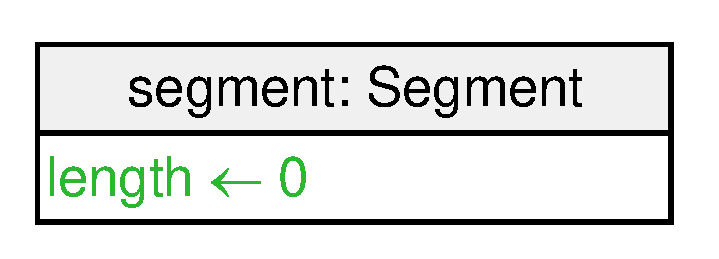
\includegraphics[scale=0.4]{figures/transformation-inject-poslength}
                \caption{\textsf{PosLength}}
                \label{fig:transformation-inject-poslength}
        \end{subfigure}%
        ~
        \begin{subfigure}[b]{0.6\textwidth}
                \centering
                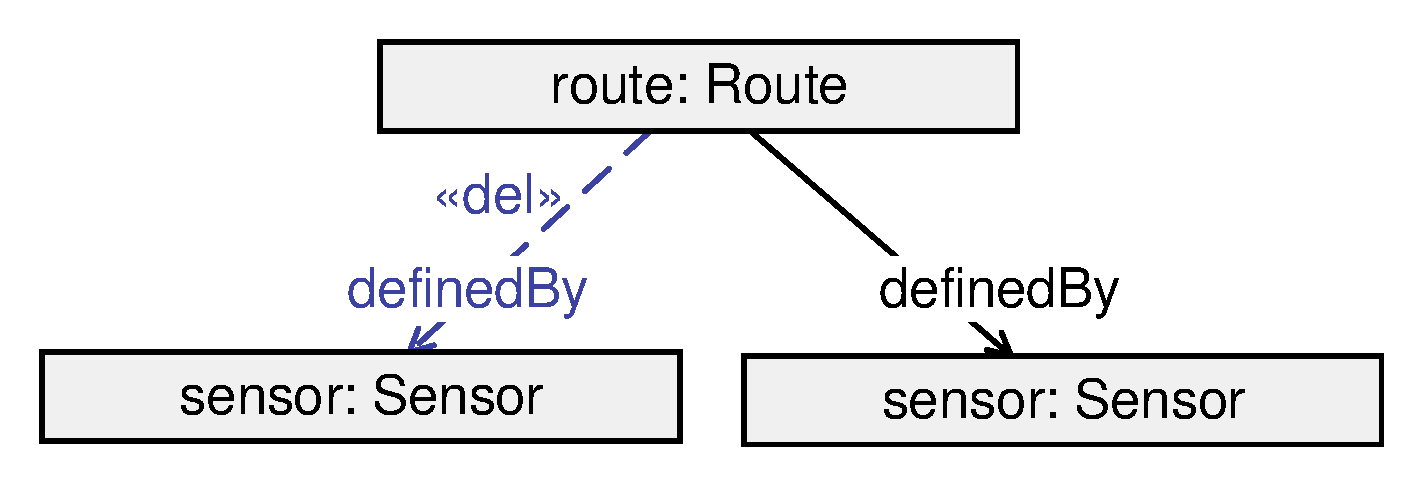
\includegraphics[scale=0.4]{figures/transformation-inject-routesensor}
                \caption{\textsf{RouteSensor}}
                \label{fig:transformation-inject-routesensor}
        \end{subfigure}
        ~
        \begin{subfigure}[b]{0.4\textwidth}
                \centering
                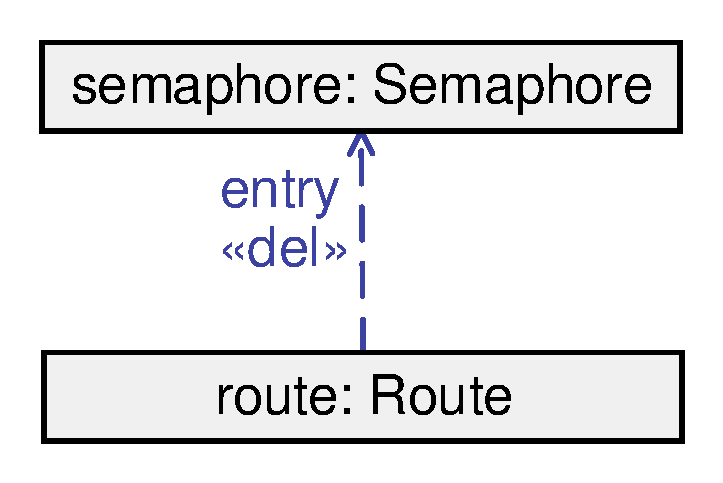
\includegraphics[scale=0.4]{figures/transformation-inject-semaphoreneighbor}
                \caption{\textsf{SemaphoreNeighbor}}
                \label{fig:transformation-inject-semaphoreneighbor}
        \end{subfigure}%
        ~
        \begin{subfigure}[b]{0.6\textwidth}
                \centering
                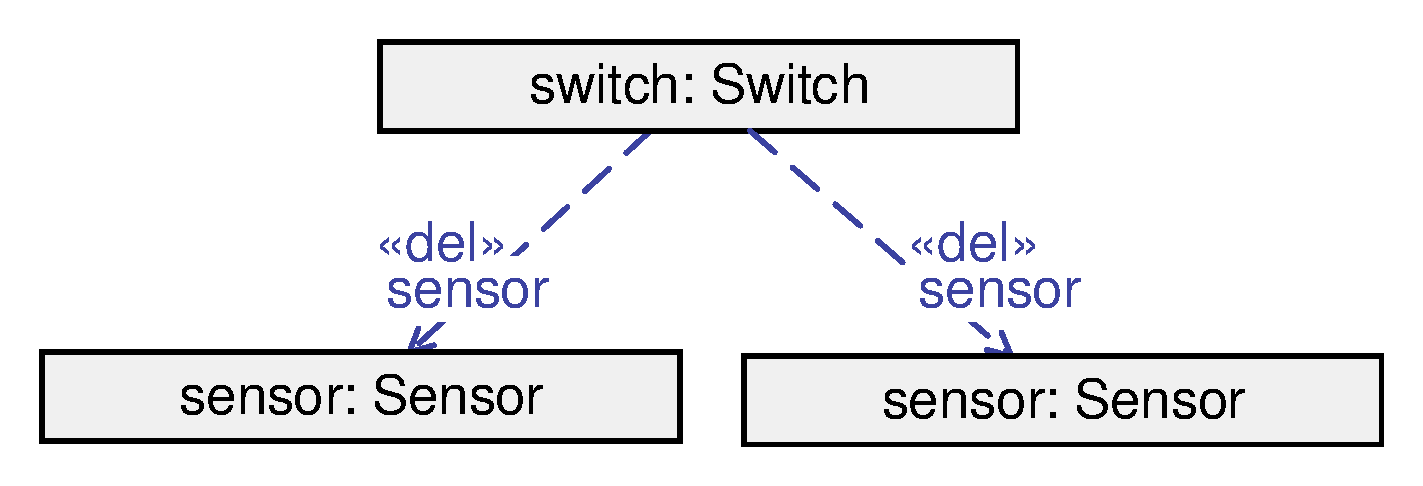
\includegraphics[scale=0.4]{figures/transformation-inject-switchsensor}
                \caption{\textsf{SwitchSensor}}
                \label{fig:transformation-inject-switchsensor}
        \end{subfigure}
        ~
        \begin{subfigure}[b]{0.6\textwidth}
                \centering
                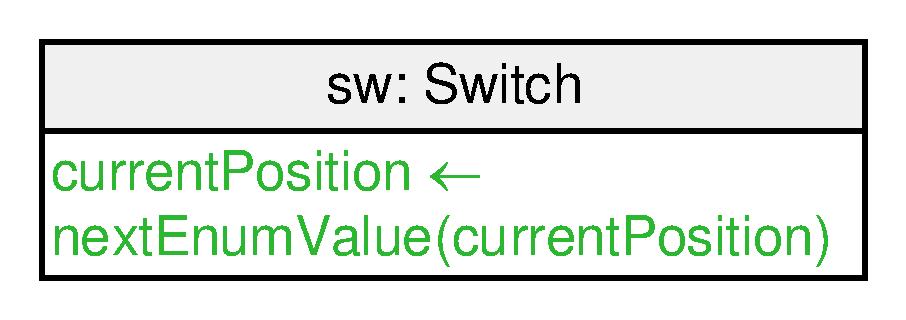
\includegraphics[scale=0.4]{figures/transformation-inject-switchset}
                \caption{\textsf{SwitchSet}}
                \label{fig:transformation-inject-switchset}
        \end{subfigure}
        \caption{Transformations in the \textsf{Inject} scenario.}
        \label{fig:transformations-repair}
\end{figure}


The modifications in more detail:
\begin{itemize}
  \item \emph{Inject scenario:} in this case elements to be edited are selected from the whole instance model, \ie they may be valid or invalid. 
  \begin{itemize}
    
    \item \emph{PosLength:} Randomly selected \emph{segments'} \emph{length} attribute is updated to 0, which means that an error is injected (\figref{fig:transformation-inject-poslength}).\footnote{In EMF this means that an \texttt{int} attribute is set (updated), while in other representations (\eg RDF databases) first the assertion about the old value is removed and the assertion stating the new value of the length is inserted.}
    
    \item \emph{RouteSensor:} The \emph{definedBy} edges between the randomly selected \emph{routes} and their \emph{first} connected \emph{sensor} are removed (at most one edge for each route, see~\figref{fig:transformation-inject-routesensor}).
    
    \item \emph{SemaphoreNeighbor:} Errors are introduced by disconnecting the \emph{entry} edge of the selected \emph{routes} (\figref{fig:transformation-inject-semaphoreneighbor}). (According to the metamodel, a \emph{route} may only have 0 or 1 \emph{entry} edges).

    \item \emph{SwitchSensor:} Errors are injected by randomly selecting \emph{switches} and deleting all their edges to \emph{sensors}. If the chosen \emph{switch} was invalid, it did not have such an edge, so no edges are deleted and the \emph{switch} stays invalid. If the chosen \emph{switch} was valid, it will become invalid (\figref{fig:transformation-inject-switchsensor}).
        
\end{itemize}
  
  
\begin{figure}
        \centering
        \begin{subfigure}[b]{\textwidth}
        		\centering
                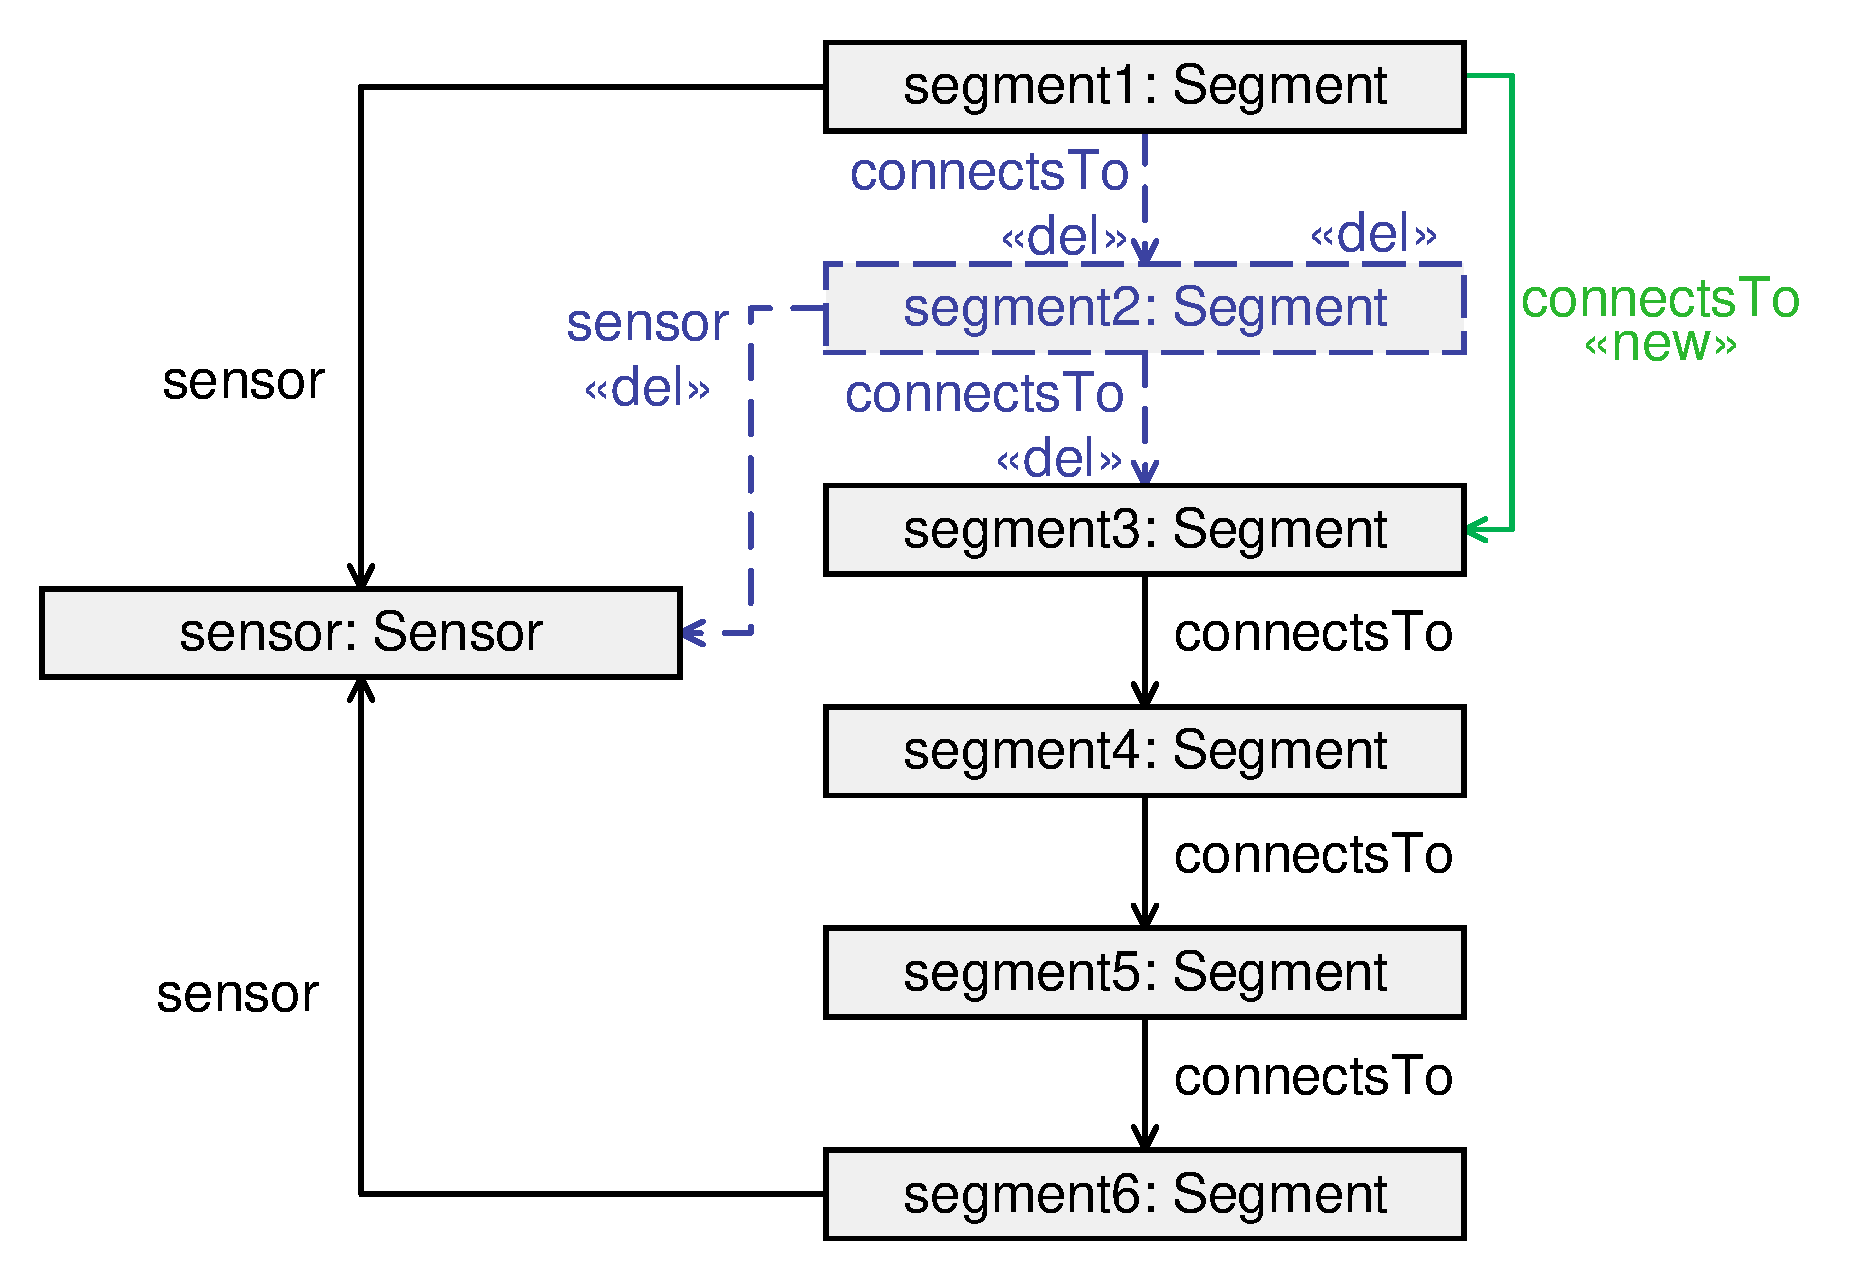
\includegraphics[scale=0.2]{figures/transformation-repair-connectedsegments}
                \caption{\textsf{ConnectedSegments}}
                \label{fig:transformation-repair-connectedsegments}
        \end{subfigure}
        ~
        \begin{subfigure}[b]{\textwidth}
        		\centering
                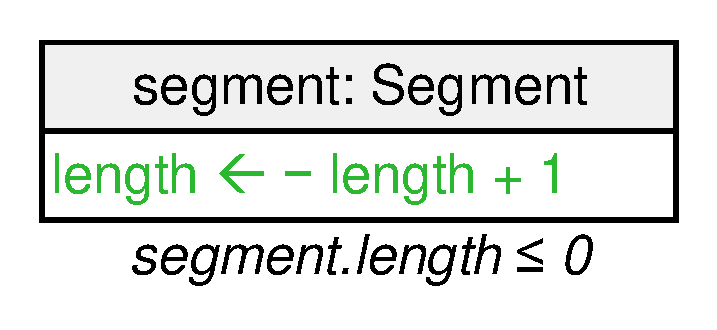
\includegraphics[scale=0.2]{figures/transformation-repair-poslength}
                \caption{\textsf{PosLength}}
                \label{fig:transformation-repair-poslength}
        \end{subfigure}
        ~
        \begin{subfigure}[b]{\textwidth}
                \centering
                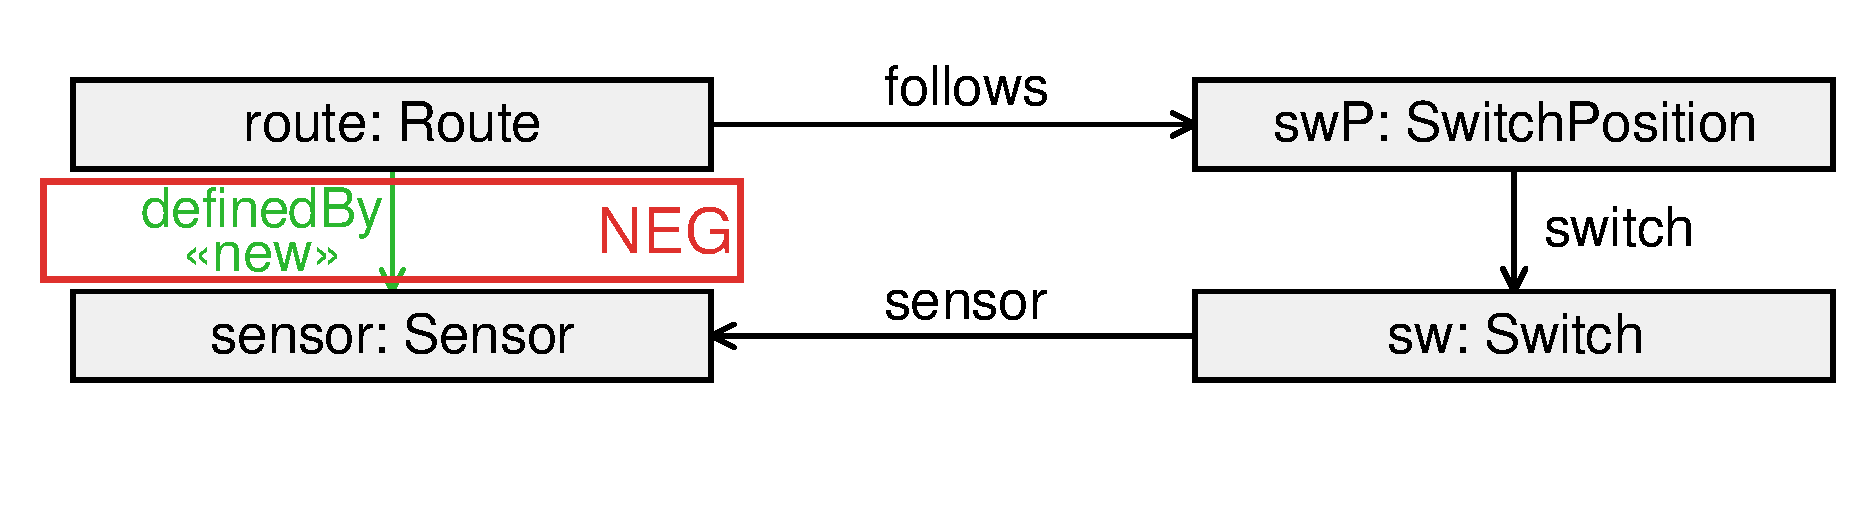
\includegraphics[scale=0.2]{figures/transformation-repair-routesensor}
                \caption{\textsf{RouteSensor}}
                \label{fig:transformation-repair-routesensor}
        \end{subfigure}
        ~
        \begin{subfigure}[b]{\textwidth}
                \centering
                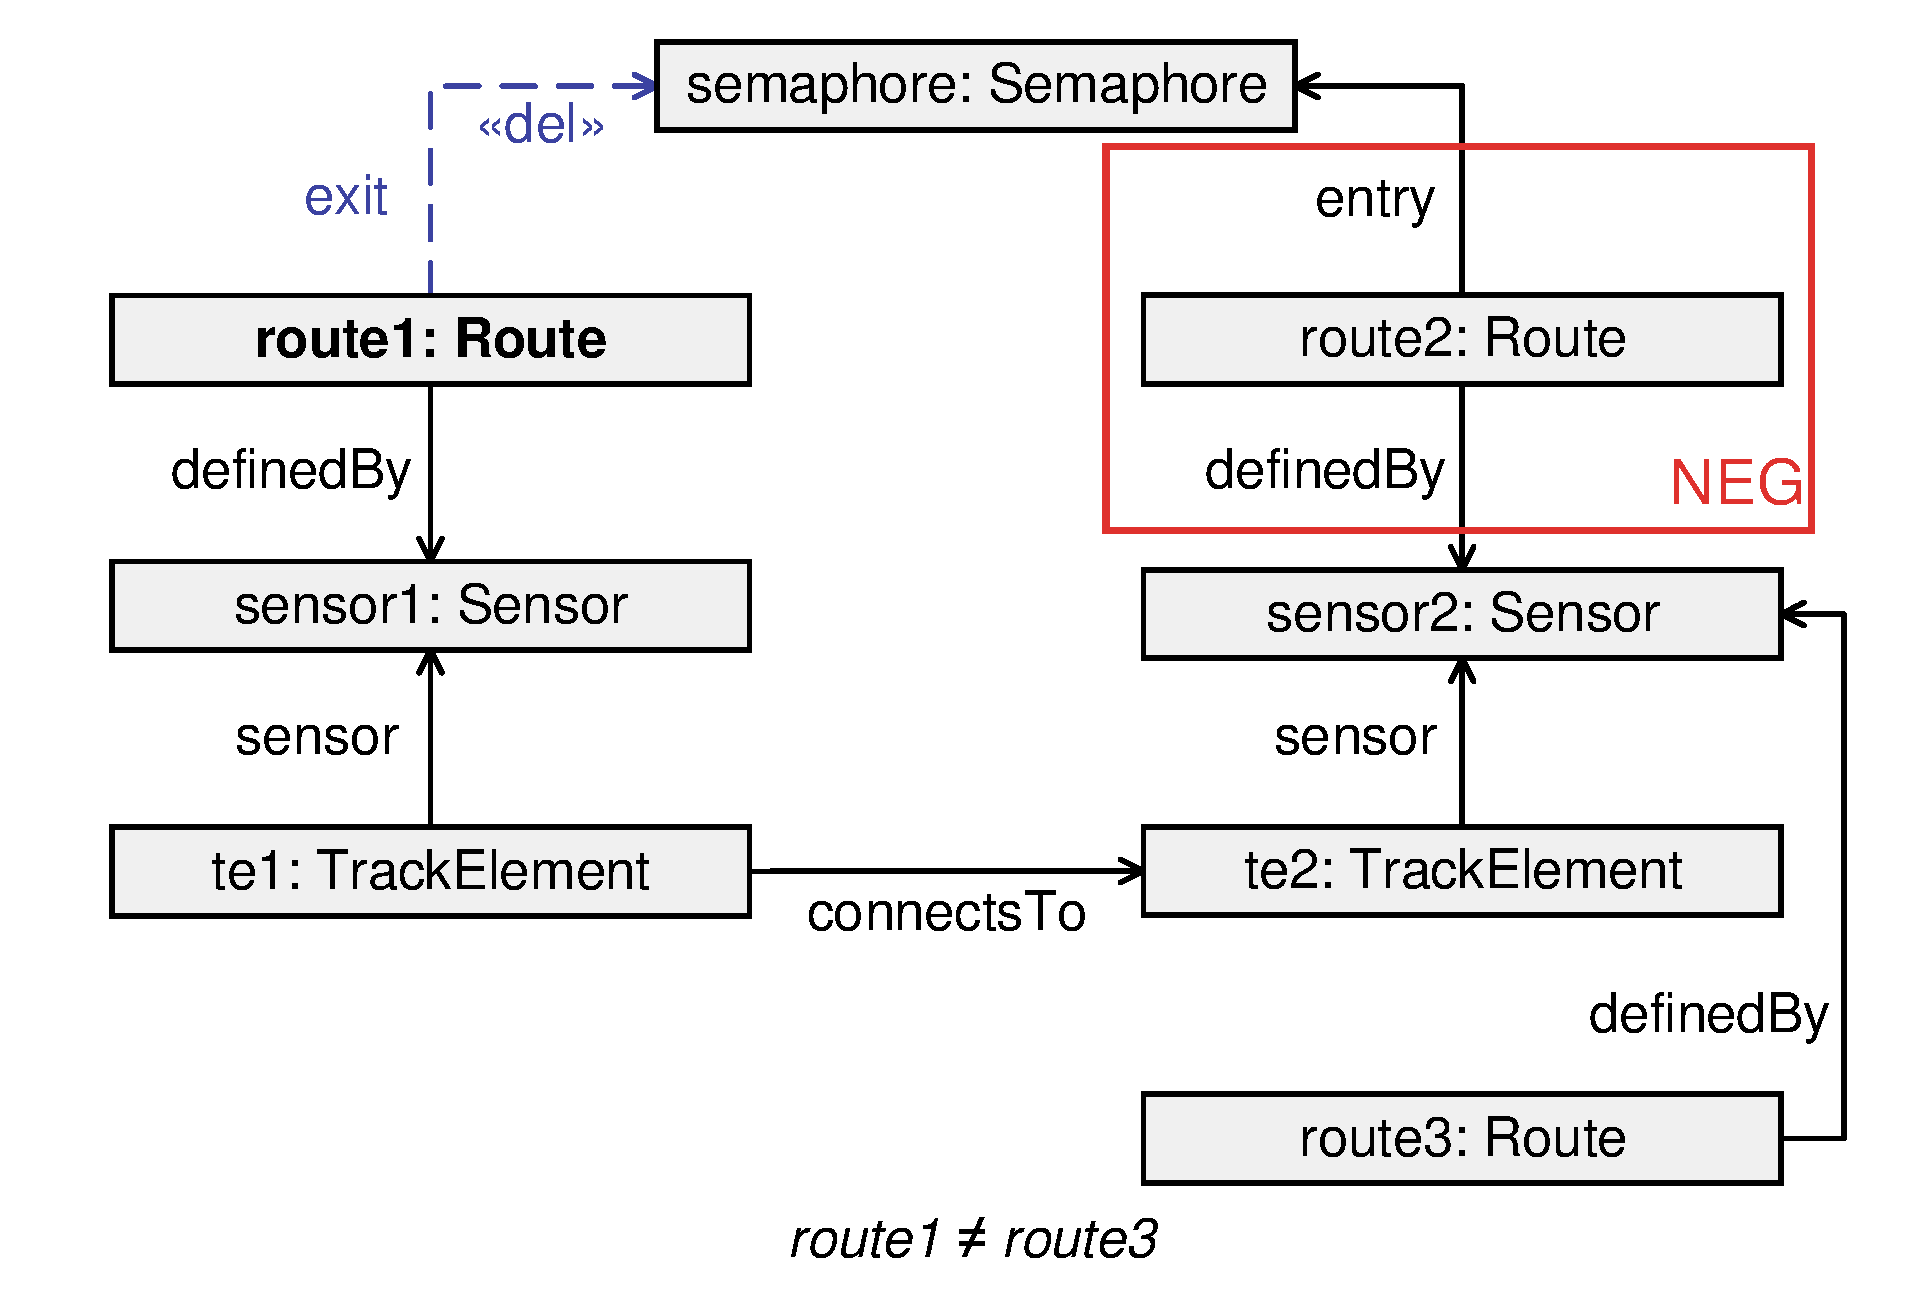
\includegraphics[scale=0.2]{figures/transformation-repair-semaphoreneighbor}
                \caption{\textsf{SemaphoreNeighbor}}
                \label{fig:transformation-repair-semaphoreneighbor}
        \end{subfigure}
        ~
        \begin{subfigure}[b]{\textwidth}
                \centering
                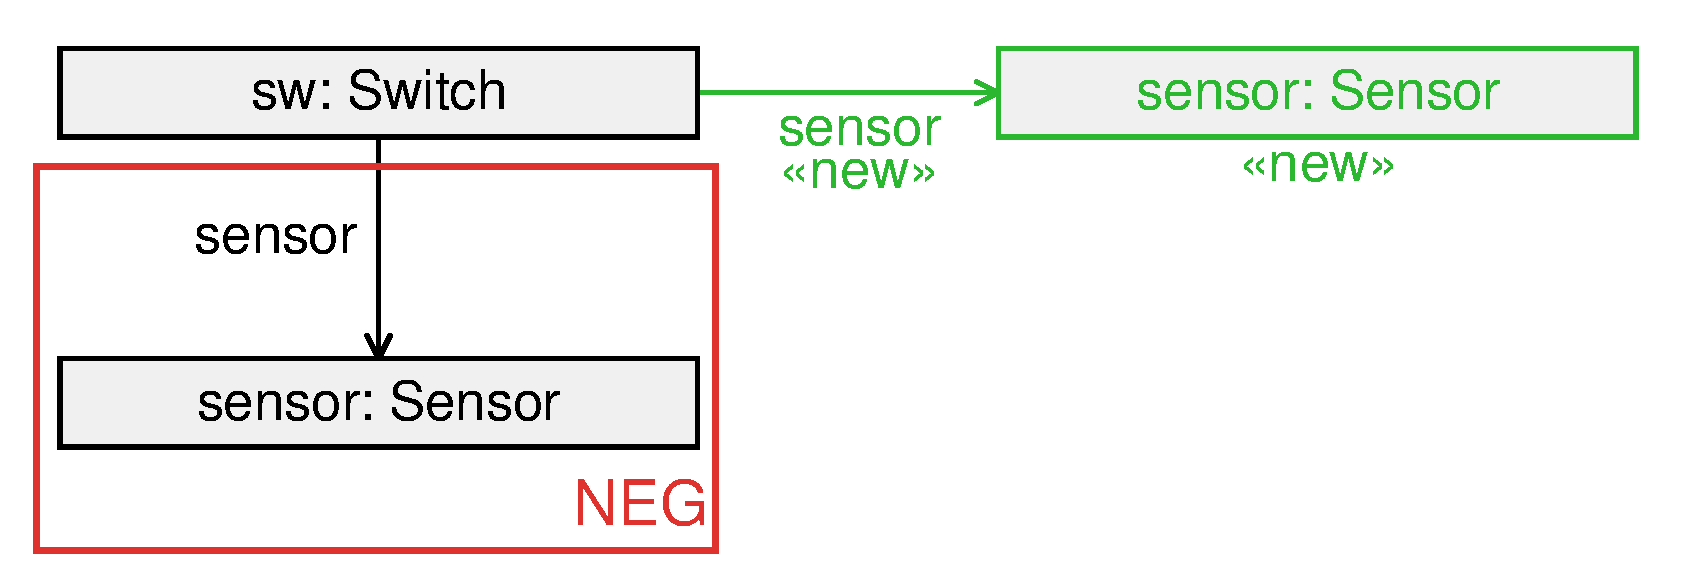
\includegraphics[scale=0.2]{figures/transformation-repair-switchsensor}
                \caption{\textsf{SwitchSensor}}
                \label{fig:transformation-repair-switchsensor}
        \end{subfigure}        
        ~
        \begin{subfigure}[b]{\textwidth}
                \centering
                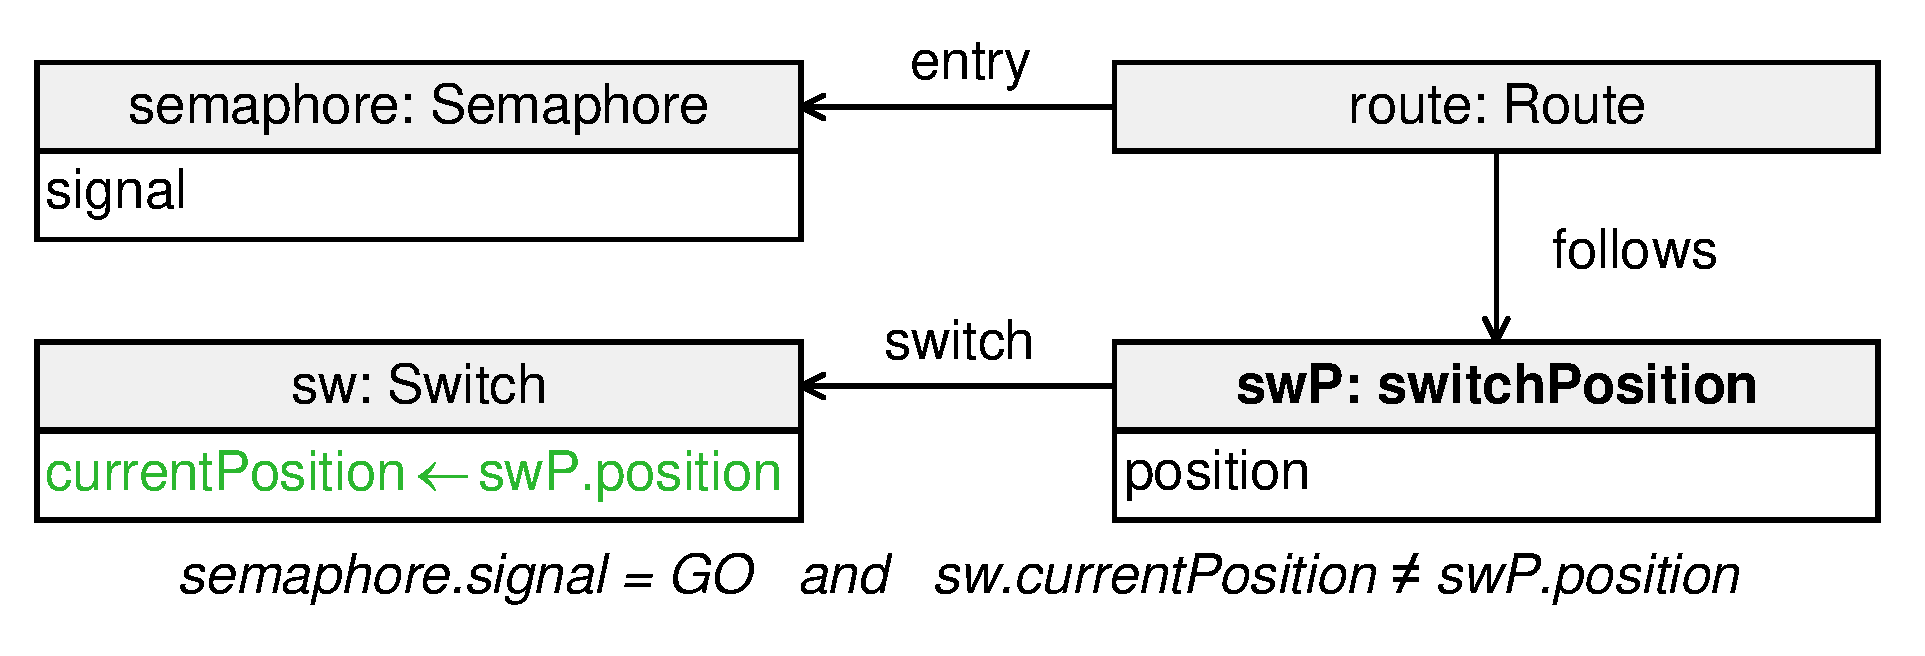
\includegraphics[scale=0.2]{figures/transformation-repair-switchset}
                \caption{\textsf{SwitchSet}}
                \label{fig:transformation-repair-switchset}
        \end{subfigure}
        \caption{Transformations in the \textsf{Repair} scenario.}
        \label{fig:transformations-repair}
\end{figure}
  
  \item \emph{Repair scenario:} in this case elements to be edited are selected from the result of the previous query. The transformations provide quick fix-like repair operations.
  \begin{itemize}
    
    \item \emph{PosLength:} Random elements are selected from the set of invalid \emph{segments} and their values are updated to $- \mathit{oldValue} + 1$ (\figref{fig:transformation-repair-poslength}).
    
    \item \emph{RouteSensor:} Randomly selected invalid \emph{sensors} are disconnected from the \emph{switch}, which means that the constraint will no longer apply (\figref{fig:transformation-repair-routesensor}).
    
    \item  \emph{SemaphoreNeighbor:} Disconnect \emph{exit} references of randomly selected invalid \emph{routes}, resulting in a structure where the constraint must not hold for the actual route (\figref{fig:transformation-repair-semaphoreneighbor}).
        
    \item \emph{SwitchSensor:} Random elements are selected from the set of invalid \emph{switches} and are connected to newly created \emph{sensors}.
    
    In EMF this means the creation of a new Sensor which is added to the switch and also to the root container object. In ontology the triples asserting the connection between the new Sensor and the Switch, as well as its type are inserted into the knowledge base (\figref{fig:transformation-repair-switchsensor}).
    
  \end{itemize}
\end{itemize}


\subsection{Instance Model Generation}
\label{sec:instanceGeneration}

In the first phase of the benchmark, a previously generated \concept{instance model} is loaded from the file system. These models are systematically generated based on the metamodel and on the model queries. Randomized instance model fragments are generated and connected to each other. The generation process takes care of controlling the number of matches for all model queries.

To break symmetry, the exact number of elements and cardinalities are randomized. This brings artificially generated models \emph{closer to real world instances}, and \emph{prevents query tools from this kind of efficient storing} of instance models. During the generation of the railway system model, errors are injected at random positions. The initial number of constraint violating elements that are low (below one percent of the total number of elements), and are deterministically placed, thanks to \emph{pseudorandom} generation. These errors have to be found in the check phase of the benchmark, and can be corrected during the edit phase.

\begin{figure}[htb]
\begin{center}
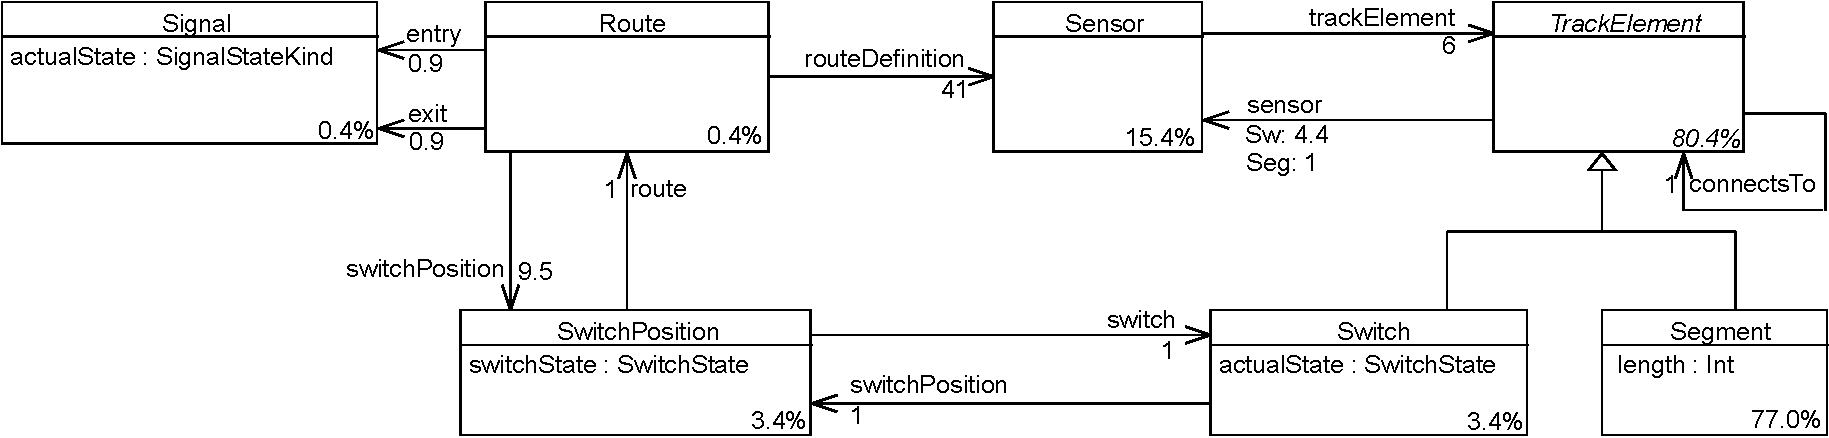
\includegraphics[width=\textwidth]{figures/instance/TrainMMb.pdf}
\caption{The railway metamodel and instance model characteristics.}
\label{fig:metamodel-instance-characteristics}
\end{center}
\end{figure}

To show some characteristics of the generated instance models, the distribution of the object types and the average number of edges for each object are presented in \autoref{fig:metamodel}. In the case of classes the percentage of instances is shown: \eg 3.4\% of the model elements are instance of the class \emph{Switch}, 77.0\% are \emph{Segment}s, thus 80.4\% are \emph{TrackElement}s. The average number of the given relation for an instance is displayed for associations: \eg there are 9.5 \emph{switchPosition} relations in average for every instance of the \emph{Route} class.

\section{Extended version}
\label{specification-extended}

Section \ref{specification-original} describes a benchmark that can be used to compare performance of different tools. This Sections extends this benchmarking conecpt by characterizing instance models and queries by metrics, and evaluate which tools are the most sensitive to which metrics. 

\subsection{Overview}
\label{sec:benchmark_overview}
The aim of our metrics and benchmarking scenarios is to give a precise mechanism for identifying key factors in selecting between different query evaluation technologies.

The presented metrics for our evaluation (see in~\autoref{sec:benchmark-metrics}) were constructed based on a set of already and widely used metrics, extended with two more specific ones that aims to give a gross upper bound on the cost of query evaluation.

For the benchmark scenario we opted for a simple execution schema that represents a batch validation scenario. This is the same as the first two phase of the original benchmark. See \figref{fig:phases} and \autoref{sec:phases} for a description of the \emph{read} and \emph{check} phases. 


\subsection{Metrics}
\label{sec:benchmark-metrics}

Our investigation relies on a selection of metrics that quantitatively describe
the task of a certain query, independently of the actual strategy or technological solution
that provides the query results. Broadly speaking, such a querying task consist
of (a) an instance model, (b) a query specification that defines what results
should be yielded, (c) a runtime context in which the queries are evaluated,
such as the frequency of individual query evaluations and model manipulation
inbetween.

The metrics discussed in the following, characterize instance models, queries or their combination, without characterizing a unique property of a specific graph/query description language or environment. Most of these metrics have previously been defined by other sources, while others are newly proposed in this paper.

\subsubsection{Metrics for Instance Model Only}
Clearly, properties of the instance model may have a direct effect on query
performance, e.g.\ querying larger models may consume  more resources.

% do NOT press Esc+Q !!! (or re-wrap comment!)
A first model metric is model size, which can be defined either as the
number of objects (metric \code{countNodes}), the number of references (edges)
between objects (\code{countEdges}), the number of attribute value assignments
(not used in the paper);
%\code{countValueAssignments} 
or some combination of
these three, such as their sum (\code{countTriples}), which is basically the
total number of model elements / RDF triples. This is complemented by the number
of different classes the objects in the model belong to (\code{countTypes}), and
the instance count distribution of the classes. %( TODO todo \todo{todo}).
Additional important model metrics characterize the distribution of the
out-degrees and in-degrees (the number of edges incident on an object),
particularly the maximum and average degrees (\code{maxInDegree},
\code{maxOutDegree}, \code{avgInDegree} and \code{avgOutDegree}).
 
The metrics discussed above have been defined e.g.\ in~\cite{COLD2012-analysis-DBLP:conf/semweb/StarkaSM12}, along with other
metrics such as the relative frequencies of the edge label sequences of directed
paths of length 2 or 3.
 
\subsubsection{Metrics for Query Specification Only}
The query specification is a decisive factor of performance as well, as complex
queries may be costly to evaluate. Such query metrics can be defined separately,
in several query formalisms. Due to the
close analogies between graph patterns and SPARQL queries, we can consider these
metrics applying to graph pattern-like queries in general. This allows us to
formulate and calculate metrics expressed on the graph patterns interpreted by
\incquery{}, and characterize the complexity of the equivalent SPARQL query with
the same metric value.

As superficial metrics for graph pattern complexity, we propose the number of
variables (\code{numVariables}) and the number of parameter variables
(\code{numParameters}); the number of pattern edge constraints
(\code{numEdgeConstraints}) and the number of attribute check constraints
(\code{numAttrChecks}); finally the maximum depth of nesting NACs
(\code{nestedNacDepth}). Some of these are similar/equivalent to 
SPARQL query metrics defined in~\cite{SPLODGE}. Other metrics proposed
by~\cite{SPLODGE} are mostly aimed at measuring special properties relevant to
certain implementation strategies.

\subsubsection{Metrics for Combination of Query and Instance Model}
The following two metrics (defined previously in literature) characterize the
query and the instance model together.

The most trivial such metric is the cardinality of the query results (metric
\code{countMatches}); intuitively, a query with a larger result set typically
takes longer to evaluate on the same model, while a single query is typically
more expensive to evaluate on models where it has more matches. The metric
\code{selectivity} is proposed by~\cite{SPLODGE}, is the ratio of the
number of results to the number of model elements (i.e.\ 
$countMatches/countTriples$).


\subsubsection{New Metrics for Assessing Query Evaluation Difficulty}
We propose two more metrics that take query and instance model characteristics into account. 
Our aim is to provide a gross upper bound on
the cost of query evaluation. We consider all \emph{enumerable} constraints in
the query, for which it is possible to enumerate all tuples of variables
satisfying it; thus edge constraints and pattern composition are enumerable,
while NACs and attribute checks in general are not. At any given state of
evaluation, a hypothetical search-based query engine has either already
identified a single occurrence of an enumerable constraint $c$ (e.g.\ a single
instance of an edge type for the corresponding edge constraint), or not; there
are therefore $\abs{c}+1$ possible cases for $c$, where $\abs{c}$ is the number
of different ways that $c$ can be satisfied in the model. This gives
$\prod_{c}{1+\abs{c}}$ as the overestimate of the search space of the query
evaluator. To make this astronomical figure manageable, we propose the absolute
difficulty metric (\code{absDifficulty}) as the logarithm of the search space
size, i.e.\ $ln\prod_{c}{(1+\abs{c})} = \sum_{c}{ln(1+\abs{c})}$.
 
The result size is a lower bound of query evaluation cost, since query
evaluation takes at least as much time or memory as the number of results. It is
therefore expected that queries with a high number of matches also score high on
the absolute difficulty metric. To compensate for this, the relative difficulty
metric (\code{relDifficulty}) is defined as
$ln\frac{\prod_{c}{(1+\abs{c})}}{1+countMatches} = \sum_{c}{ln(1+\abs{c})} -
ln(1+countMatches)$, expressing the logarithm of the ``challenge'' the query
poses -- this is how much worse a query engine can do than the lower bound. 
If the relative metric is a low figure, than the cost of query evaluation will not
be much worse than the optimum, regardless of the query evaluation strategy. It
can be easily shown that if a part of a graph pattern is extracted as a helper
pattern that is used via pattern composition, then the sum of the relative
difficulties of the two resulting patterns will be the same as the relative
difficulty of the original pattern. This suggests that this metric should be
treated as additive over dependent queries, and also that it is worth extracting
common parts of multiple patterns into reusable helper patterns.

\subsection{Modified Metamodel}

\begin{figure}[Hhtb]
\begin{center}
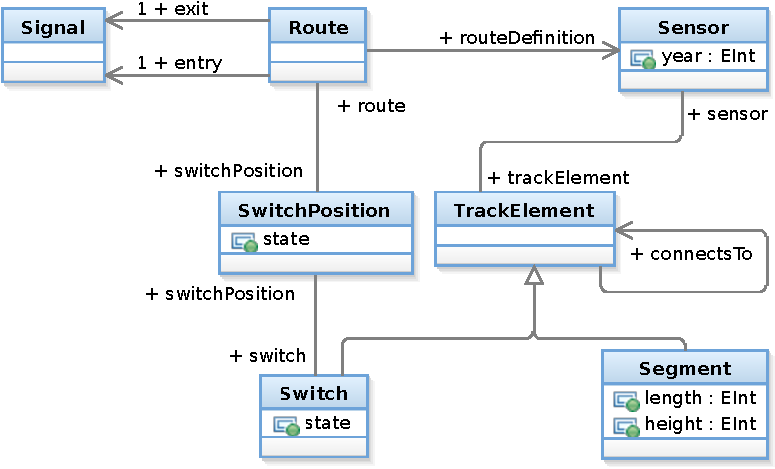
\includegraphics[width=12cm]{figures/TrainMMMet.pdf}
\caption{The railway metamodel (metrics version).}
\label{fig:metamodel-met}
\end{center}
\end{figure}

The metamodel used for merics evaluation is depicted in \figref{fig:metamodel-met}. This is similar to the one presented in \autoref{sec:domain}, but cardinality constraints are mostly omitted, and \emph{height} and \emph{year} integer attributes are introduced for classes Segment and Sensor respectively. This gives higher freedom for the instance model generator, and more queries can be defined for attribute checks.

\subsection{Instance Models for the Modified Metamodel}
\label{sec:benchmark-models}

Models are characterized by their size and structure. Here size refers to the cardinalities of node and edge types. The fact that increasing model size tends to increase the cost of queries is intuitively self evident (and also empirically confirmed e.g.\ by our previous experiments~\cite{icgt08-bhrv,models10}). Handling large models in real life is a great chellenge, but model structure (that determines which nodes are connected to each other by which edges) must also be taken into account, which here means edge distribution of nodes. Different edge distributions also present in real-world networks: the internet or protein-protein interaction networks show \emph{scale-free} characteristics~\cite{barabasi_network_2004}, while in other areas self-healing algorithms for \emph{binomial computer networks} are studied~\cite{binomial-self-healing}. Average degree can impact performance greatly, which is a typical property of different model kinds. For example, software models have usually nodes with \emph{low degree}, while social models are usually \emph{dense graphs}. 

We have conducted the experiments on synthetic models, generated automatically
with our model builder, belonging to three \concept{model families}  (without
comparing them directly to real world ones, leaving it as a future work). All
generated models within a family have the same approximate size; though there is
some random variation due to the generation process (see later), with low
standard deviation (e.g.\ measured as 0.3\% in family $A$).  Family $A$ models are relatively dense graphs
(\texttildelow 26 edges/nodes, i.e.\ metric \code{avgOutDegree}) with 1.8 million
total model elements (metric \code{numTriples}); family $B$ models are equally
dense, but are scaled back to only 113 thousand elements; finally family $C$
models have almost 1.3 million model elements that form a relatively sparse
graph ($8.4-8.7$ edges/nodes).

Each model of a family has the same (expected) number of instances for any given
type. However, these models of the same size still differ in their internal
\concept{structure}. Given the cardinalities of each type, our generator first
created the instance sets of node types, along with generating attribute values
according to an associated distribution. Then for each edge type, the generator
created edge instances (with the given expected cardinality) between instances
of the source type and instances of the target type. The structure of the graph
is induced by the method of choosing which source node and which target node to
connect. We have applied the following four methods, each taking as input the
set $S$ of source node candidates, the set $T$ of target node candidates, and
the expected cardinality $e$ of the edge type. %\begin{description}

  \emph{Binomial case.} Inspired by the well-known Erdős-Rényi model of random
  graphs~\cite{erdos1960erg}, the first approach is to take each pair of source and
  target nodes, and draw an edge between them with a given probability $p$. This makes the
  expected cardinality of edges $e = p \times \abs{S} \times \abs{T}$, thus $p$
  is chosen as $\frac{e}{\abs{S} \times \abs{T}}$. The degrees of nodes will be
  binomially distributed, e.g.\ out-degrees with parameters $\abs{T}$ and $p$.
  
  \emph{Hypergeometric case.} While the previous solution ended up with a
  random number of edges (with expected value $e$), this slightly different
  approach will generate exactly $e$ edges, by taking each pair of source and
  target nodes, and randomly selecting $e$ from them into the graph. The degrees
  will be hypergeometrically distributed, e.g.\ out-degrees with parameters
  $\abs{S} \times \abs{T}$, $\abs{T}$ and $e$.
    
  \emph{Regular case.} In software engineering models, one often finds for a
  given edge type that out-degrees of all nodes of the source type are roughly
  equal, and the same is true for in-degrees. This motivated a method that tries
  to uniformly (but randomly) divide $e$ edges between the source nodes, so that
  the difference between any two out-degrees is at most 1; while also dividing
  the same edges between the target nodes, with a similar restriction on
  in-degrees.
  
  \emph{Scale-free case.} It has been observed in many different disciplines
  that degree distributions of certain large graphs follow a power law,
  especially growing / evolving graphs with the \emph{preferential attachment}
  property (a new edge is more likely to connect to a node which already has a
  higher degree). We have used a variant of the preferential attachment
  bipartite graph generator algorithm of~\cite{RandomNetworkGeneration2005} to
  generate the connections from source nodes to target nodes.
 
The four generation methods induced significantly different degree
distributions. 
This and other differences are shown in \autoref{tbl:instance_metric_values}.
 
One-to-many relationships were treated in a special way to meet the multiplicity
restriction. In particular, a single top-level container element (not depicted
in the metamodel figure, neither involved in any queries) was used to contain
all elements; it therefore has an outgoing containment edge for every other
object, thereby ``polluting'' the \code{maxOutDegree} metric.


\begin{table*}[tp]
	\centering
	\resizebox{\textwidth}{!}{
	\begin{tabular}{|c|l|r|r|r|r|r|r|r|r|}%{|l|c|c|c|c|c|c|c|c|c|c|}
	\hline 
	\textbf{Model Family} & \textbf{Model structure} & \textbf{countNodes} & \textbf{countEdges} & \textbf{countTriples} & \textbf{countTypes} & \textbf{avgOutDegree} & \textbf{avgInDegree} & \textbf{maxOutDegree} & \textbf{maxInDegree}\\ \hline
	A & Regular & 63289 & 1646386 & 1811752 & 7 & 26.01 & 26.01 & 63288 & 44\\ \hline
	A & Binomial & 63289 & 1649179 & 1814545 & 7 & 26.06 & 26.06 & 63288 & 69\\ \hline
	A & HyperGeo & 63289 & 1646386 & 1811752 & 7 & 26.01 & 26.01 & 63288 & 74\\ \hline
	A & Scalefree & 63289 & 1660033 & 1825399 & 7 & 26.23 & 26.23 & 63288 & 10390\\ \hline
	
	B & Regular & 3954 & 102839 & 113170 & 7 & 26.01 & 26.01 & 3953 & 44\\ \hline
	B & Binomial & 3954 & 102984 & 113315 & 7 & 26.05 & 26.05 & 3953 & 64\\ \hline
	B & HyperGeo & 3954 & 102839 & 113170 & 7 & 26.01 & 26.01 & 3953 & 69\\ \hline
	B & Scalefree & 3954 & 96029 & 106360 & 7 & 24.29 & 24.29 & 3953 & 918\\ \hline
	
	C & Regular & 120001 & 1040000 & 1280001 & 7 & 8.67 & 8.67 & 120000 & 13\\ \hline
	C & Binomial & 120001 & 1041323 & 1281324 & 7 & 8.68 & 8.68 & 120000 & 30\\ \hline
	C & HyperGeo & 120001 & 1040000 & 1280001 & 7 & 8.67 & 8.67 & 120000 & 29\\ \hline
	C & Scalefree & 120001 & 1012858 & 1252859 & 7 & 8.44 & 8.44 & 120000 & 8929\\ \hline
	
	\end{tabular} 
	}
	\caption{Values of model metrics on the generated instance models.}
	\label{tbl:instance_metric_values}
	\end{table*}


\subsection{Benchmark Queries}
\label{sec:benchmark-queries}

Based on the previously defined metrics for query specification and based on the
metamodel, six series of model query specifications were systematically
constructed. Each query series includes four to seven model queries that aim to
be different in only one of the defined model query metrics. Executing a query
series on the same model and tool results in a data series that shows how the
tool is scalable according to the represented model metric.

\subsubsection{\code{Locals} Query Series for the \code{numVariables} Metric}
Five queries were defined, where each one includes the same number of edge
constraints, but the number of local variables increases. 

It can be realized using the \code{Segment} type and \code{connectsTo}
reference, so it means that only one node type and reference type is used in
these patterns and the focus is on the structure of the patterns. The simple
graph based visualisation of these pattern structures is shown in \figref{fig:aselocals},
where the node drawn with empty circle represents the
single pattern parameter.

\tikzstyle{every node}=[circle, draw, fill=black, inner sep=0pt, minimum
							width=4pt, scale=0.5, node distance=2cm]
\begin{figure}[ht]
	\centering
	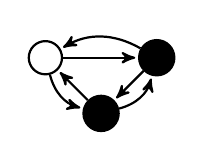
\begin{tikzpicture}[->,>=stealth',shorten >=1pt,auto, thick,main
	  node/.style={circle,fill=black,draw,font=\sffamily\Large\bfseries,inner
	  sep=0pt, minimum width=4pt}]
	
	  \node[main node] (3) [] {3};
	  \node[main node, fill=white, minimum width=12pt] (1) [above left of=3]{};
	  \node[main node] (2) [above right of=3] {2};
	
	  \path[every node/.style={font=\sffamily\small}]
	    (1) edge node {} (2)
	        edge [bend right] node {} (3)
	    (2) edge [bend right] node [right] {} (1)
	        edge node {} (3)
	    (3) edge node [right] {} (1)
	        edge [bend right] node {} (2);
	\end{tikzpicture}
	\hspace{3mm}
	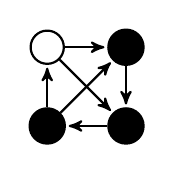
\begin{tikzpicture}[->,>=stealth',shorten >=1pt,auto,thick,main
	  node/.style={circle,fill=black,draw,font=\sffamily\Large\bfseries,inner
	  sep=0pt, minimum width=4pt}]
	
	  \node[main node, fill=white, minimum width=12pt] (1) []{};
	  \node[main node] (2) [right of=1] {2};
	  \node[main node] (3) [below of=1] {3};
	  \node[main node] (4) [right of=3] {4};
	
	  \path[every node/.style={font=\sffamily\small}]
	    (1) edge node {} (2)
	        edge node {} (4)
	    (2) edge node {} (4)
	    (3) edge node {} (1)
	        edge node {} (2)
	    (4) edge node {} (3)
	        ;
	\end{tikzpicture}
	\hspace{3mm}
	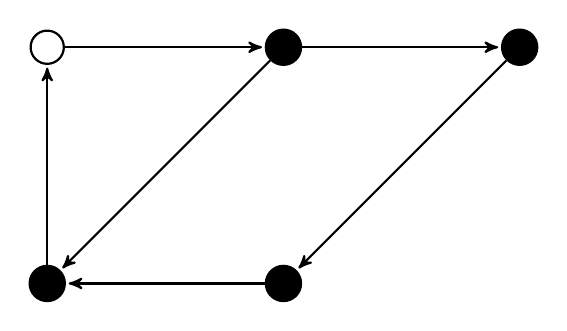
\begin{tikzpicture}[->,>=stealth',shorten >=1pt,auto,node distance=3cm,
	  thick,main
	  node/.style={circle,fill=black,draw,font=\sffamily\Large\bfseries,inner
	  sep=0pt, minimum width=4pt}]
	
	  \node[main node, fill=white, minimum width=12pt] (1) []{};
	  \node[main node] (2) [right of=1] {2};
	  \node[main node] (3) [right of=2] {3};
	  \node[main node] (4) [below of=1] {4};
	  \node[main node] (5) [right of=4] {5};
	
	  \path[every node/.style={font=\sffamily\small}]
	    (1) edge node {} (2)
	    (2) edge node {} (3)
	        edge node {} (4)
	    (3) edge node {} (5)
	    (4) edge node {} (1)
	    (5) edge node {} (4)
	        ;
	\end{tikzpicture}
	\hspace{3mm}
	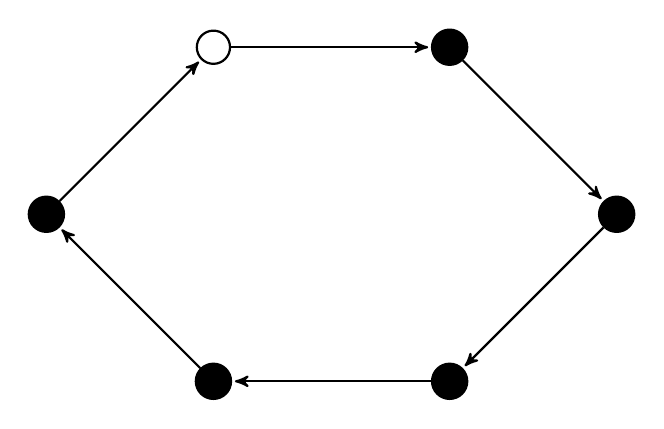
\begin{tikzpicture}[->,>=stealth',shorten >=1pt,auto,node distance=3cm,
	  thick,main
	  node/.style={circle,fill=black,draw,font=\sffamily\Large\bfseries,inner
	  sep=0pt, minimum width=4pt}]
	
	  \node[main node, fill=white, minimum width=12pt] (1) []{};
	  \node[main node] (2) [right of=1] {2};
	  \node[main node] (3) [below right of=2] {3};
	  \node[main node] (4) [below left of=3] {4};
	  \node[main node] (5) [left of=4] {5};
	  \node[main node] (6) [below left of=1] {6};
	
	  \path[every node/.style={font=\sffamily\small}]
	    (1) edge node {} (2)
	    (2) edge node {} (3)
	    (3) edge node {} (4)
	    (4) edge node {} (5)
	    (5) edge node {} (6)
	    (6) edge node {} (1)
	        ;
	\end{tikzpicture}
	\hspace{3mm}
	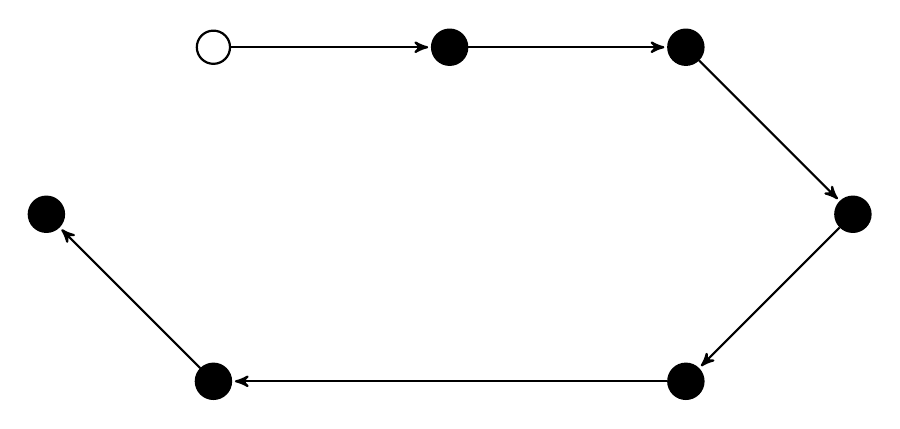
\begin{tikzpicture}[->,>=stealth',shorten >=1pt,auto,node distance=3cm,
	  thick,main
	  node/.style={circle,fill=black,draw,font=\sffamily\Large\bfseries,inner
	  sep=0pt, minimum width=4pt}]
	
	  \node[main node, fill=white, minimum width=12pt] (1) []{};
	  \node[main node] (2) [right of=1] {2};
	  \node[main node] (3) [right of=2] {3};
	  \node[main node] (4) [below right of=3] {4};
	  \node[main node] (5) [below left of=4] {5};
	  \node[main node] (7) [below left of=1] {7};
	  \node[main node] (6) [below right of=7] {6};
	
	  \path[every node/.style={font=\sffamily\small}]
	    (1) edge node {} (2)
	    (2) edge node {} (3)
	    (3) edge node {} (4)
	    (4) edge node {} (5)
	    (5) edge node {} (6)
	    (6) edge node {} (7)
	        ; 
	\end{tikzpicture}
	\caption{\codeCap{Locals} patterns}
	\label{fig:aselocals}
\end{figure}	

\subsubsection{\code{Refs} Query Series for the \code{numEdgeConstraints}
Metric}
%Like the query series for metric \code{numVariables}, 
The \code{Refs} query series is
also constructed based on the \code{Segment} type and \code{connectsTo}
reference. 

Here, the number of edge constraints increases along the series, but
the number of local variables is constant in all of the generated four queries.
The visualisation of these pattern structures is shown in \figref{fig:aserefs}. 

\begin{figure}[ht]
	\centering
	\begin{tikzpicture}[->,>=stealth',shorten >=1pt,auto, thick,main
	  node/.style={circle,fill=black,draw,font=\sffamily\Large\bfseries,inner
	  sep=0pt, minimum width=4pt}]
	
	  \node[regular polygon, regular polygon sides=5, minimum
	  size=3cm,name=x,fill=white, draw=none] at (0,0) {}; 
	  \foreach \corner in {1,2,...,5}
	  	  \ifthenelse{\equal{\corner}{1}}{
			\node[fill=white,circle,minimum width=12pt] (\corner) at (x.corner \corner){}
	  	  	}{
			\node[circle,minimum width=12pt] (\corner) at (x.corner \corner){}
	  	  	};
	
	  \path[every node/.style={font=\sffamily\small}]
	    (1) edge node {} (2)
	    (2) edge node {} (3)
	    (3) edge node {} (4)
	    (4) edge node {} (5)
	  ;
	\end{tikzpicture}
	\hspace{3mm}
	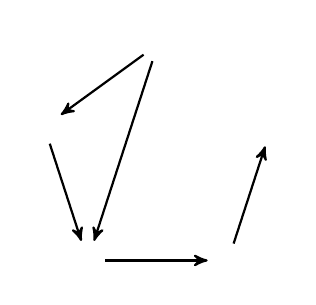
\begin{tikzpicture}[->,>=stealth',shorten >=1pt,auto,thick,main
	  node/.style={circle,fill=black,draw,font=\sffamily\Large\bfseries,inner
	  sep=0pt, minimum width=4pt}]
	
	  \node[regular polygon, regular polygon sides=5, minimum
	  size=3cm,name=x,fill=white, draw=none] at (0,0) {}; 
	  \foreach \corner in {1,2,...,5}
	  	  \ifthenelse{\equal{\corner}{1}}{
			\node[fill=white,circle,minimum width=12pt] (\corner) at (x.corner \corner){}
	  	  	}{
			\node[circle,minimum width=12pt] (\corner) at (x.corner \corner){}
	  	  	};
	
	  \path[every node/.style={font=\sffamily\small}]
	    (1) edge node {} (2)
	    (2) edge node {} (3)
	    (3) edge node {} (4)
	    (4) edge node {} (5)
	
	    (1) edge node {} (3)
	  ;
	\end{tikzpicture}
	\hspace{3mm}
	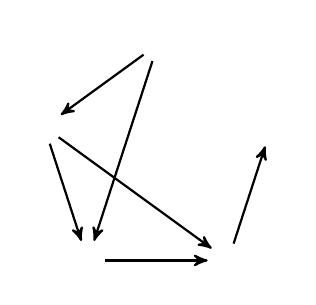
\begin{tikzpicture}[->,>=stealth',shorten >=1pt,auto,node distance=3cm,
	  thick,main
	  node/.style={circle,fill=white,draw,font=\sffamily\Large\bfseries,inner
	  sep=0pt, minimum width=4pt}]
	
	  \node[regular polygon, regular polygon sides=5, minimum
	  size=3cm,name=x,fill=white, draw=none] at (0,0) {}; 
	  \foreach \corner in {1,2,...,5}
	  	  \ifthenelse{\equal{\corner}{1}}{
			\node[fill=white,circle,minimum width=12pt] (\corner) at (x.corner \corner){}
	  	  	}{
			\node[circle,minimum width=12pt] (\corner) at (x.corner \corner){}
	  	  	};
	
	  \path[every node/.style={font=\sffamily\small}]
	    (1) edge node {} (2)
	    (2) edge node {} (3)
	    (3) edge node {} (4)
	    (4) edge node {} (5)
	
	    (1) edge node {} (3)
	    (2) edge node {} (4)
	  ;
	        
	\end{tikzpicture}
	\hspace{3mm}
	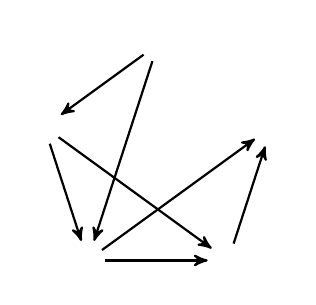
\begin{tikzpicture}[->,>=stealth',shorten >=1pt,auto,node distance=3cm,
	  thick,main
	  node/.style={circle,fill=black,draw,font=\sffamily\Large\bfseries,inner
	  sep=0pt, minimum width=4pt}]
	
	  \node[regular polygon, regular polygon sides=5, minimum
	  size=3cm,name=x,fill=white, draw=none] at (0,0) {}; 
	  \foreach \corner in {1,2,...,5}
	  	  \ifthenelse{\equal{\corner}{1}}{
			\node[fill=white,circle,minimum width=12pt] (\corner) at (x.corner \corner){}
	  	  	}{
			\node[circle,minimum width=12pt] (\corner) at (x.corner \corner){}
	  	  	};
	
	  \path[every node/.style={font=\sffamily\small}]
	    (1) edge node {} (2)
	    (2) edge node {} (3)
	    (3) edge node {} (4)
	    (4) edge node {} (5)
	    (1) edge node {} (3)
	    (2) edge node {} (4)
	    (3) edge node {} (5)
	  ;
	  
	  
	\end{tikzpicture}
	\caption{\codeCap{Refs} patterns}
	\label{fig:aserefs}
\end{figure}



\subsubsection{\code{Params} and \code{ParamCircle} Query Series for the
\code{numParameters} Metric} Two series of queries were constructed for this
metric, because of performance reasons. The \code{Params} query series is the more
complex and some tools exceed the time limit in the benchmark. The
\code{ParamsCircle} query series is a simplification of the \code{Params}
series.

The goal of this constructed query series is to create patterns with the same
body, but with an increasing number of parameters. The first of these queries
(returning one parameter) is shown in \figref{fig:aseparams}, where the
parameter is the blue object. Other queries use the same body, but add sen1,
then sen2, then other variables to the parameter list.

\begin{figure}[Htb]
\begin{center}
    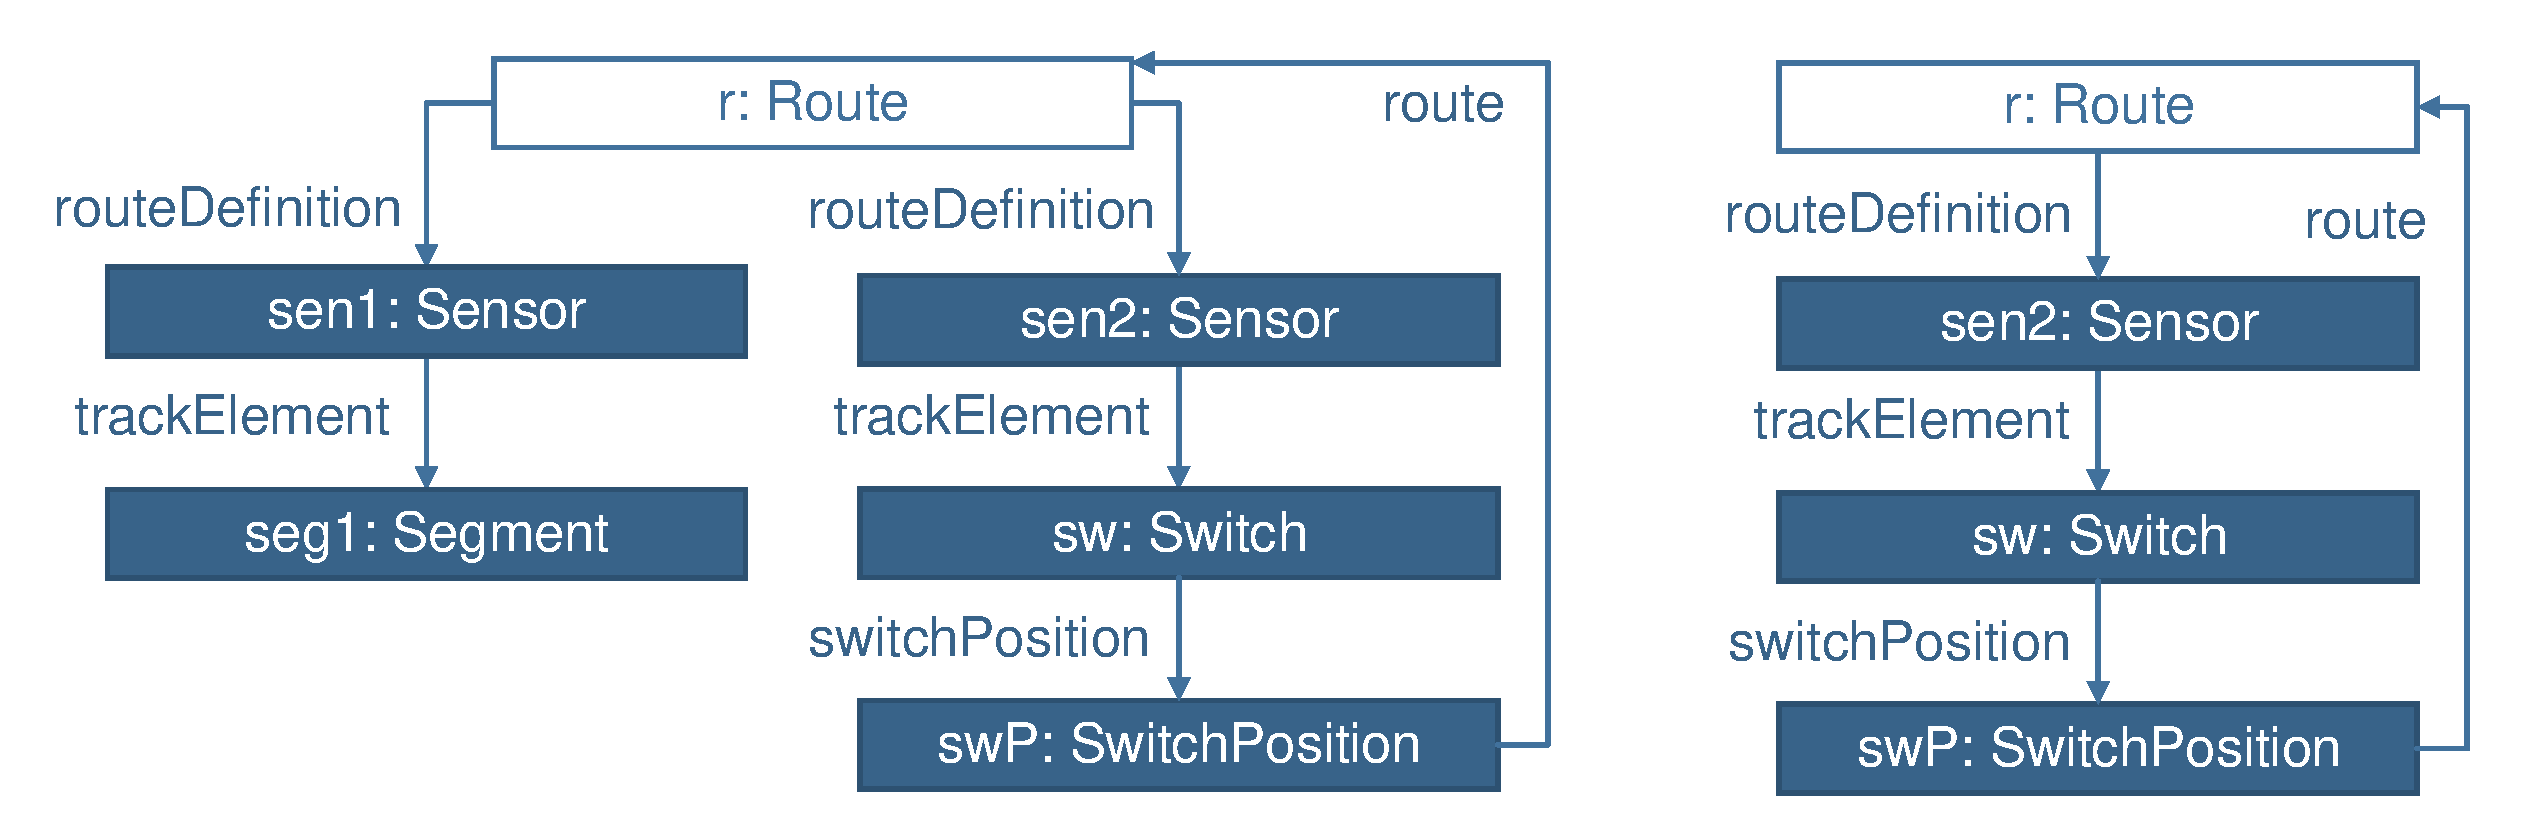
\includegraphics[scale=0.4]{figures/parameters.pdf}
    \caption{The \codeCap{Params} and \codeCap{ParamsCircle} pattern schemas (first step).}
    \label{fig:aseparams}
\end{center}
\end{figure}



\subsubsection{\code{Checks} Query Series for the \code{numAttrChecks} Metric}
Each \code{Checks} query use the same pattern body described by the pattern
schema in \figref{fig:asechecks}, but each one is extended with an increasing
number of attribute check constraints. These check constraints filter results
based on the \emph{year, height} and \emph{length} value of the segments \emph{seg1} and
\emph{seg2}, resulting in seven queries.

\begin{figure}[Htb]
\begin{center}
    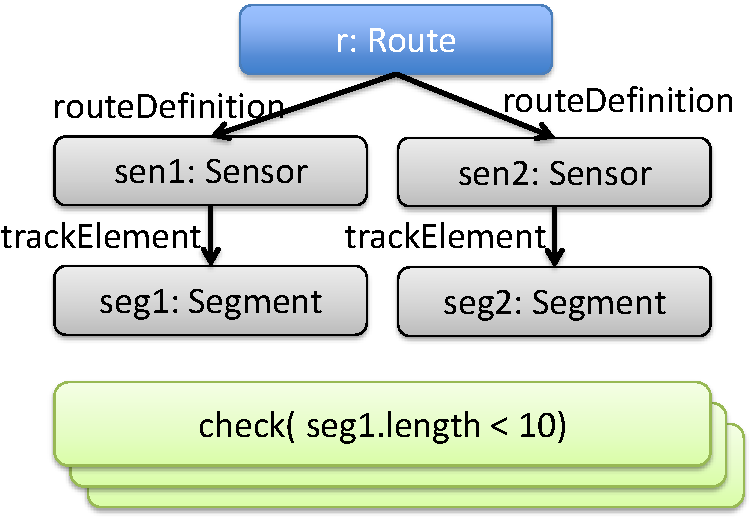
\includegraphics[scale=0.4]{figures/checks.pdf}
    \caption{The \codeCap{Checks} pattern schema.}
    \label{fig:asechecks}
\end{center}
\end{figure}


\subsubsection{\code{Negs} Query Series for the \code{nestedNacDepth} Metric}
\code{Negs} queries present increasing number of nested \emph{neg} constraints.
These queries are defined based on the following schema: at the bottom there is
a pattern checking for segments with length less than ten. Next, for each query
a new segment is matched, and the previous pattern is encapsulated in a negative
pattern call. $i=5$ queries are defined in the benchmark, described by the
schema in \figref{fig:asenegs}.

\begin{figure}[!ht]
\begin{center}
    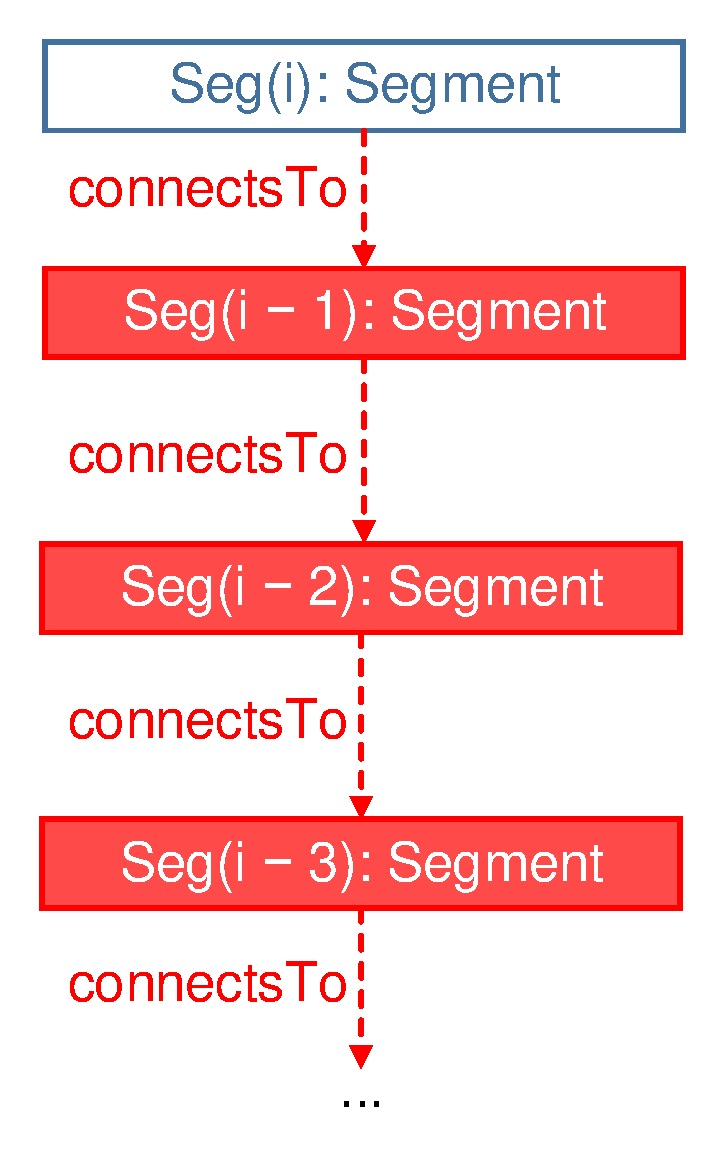
\includegraphics[scale=0.4]{figures/negs.pdf}
    \caption{The \codeCap{Negs} pattern schema.}
    \label{fig:asenegs}
\end{center}
\end{figure}

\begin{table}[Htb]
	\centering
	\footnotesize
	\begin{tabular}{|l|c|c|c|c|c|}
	\hline 
	\textbf{Query series} & \textbf{numParameters} & \textbf{numVariables} &
	\textbf{numEdgeConstraints} & \textbf{numAttrChecks} &
	\textbf{nestedNacDepth}\\ \hline Param & \cellcolor{blue!25}1--5 & 8 & 8 & 0 & 0\\ \hline ParamCircle & \cellcolor{blue!25}1--5 & 6 & 6 & 0 & 0\\ \hline
	Locals & 1 & \cellcolor{blue!25}3--7 & 6 & 0 & 0\\ \hline
	Refs & 1 & 5 & \cellcolor{blue!25}4--7 & 0 & 0\\ \hline
	Checks & 1 & 5--11 & 4--10 & \cellcolor{blue!25}0--6 & 0\\ \hline
	Neg & 2--6 & 3--11 & 1--5 & 1 & \cellcolor{blue!25}0--10\\ \hline
	\end{tabular}
	\caption{Query-only metrics.}
	\label{tab:queryonlymetrics}
\end{table}


After the construction of the query series, we evaluated the query only metrics
on them. \autoref{tab:queryonlymetrics} shows the results of the evaluation:
each cell contains the value or range of values that we got on each query
series. This table confirms that there are query series for every metric (shown
in blue), and each query series differ in one or more metrics.

\subsection{Complex Analysis}

\chapter{Train Benchmark Implementation}

\section{Original Version}

\subsection{Framework}

\begin{figure}[!Htb]
	\centering
	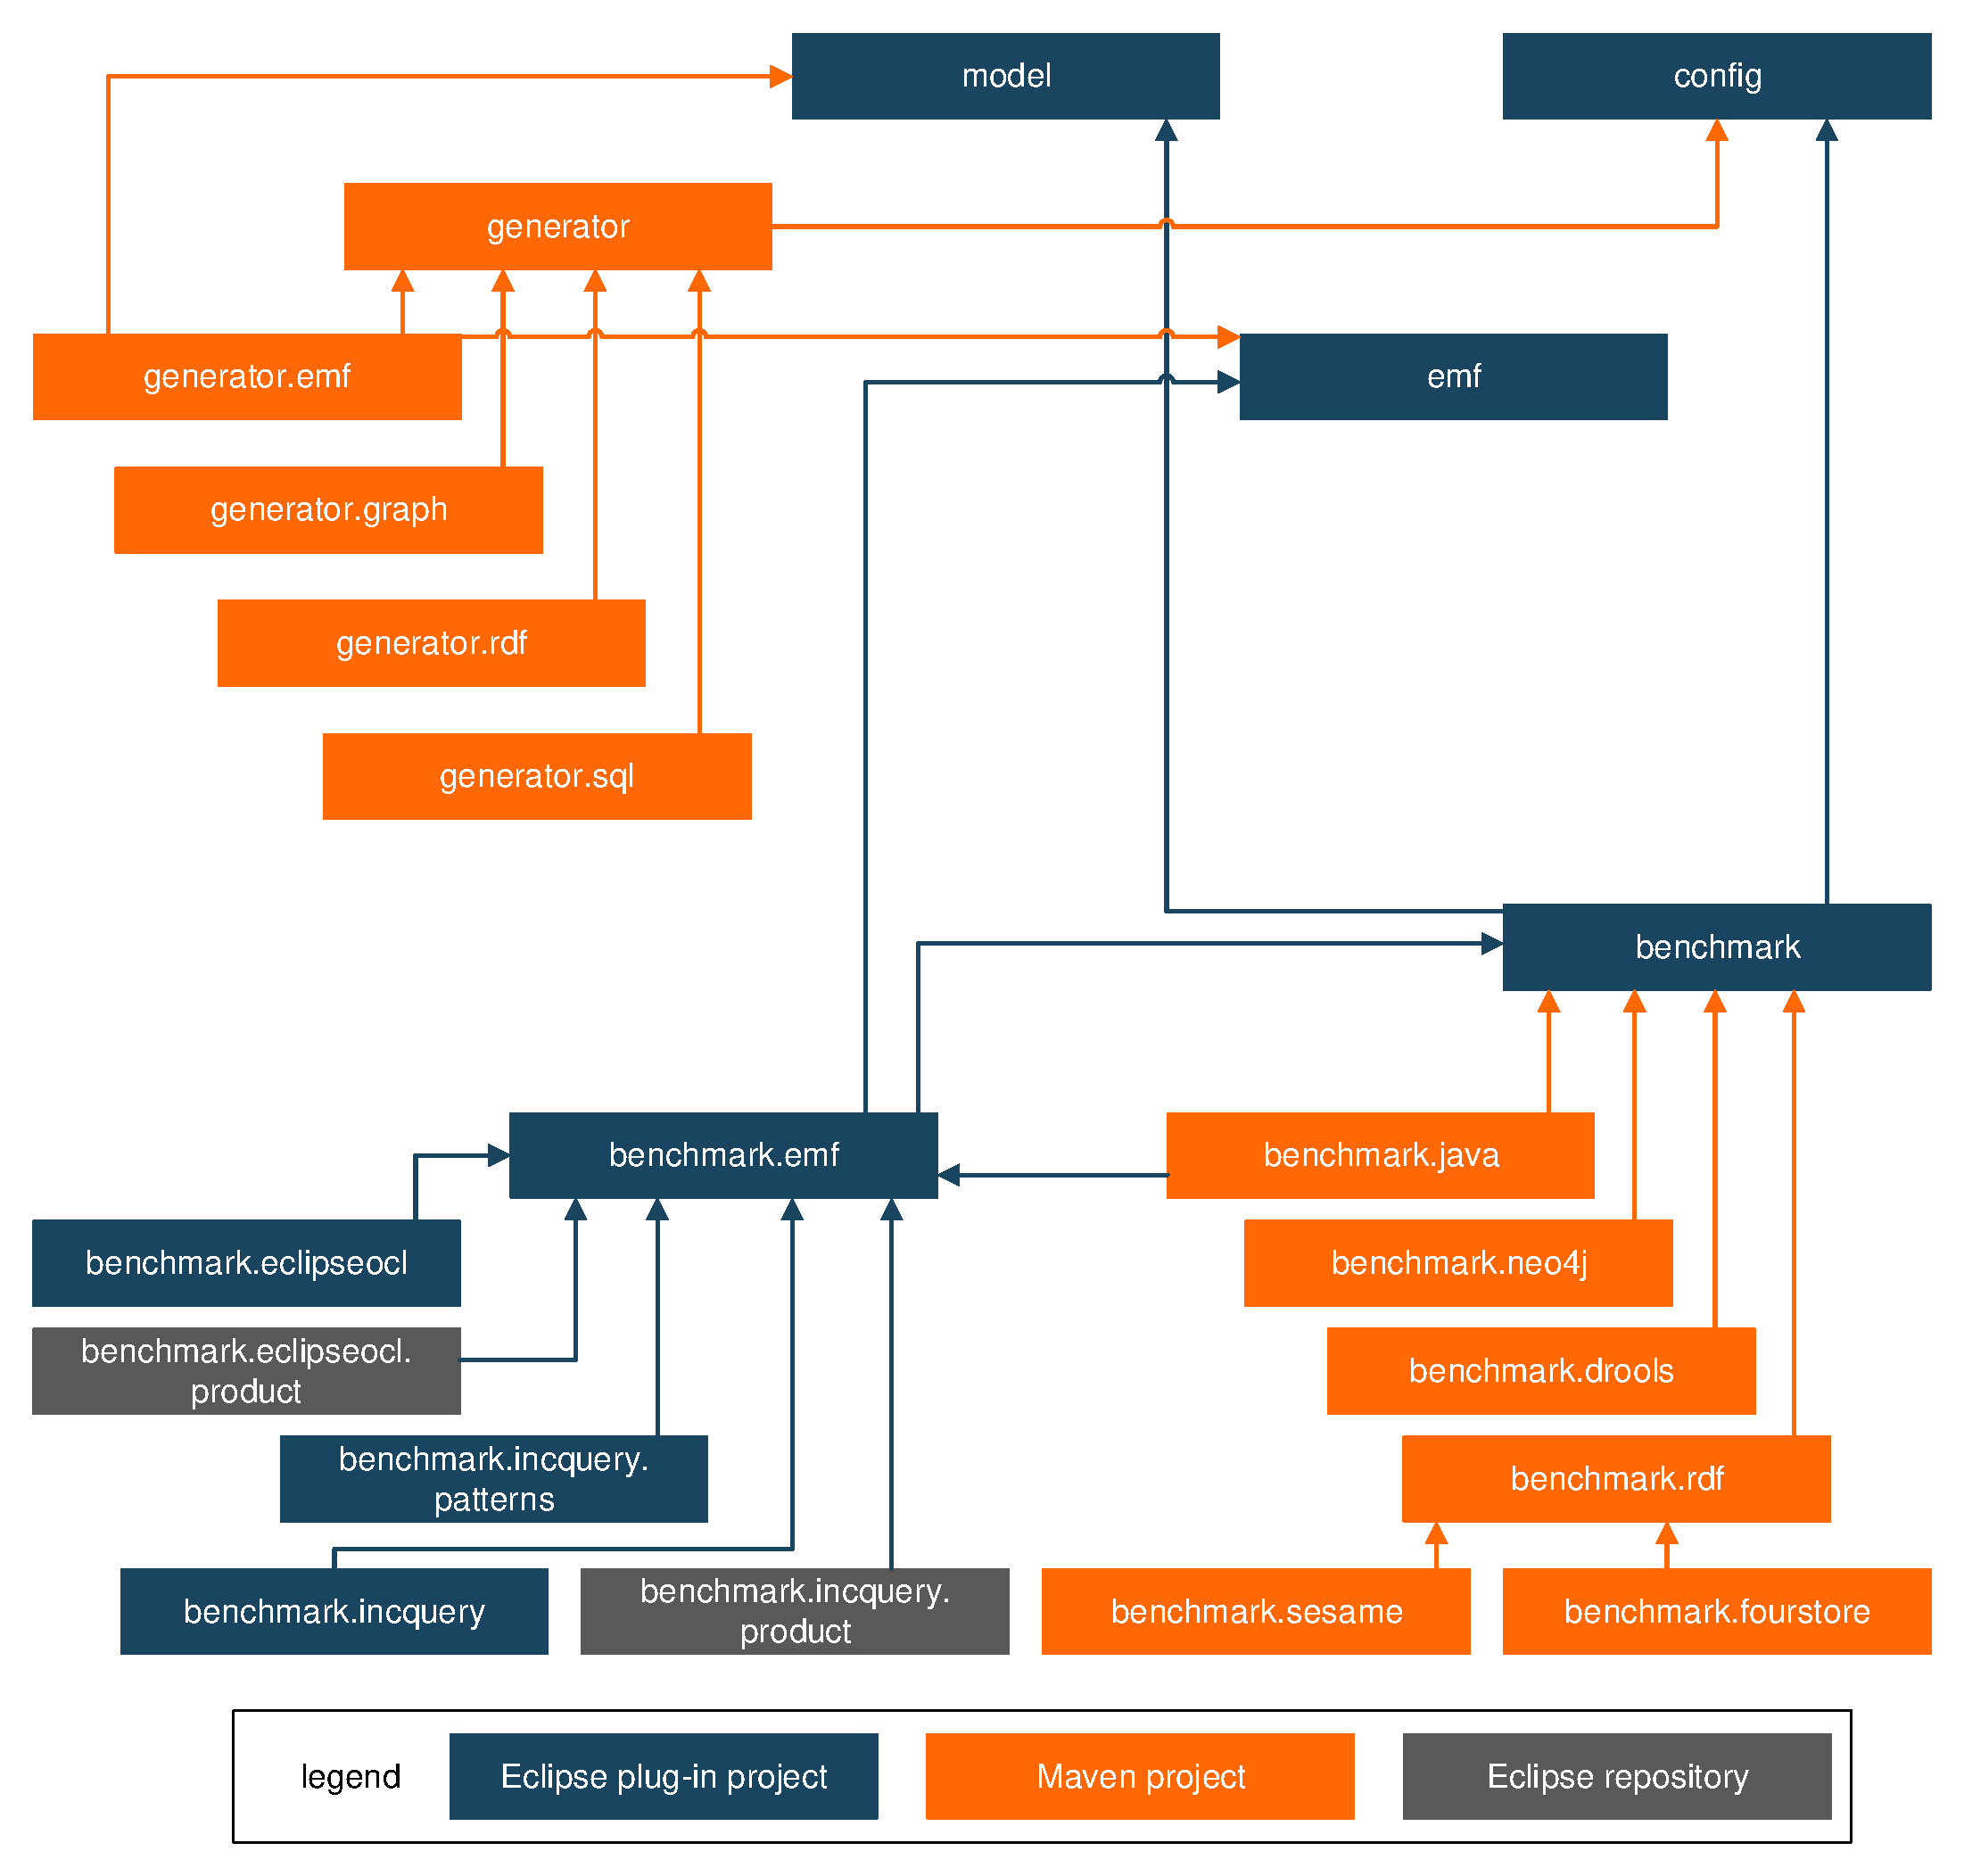
\includegraphics[width=\textwidth]{figures/trainbenchmark-modules}
	\caption{The Maven modules defined in the Train Benchmark. Note that artifact ids of the modules are abbreviated and their full id starts with \texttt{hu.bme.mit.trainbenchmark}.}
	\label{fig:trainbenchmark-modules}
\end{figure}

\subsection{Architecture}

For the integration of the Train Benchmark projects and their third party dependencies, we use Apache Maven~\cite{Maven}. The dependencies are shown in \figref{fig:trainbenchmark-modules}.

In this section, we briefly describe each module's tasks and responsibilities.

\subsubsection{Parent module}

The \texttt{hu.bme.mit.trainbenchmark} module is the parent module which contains the modules used in the Train Benchmark. Building this Maven module builds all child modules as well.

\subsubsection{Central modules}

The \texttt{hu.bme.mit.trainbenchmark.model} module contains the reference metamodel represented in EMF.

The \texttt{hu.bme.mit.trainbenchmark.config} module contains classes and constants used by the \emph{generator} and the \emph{benchmark} projects.



\subsubsection{Representation-specific modules}

The \texttt{hu.bme.mit.trainbenchmark.emf} and \texttt{hu.bme.mit.trainbenchmark.rdf} modules contain classes and constants used by the particular representations.



\subsubsection{Generator modules}

The \texttt{hu.bme.mit.trainbenchmark.generator.*} modules are responsible for generating the instance models for the benchmarks.

\begin{itemize}
  \item \texttt{emf}: generates an EMF instance model.
  \item \texttt{graph}: generates a property graph model in the specified format: GraphML (default), Blueprints GraphSON, Faunus GraphSON.
  \item \texttt{rdf}: generates an RDF instance model.
  \item \texttt{sql}: generates an SQL script which creates and loads the appropriate database tables.
\end{itemize}



\subsubsection{Benchmark modules}

The \texttt{hu.bme.mit.trainbenchmark.benchmark.*} modules are responsible for benchmarking. For the list of current implementations, see \ref{tools}.


\subsection{Services}

\subsection{API}

\subsection{time meas}

To obtain faithful execution times, we implemented a benchmarking framework,
which accounted for the time measurements with nanosecond precision (however, the accuracy may be lower than that),
 and the clear separation of phases enforced by the defined
interfaces. These model loading and querying functions were implemented using
functionally equivalent calls of a given tool. See Table~\ref{table:tools} for
the model management format and query language of the benchmarked tools. The
benchmarks were realized as Java applications.

\subsection{memory meas}
Before acquiring memory usage (free heap space) from the JVM, GC calls were triggered five times to sweep unfreed objects from the RAM.

\todo{+init +destroy, getmemusage, getbmr, \ldots}
Before every test
there is an unmeasured initialization phase. Environment initialization
instructions are executed, like clearing the OS file cache, triggering the
execution of the garbage collector, and starting server processes outside the
JVM if necessary (for example the Virtuoso server). At the end of each benchmark
in a separate unmeasured phase memory usage is measured (after calling the GC),
and finally network connections are closed, data structures are disposed, and
separate server processes are stopped.


\section{Discussion of fairness considerations}
Many different tools are measured in the benchmark which have various strenghts
and weaknesses. Model and query description languages have different expressive
power, however the benchmarking data model and queries are expressible in all
languages: executing them they return the correct number of invalid elements,
and semantically they are mapped as closely as languages enable, without using
cumbersome, unnatural expressions in a language.

EMF provides a class diagram like metamodel description language. Objects are
classified into classes, and connections between them are described by relations
(or attributes, when the target object's type is not a class, but a primitive
type, e.g. EInt). Enumerations, generalizations between classes, inverse
relations and simple cardinality restrictions are supported. Flat containment
hierarcy is used: a special class instance is created as the root object which can
hold all individuals. On the instance level EMF objects and instance relations
are created between them as described in \secref{sec:instanceGeneration}.

In ontologies, the OWL2 language supports all constructs that can be expressed in
EMF, thus the EMF metamodel is mapped to OWL2 TBox. The mapping is done by hand as
described in Sec. 16 of \cite{OMG2009ODM}. Ontology instance model elements are
generated equivalently to the EMF objects. Since an OWL2 file can be serialized
into RDF/XML, the same file is used as input for RDF databases and OWL
reasoners.

Neo4j defines a vertex-attributed, edge-labeled graph structure for describing
models. Here instance objects can be mapped to graph nodes, and instance
relations to graph edges. Metamodel information can be introduced into the graph
as labels. Key-value labels of nodes describe their types, instance names or
value of attributes (like the length of a Segment). The type of an edge can be
given as a label. Initially the generated model is loaded from a GraphML file,
which is also in XML syntax, as RDF/XML or XMI for EMF.

For the SQL test a custom relational schema is created as metamodel. Instance
model elements are stored in records, while primitive type attributes as
attributes, and relations as joins between tables. The input is also a textual
file, but it is not in XML format, it consists of SQL insert commands.

Queries are formulated similarly for the benchmarked tools. Variables are used
to bind them to objects. Types of variables and relation types between two
variables are constrained. For integer checks special check/filter constraints
are used; while the absence of instance model structures are described with
negation in all languages.

\todo{Az alábbi bekezdésből jön implementációs feladat, vagy a threats to validity-ben kell róla valamit írni?}

Of course unique feature of tools or lack of language expressiveness is not
highlighted in the benchmark, in order to be able to compare them. For example,
object type constraints are prescribed in the query, where the language allowed.
However in Java and OCL they are omitted, since it would be strange to read
unnecessary \emph{instanceof} and \emph{oclIsKindOf} expressions. On the other
hand, Drools requires these constraints, as variables are bound based on the
class it belongs to, and relation constraints can be expressed with this given
information. While EMF and OWL supports cardinality constraints and inverse
relations, RDF/RDFS does not support it. The former is not tested in the
benchmark, and the latter can be worked around by switching the subject and
object variables in a SPARQL query.
The handling of types and subsumption hierarchies were crucial for the
benchmark, and fortunatelly it is supported by most languages, although
reasoning capabilities must be turned on for ontology tools to work with this
implicit information. Other extra strengths special for a given tool were not
used, like complex cardinality constraints or transitive closure axioms in
ontology, transitive closure of the IQPL query language, or high availability
modes of Neo4j.

% OCL: org.eclipse.ocl.ecore.source_3.2.0.v20120522-1637.jar/org/eclipse/ocl/opposites/


\begin{figure*}[Hht]
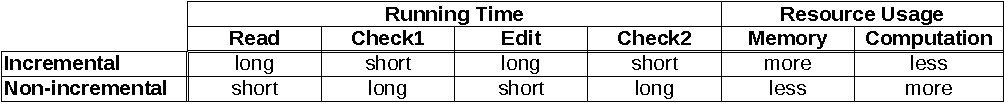
\includegraphics[width=2\columnwidth]{figures/incNonInc.pdf}
\caption{Incremental and non-incremental approaches}
\label{table:incNonInc}
\end{figure*}

Incremental and non-incremental engines use different computational approach,
which results in different characteristics as described by
\figref{table:incNonInc}. A clearly non-incremental tool does no extra work
during the load or modification of the model, but parses it into its memory, and
modifies the structure. In contrast an incremental tool usually builds some
auxiliary data structure (e.g. caches or indexes) on load, and maintains this
during modification (besides performing the modification) resulting in longer
running time. On the other hand incremental tools can return results quickly,
because they only read it from cache, or perform queries using the auxiliary
information (for fast access provided by indexes, utilize scope reduction or
rule reduction techniques). However, non-incremental tools must traverse the
whole model to search for invalid elements resulting in longer query answering
time. In conclusion, incremental tools usually needs less computation time when
the task is not batch dominated (i.e. there are no large transactions with rare
queries), while non-incremental tools need less memory (because there are no
auxiliary helper structures). This is why read+check1 and edit+check2 aggregated
values are used to compare all kind of tools.

Another differentiating factor can be query optimizaton. Formulating the same
constraint using different query primitives or different query ordering can
effect query performance highly. In the field of relational databases it has a
great literature used in tools (like MySQL, or the RDB backed Virtuoso), while
for graph query languages there are less research done in this field. 
\todo{cite needed} In the benchmark\ldots \todo{mit is kezdtünk vele\ldots}

\section{Questions to answer / Related work\ldots / Motivation (todo disassemble)}

\subsection{Why not existing benchmarks?}

There are already available benchmark definitions, however we created a new one
for measuring different tool capabilities. One of the most well known RDF
benchmark is the Berlin SPARQL Benchmark (BSBM) \cite{BerlinBenchmark}, which
models an e-commerce use-case. BSBM concentrates on throughput performance (in a
steady state) of parameterized queries, while our benchmark measures batch and
incremental query evaluation performance of fixed constraint checking queries.
The SP$^2$Bench \cite{SP2Bench} works on an unstructured dataset (DBLP) suited
for RDF data representation with the goal of measuring query evaluation
performance of SPARQL engines, concentrating on testing every feature of the
SPARQL language. In opposite, our benchmark queries a structured dataset, which
queries can be implemented in multiple query and data description languages.
Moreover, our benchmark scenarios address continous evolution of the dataset,
which is a future work in SP$^2$Bench, and also not addressed in \cite{SIB} and
\cite{DBpediaSparql}.

Other ontology benchmarks are the Lehigh University Benchmark (LUBM)
\cite{LUBMBenchmark}, and its improved version, the UOBM Ontology Benchmark
\cite{UOBM}. These are tailored for measuring reasoning capabilities of ontology
reasoners, while our goal is to compare query answering performaces.

Model transformation tools are compared annually in the Transformation Tool
Contest \cite{TTC} by solving model synchronisation, model execution and
simulation, verification use-cases from different application domains. The aim
is to compare expressiveness, usability and performance of different
tools in the field. \todo{kiegészíteni, +hivatkozás}

From the EMF domain we have not found general application benchmarks, or
comparison of EMF query technologies (like Eclipse OCL or EMF Query). However
there are performance measurements \cite{EMF-performance} about core EMF
functions, and different EMF configurations. We tried some relevant
configuration from these tips, but they were not effective, so we stuck at the
default EMF implementation.

We have not used relational database benchmarks, because the main scope of this
article are graph-based databases, and MySQL was included only for a rough
comparison. RDB benchmarks usually use relational schemas (and not graph-based
metamodels), and measure throughput with concurrent modifications like as
defined in the TPC-C \cite{tpc-c} benchmark.

Egyed published papers about verifying and fixing inconsistencies in UML models
\cite{Egyed-fixingInconsistencies, Egyed-instantConsistency} with performance
and memory consumption measurements \cite{Egyed-incConsistency} of the
UMLAnalyzer tool. They measured 19 rules and 30 independent UML models, scaling
up to $100 000$ elements. The tool evaluates OCL expressions in sub-millisecond
time using an impact analyzer approach.

Praxis \cite{falleri-praxis} use rule-reduction technique to provide incremental
instance model validation. It represents the model and edits using an operation
based approach. Technically Java, UML or Movida metamodels can be used, and
conforming instances as well as edit operations are translated to Prolog facts.
Constraints are represented as prolog rules, which are evaluated when they are
triggered based on the user written impact list. The paper reports evaluation
performance in the 0.1 second range (without measuring the conversion time), and
very low (below megabyte during evaluation, and tens of megabytes during
modification at maximum) memory usage.

To summarize, our benchmark concentrates to the model validation use-case, where
constraints (formulated as queries) are fixed, and instance models are evolving.
The benchmark measures the batch phase and incremental phases separately, and
evaluates them for multiple modeling domains (EMF, RDF, OWL, GDB, RDB).

% Social Network Intelligence Benchmark (SIB):
%   Olyan kérdéseket gyűjtöttek, ahol SPARQL jó. _Csak query_, throughput. (Ügyes SPARQL konstrukciók.)
% DBpedia SPARQL Benchmark:
%   Csak query, throughput. De real world.

\subsection{Why this specific domain?}
This domain is selected because it is small (contains only nine concepts), easy
to understand, and no deep domain knowledge is required. All queries can be
expressed over the described metamodel, and the railway terms suggest the field
of critical (or critical embedded) systems, where instance model validation is
used during the software development process.

\subsection{Why these instance models?}
Instance models are generated systematically from pre-defined blocks. This
reflects how large models of common design applications are built: domain
engineers connect modules with minimal variations, chosen from predefined
library elements. Large number of instance model elements can also be
auto-generated by a program, which connects building blocks created from
templates.

\subsection{Are these queries representative?}


% MORE threats : )
We tried to mitigate \emph{internal validity} threats by reducing the number of
uncontrolled variables during measurements: a physical machine was used with all
unnecessary software components turned off and every execution was isolated into
a freshly initialized JVM.

The queries are semantically equivalent in the different query languages and the
result sets are the same for every model. Additionally, to ensure comparable
results the created high-quality query implementations were reviewed: the OCL
implementation by Ed Willink from the Eclipse OCL project, the usage of Impact
Analyzer by Axel Uhl from the Impact Analyzer developer team. The graph patterns
were written by the developers of \incquery{}.

The metamodel and the query specifications were motivated by an industrial case
study, and the selected queries feature commonly used validation tasks such as
attribute and reference checks or cycle detection. We tried to ensure that the
instance models have a similar structure and distribution to other models by
parameterizing the generation process based on our experience with other
domains. To summarize, we believe that the train domain and the generated
instance models represent other domain-specific languages and available instance
models well.

Our current measurements only loaded and executed a single query in each run.
When loading multiple queries, query interference may change the results
greatly. A more detailed evaluation of this issue is planned for the future.

Considering resource-constrained environments, we believe that limiting
available memory will alter the results the most, as the memory management
overhead will reduce the performance of \incquery{}.

It is important to note that heap usage were measured after executing a garbage
collection, so these measurements do not contain memory usage of temporary
constructs. This means that maximum heap usage might have been larger. Furthermore,
limiting heap space by the maximum usage results in excessive garbage collection
and thus an increased runtime. However, in our experience setting the limit to
two times the measured values, such issues do not occur.

In case of the benchmark queries, we measured a $1.5$ GB heap size in case of a
model with $3.5$M model elements that we believe is manageable in a developer
machine with 4--8 GB of RAM. On the other hand, when handling such large
models the existing user interface itself could become a bottleneck. Thus we
believe, our measurement results hold also in the integrated development
environments.


\section{Extended Version}
\subsection{Framework}
\subsection{Architecture}
\subsection{Services}
\subsection{API}


\subsection{Implementation Details}

These query series are first defined in graph patterns and then formalized using
a query language suited for the given tool. The presented query series
were implemented using each model query technology mentioned in 
\autoref{sec:benchmark_overview}. In \figref{fig:patterns} the sample
implementation of the \code{locals\_3} query is depicted.

\begin{figure*}[tp]
\begin{center}
	\centering
    \begin{tabular}{c}
	    \begin{subfigure}[t]{0.38 
	    \textwidth}
	        \centering
	        {\alignListing
	                  \sourceIQPL{figures/queries/ase_locals_3.eiq}
	        }
	        \caption{\incquery{} graph pattern}
	        \label{fig:iqlocals3}
		\end{subfigure}
		
		\\
		
		%~ %add desired spacing between images, e. g. ~, \quad, \qquad etc. 
	    \begin{subfigure}[t]{0.38\textwidth}
	        \centering
	        {\alignListing
	                  \sourceSPARQL{figures/queries/ase_locals_3.sparql}
	        }
	        \caption{SPARQL graph pattern}
	        \label{fig:sparqllocals3}
		\end{subfigure}
	\end{tabular}
	~ %add desired spacing between images, e. g. ~, \quad, \qquad etc. 
    \begin{subfigure}[p]{0.56\textwidth}
        \centering
        {\alignListing
                  \sourceJava{figures/queries/ase_locals_3.java}
        }
        \caption{Java code}
        \label{fig:javalocals3}
	\end{subfigure}

  \caption{Pattern schemas for \codeCap{Locals\_3} query.}
  \label{fig:patterns}
\end{center} 
\end{figure*}
	
% \begin{figure*}[tp]
% \begin{center}
% 	\centering
%     \begin{tabular}{c}
% 	     \subfloat[\incquery{} pattern]
% 	     {\alignListing
% 		                  \sourceIQPL{../figures/queries/ase_locals_3.eiq}}
% 
% 			\\
% 
% 	     \subfloat[SPARQL pattern]
% 	     {\alignListing
% 	                   \sourceSPARQL{../figures/queries/ase_locals_3.sparql}}
% 	\end{tabular}
% 	~~~ %add desired spacing between images, e. g. ~, \quad, \qquad etc. 
%     \subfloat[Java code]
%     {\alignListing
%                   \sourceJava{../figures/queries/ase_locals_3.java}}\quad
%   \caption{Pattern schemas for \code{Locals_3} query}
%   \label{fig:patterns2}
% \end{center} 
% \end{figure*}
% 

In the IncQuery Pattern Language~\cite{IQlanguage} (\figref{fig:iqlocals3}), object constraints and reference constraints are used to describe the structure, and individuals matching the \code{Seg1} variable are returned.

Using the SPARQL~\cite{Sparql} notation (\figref{fig:sparqllocals3}), triples describe the same structural constraint, and the semantically equivalent query returns distinct matches of the \code{xSeg1} variable.

The query function was also coded in Java (illustrated in \figref{fig:javalocals3}). The model is traversed by embedded iterations and for every \code{Segment} the connections are checked. The implementation does not contain any search plan specific optimization (i.e.\ the embedding order of \code{for} cycles is ad-hoc), but it cuts unnecessary search branches at the earliest possibility.  This coding style represents an experienced programmer, who writes good quality source code. This way, such Java implementation could be used as a baseline in the future, to compare multiple tools qualitatively.


% [5/18/13 8:06:01 AM] Gábor Bergmann: On 5/18/13, at 7:27 AM, Ráth István wrote:
% > de nincs mögöttük ennél egy fokkal okosabb implementáció?
% a modell tulajdonságai (fokszámok, milyen élből mennyi van, stb.) alapján nem optimalizáltam, csak józan ésszel egymásba ágyazott ciklusokkal járom be
% [5/18/13 8:06:33 AM] Gábor Bergmann: persze ha le lehet vágni egy ágat (pl. mert adott paraméterekre már megvan egy illeszkedés), akkor igyekszem azonnal levágni

\section{Tools}

This benchmark was evaluated on three characteristically different query
technologies:
\begin{enumerate}
  \item An imperative \emph{local search-based} approach implemented completely in Java, operating on EMF models
  \item A declarative, \emph{incremental} approach based on the concepts of Rete networks as provided by the \incquery{} framework, operating on EMF models.
  \item A declarative, \emph{black-box} execution engine as implemented in the
  Sesame framework based on the SPARQL query specification language, operating on RDF models.
\end{enumerate}

Finally, we perform statistical correlation analysis against the
data set generated from the execution of our benchmarks and the evaluation of our
metrics.  



\chapter{Benchmark Results}


\section{Benchmarking Environment}
\label{sec:environment}

For the implementation details, source codes and raw results, see the benchmark website\footnote{\url{https://incquery.net/publications/trainbenchmark}}. In this section we describe the runtime environment, and highlight some design decisions.

The benchmark machine contains two dual-core Intel Xeon (3.00~GHz) CPU, 12~GBs of RAM and an SAS disk formatted to ext4 for storing the models. In order to alleviate disturbance of a running measurement and minimize noise in the results, a bare metal 64-bit Ubuntu 12.10 OS was installed with unnecessary services (like \texttt{cron}) turned off. Oracle JVM version 1.7.0\_51 is used as the Java environment and Eclipse Kepler Modeling 64-bit for Linux to satisfy specific tool dependencies.

The performance measurements of a tool was independent from the others, i.e.\ for every tool only its codebase was loaded, and every measurement of a scenario was started in a different JVM. Before the execution, the OS file cache was cleared, and swapping was disabled to avoid this kind of thrashing. Each test case (including all phases) must be run within a specified time limit (15 minutes), otherwise its process was killed.

Before acquiring memory usage (free heap space) from the JVM, GC calls were triggered five times to sweep unfreed objects from the RAM. For a JVM, 6~GB heap limit was specified.
%, and to compensate 64-bit pointers, OOPS (ordinary object pointers) compression was also turned on with the following options: (\code{-XX:MaxPermSize=256M -XX:+UseCompressedOops -Xmx25G}).

In the benchmark all cases were run 6 times, and the results were dumped into files, which were aggregated using the R statistical framework. The correlation results and performance plots are written into an HTML report.


\section{Tools}
\label{tools}
The measured tools generally work on graph-based models (like EMF~\cite{EMF} or RDF~\cite{RDF}), and provide a graph pattern-like query language. \autoref{tbl:tools} shows the list of current implementations.

\begin{table}[h]
	\centering
	\footnotesize
	\begin{tabular}{  | l | r | l | m{1.4cm} | c | >{\centering}m{1.9cm} | m{2.3cm} | }
	\hline
	\multicolumn{1}{|c|}{\bf Tool} & 
	\multicolumn{1}{c|}{\bf Version} & 
	\multicolumn{1}{c|}{\bf Model DL} & 
	\bf Query language & 
	\multicolumn{1}{c|}{\bf Incremental} & 
	\bf In-memory only & 
	\bf Implementation language \\ \hline 
	Java & 7.0 & EMF & Java & \ding{109} & \ding{108} & C++ \\ \hline
	Eclipse OCL & 3.3.0 & EMF & OCL & \ding{109} & \ding{108} & Java \\ \hline
	%OCL Impact Analyzer & 3.1.0 & EMF & OCL & \ding{108} & \ding{108} & Java \\ \hline
	\eiq{} & 0.7.2 & EMF & IQPL & \ding{108} & \ding{108} & Java \\ \hline
	Drools & 5.4.0 & EMF & DRL & \ding{108} & \ding{108} & Java \\ \hline
	Sesame & 2.7.9 & RDF & SPARQL & \ding{109} & \ding{108} & Java \\ \hline
	4store & 1.1.5 & RDF & SPARQL & \ding{109} & \ding{109} & C \\ \hline
	Neo4j & 1.9.2 & Graph & Cypher & \ding{109} & \ding{109} & Java \\ \hline
	\end{tabular}
	\caption{Tools used in the benchmark.}
	\label{tbl:tools}
\end{table}


\subsection{EMF-based Tools}

\subsubsection{Java}
An imperative \emph{local search-based} approach was implemented in Java, operating on \emph{Eclipse Modeling Framework (EMF)}~\cite{EMF} models. Queries are implemented as Java functions, traversing a model without any search plan optimization, but they cut unnecessary search branches at the earliest possibility.

\subsubsection{Eclipse OCL}

The OCL~\cite{OCL} language is commonly used for querying EMF model instances in validation frameworks. It is a standardized navigation-based query language, applicable over a range of modeling formalisms. Taking advantage of the expressive features and wide-spread adoption of this query language, the project Eclipse OCL~\cite{EclipseOCL} provides a powerful query interface that evaluates such expressions over EMF models.

%\subsection{OCL Impact Analyzer}
%The Eclipse OCL project also supports incremental evaluation by including an Impact Analyzer (IA)~\cite{ocl-ia2} that calculates the constraints to be reevaluated based on a model change. During EMF modifications it looks for possible context objects that could change the match set, and re-evaluation can be executed only for those objects. As it is intended only for incremental use, basic Eclipse OCL is used for calculating the first result set (batch mode).

\subsubsection{\eiq{}}
\eiq{}~\cite{models10} is an Eclipse Modeling project that provides incremental query evaluation using Rete~\cite{rete} nets. Queries can be written in its graph pattern based query language (IncQuery Pattern Language, IQPL~\cite{iqpl}), which is evaluated over EMF models.

\subsubsection{Drools}
Incremental query evaluation is also supported by the \concept{Drools}~\cite{Drools} rule engine developed by Red Hat. It is based on a variant of Rete~\cite{rete} (object-oriented Rete). Queries can be formalized using its own rule description language. Queries can be constructed by naming the ''when'' part of rules and acquiring their matches. While Drools is not an EMF tool per se, the Drools implementation of the \tb{} works on EMF models.


\subsection{RDF-based Tools}

\subsubsection{Sesame}
Sesame gives an API specification for many tools, and also provides its own implementation. The tool evaluates queries over RDF that are formulated as SPARQL~\cite{Sparql} graph patterns.

\subsubsection{4store}
4store~\cite{harris20094store} is an open source, distributed triplestore implemented in C. The main goal of 4store is to provide a high performance storage and query engine for semantic web applications. 

\subsubsection{\iqd}
\iqd{}~\cite{Izso:2013:IIG:2487766.2487772} is a distributed incremental graph query engine developed in the Budapest University of Technology and Economics. The goal of \iqd{} is to provide a scalable query engine by using a cluster of servers instead of a single workstation.


\subsection{Graph-based Tools}

\subsubsection{Neo4j}
As part of the NoSQL movement, database management systems emerged with a focus on graph storage and processing. As of 2014, the most popular graph database is 
Neo4j~\cite{neo4j}. The data model is based on graphs, where any node or edge can be labeled. Cypher can be used to query labeled graphs using its own graph pattern notation. This engine also uses disk for data storing, so a RAM disk is created during the benchmark.

\section{Measurement Results for Performance Comparison}
\label{sec:results}

The measurement results of the benchmark are displayed below. These diagrams show the batch query performance, incremental evaluation time, and memory usage of each tools, for different model sizes. Additionally, the initial and the updated result set size is displayed under the model sizes for the batch and incremental queries, respectively.

\subsection{SQL-based Tools}

\subsubsection{MySQL}
MySQL~\cite{mysql} is one of the most well-known and widely used open-source relational database management systems.

\subsection{Batch Validation (User Scenario)}

\forallqueries{\benchmarkresult{User_ReadPCheck0_\n}{Batch validation times for the \textsf{\n} query in the \textsf{User} scenario.}}

\subsection{Batch Validation (XForm Scenario)}

\forallqueries{\benchmarkresult{XForm_ReadPCheck0_\n}{Batch validation times for the \textsf{\n} query in the \textsf{XForm} scenario.}}

\subsection{Revalidation (User Scenario)}

\forallqueries{\benchmarkresult{User_SumModifyPSumReCheck_\n}{Revalidation times for the \textsf{\n} query.}}

\subsection{Revalidation (XForm Scenario)}

\forallqueries{\benchmarkresult{XForm_SumModifyPSumReCheck_\n}{Revalidation times for the \textsf{\n} query in the \textsf{XForm} scenario.}}

\subsection{Total Time (User Scenario)}

\forallqueries{\benchmarkresult{User_SumTime_\n}{Total time for the \textsf{\n} query in the \textsf{User} scenario.}}

\subsection{Total Time (XForm Scenario)}

\forallqueries{\benchmarkresult{XForm_SumTime_\n}{Total time for the \textsf{\n} query in the \textsf{XForm} scenario.}}

\subsection{Memory Usage (User Scenario)}

\forallqueries{\benchmarkresult{User_Memory_\n}{Memory consumption of the \textsf{\n} query in the \textsf{User} scenario.}}

\subsection{Memory Usage (XForm Scenario)}

\forallqueries{\benchmarkresult{User_Memory_\n}{Memory consumption of the \textsf{\n} query in the \textsf{XForm} scenario.}}

\subsection{Series of Edit Times (User Scenario)}

\benchmarkresult{series_DetEdit_64_PosLength}{Series of edit times for the \textsf{PosLength} query in the \textsf{User} scenario.}
\benchmarkresult{series_DetEdit_16_RouteSensor}{Series of edit times for the \textsf{RouteSensor} query in the \textsf{User} scenario.}
\benchmarkresult{series_DetEdit_1_SignalNeighbor}{Series of edit times for the \textsf{SignalNeighbor} query in the \textsf{User} scenario.}
\benchmarkresult{series_DetEdit_128_SwitchSensor}{Series of edit times for the \textsf{SwitchSensor} query in the \textsf{User} scenario.}

\subsection{Series of Incremental Revalidation Times (User Scenario)}

\benchmarkresult{series_DetCheck_64_PosLength}{Series of incremental revalidation times for the \textsf{PosLength} query in the \textsf{User} scenario.}
\benchmarkresult{series_DetCheck_16_RouteSensor}{Series of incremental revalidation times for the \textsf{RouteSensor} query in the \textsf{User} scenario.}
\benchmarkresult{series_DetCheck_1_SignalNeighbor}{Series of incremental revalidation times for the \textsf{SignalNeighbor} query in the \textsf{User} scenario.}
\benchmarkresult{series_DetCheck_128_SwitchSensor}{Series of incremental revalidation times for the \textsf{SwitchSensor} query in the \textsf{User} scenario.}

\section{Experimental Evaluation}
\label{sec:eval}
% Baba, 5 columns
%     Setup (hw-sw environment, measurement and data collection details)
%     Results
%         Figures, tables: results 
%     Analysis
%     Comparison/contrast with other benchmarks, answers to RQs 
% 



\subsection{Method of Analysis}
Our long-term goal is providing a catalog of reliable benchmark data that,
based on metrics of the model and the queries, will allow the engineer to
extrapolate the expected performance characteristics of various query
technologies, which in turn will support making an informed decision on the
solution to apply. In scope of this paper, we attempt to provide a necessary
prerequisite with a narrower focus of investigation: finding out which model and
query metrics are useful for predicting the performance 
of the various tools, over a wide range of different queries and model
structures.

A given metric can only be a useful predictor of a certain performance indicator
of a certain tool if they are strongly correlated. Therefore our analysis
investigated correlations of metrics and performance indicators. Neither
previous experience nor current measurement data supported a linear relationship
between these variables; therefore we opted to abandon the commonly used Pearson
correlation coefficient that is associated with linear regression. We rely
instead on Kendall's $\tau$ %and Spearman's $\rho$
 rank correlation coefficient, ranging from $-1$ to $+1$; without assuming a
 linear model, $\tau$ characterises the degree to which it can be said that
 larger values of the metric correspond to larger values of the performance
 indicator.

Correlation coefficients may lead to incorrect conclusions if the sample of
models and queries is too small. Therefore, whenever measuring an absolute value
of $\tau$, we additionally conducted the associated statistical test
($\tau$-test) to decide whether the detected correlation between the variables
is statistically significant ($p < 0.001$). Note that any such statistical result
is conditional to the uniform sampling of the selected queries and models.


A limitation of the approach is that two strongly correlated variables (e.g.\ 
\code{countEdges} and \code{countTriples}) may show up as equally good
predictors, but in reality they can not be used as two independent signals for
predicting performance (as most triples in our models are edges). The simple
correlation-based analysis presented here is intended as preliminary feature
selection; we intend to follow up with redundancy-reducing feature selection
techniques such as mRMR~\cite{mRMR-1453511} that can take into account which
metrics convey independent information. Afterwards, predicting the best choice
of technology based on the metric values is a problem of multivariate regression
/ classification, for which we plan to employ advanced machine learning
techniques (e.g.\ ID3~\cite{ID3-quinlan-1986} decision trees or
MARS~\cite{MARS-MR1091842} regression model) in future work.

\begin{figure*}[tp]
\begin{center}

    \begin{tabular}{c c c}
	    \begin{subfigure}[t]{0.31\textwidth}\centering
	    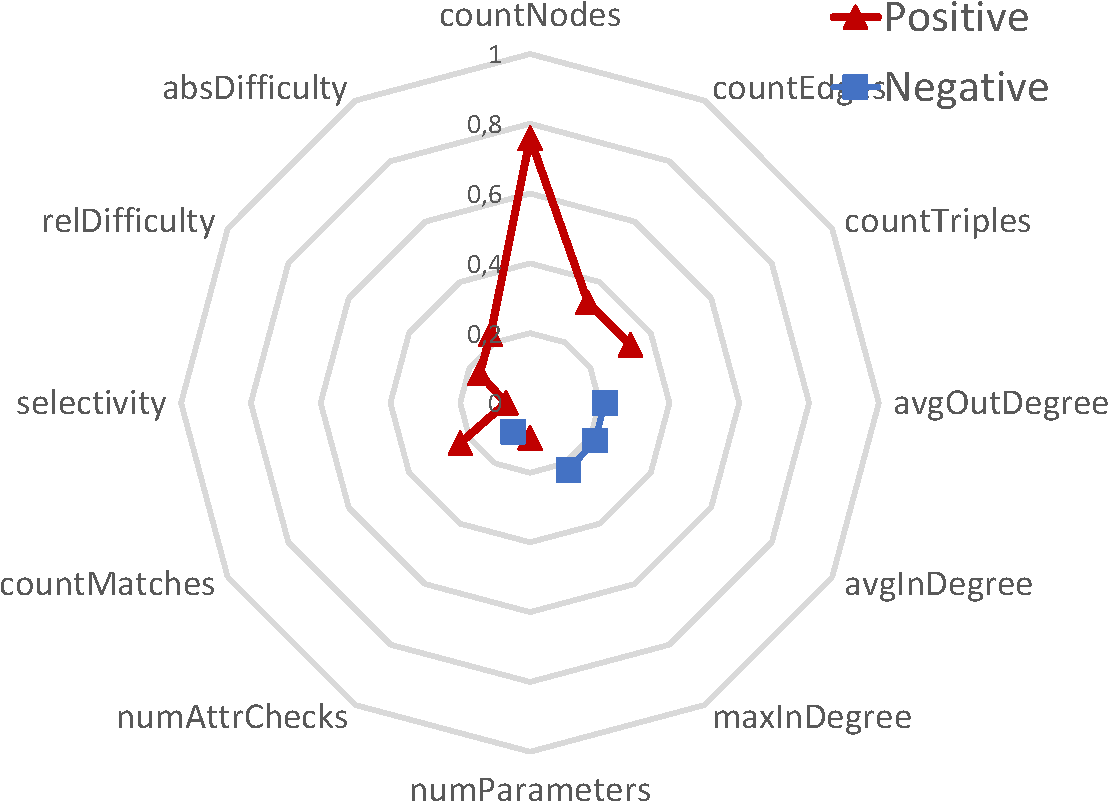
\includegraphics[width=0.95\textwidth]{figures/spider-java-memory.pdf}
	    \caption{Java Memory}\end{subfigure} &
	    \begin{subfigure}[t]{0.31\textwidth}\centering
	    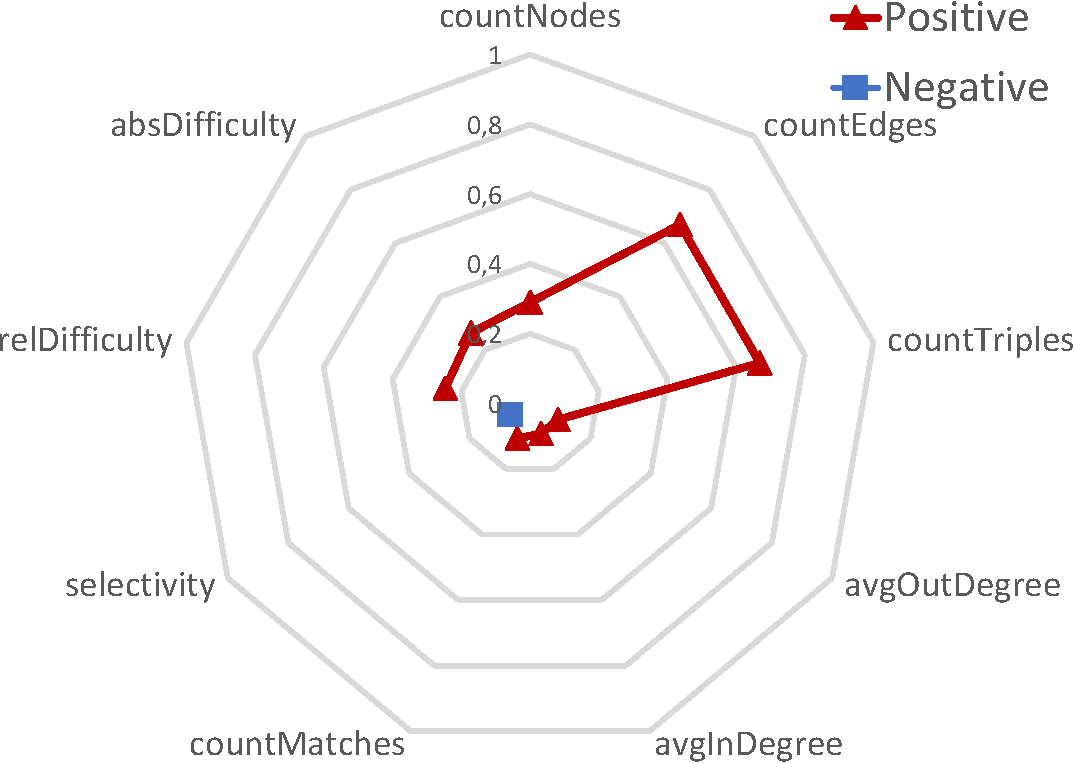
\includegraphics[width=0.95\textwidth]{figures/spider-java-read.pdf}
	    \caption{Java Read time}\end{subfigure} &
	    \begin{subfigure}[t]{0.31\textwidth}\centering
	    \includegraphics[width=0.95\textwidth]{figures/spider-java-check.pdf}
	    \caption{Java Check time}\end{subfigure} \\
	    \begin{subfigure}[t]{0.31\textwidth}\centering
	    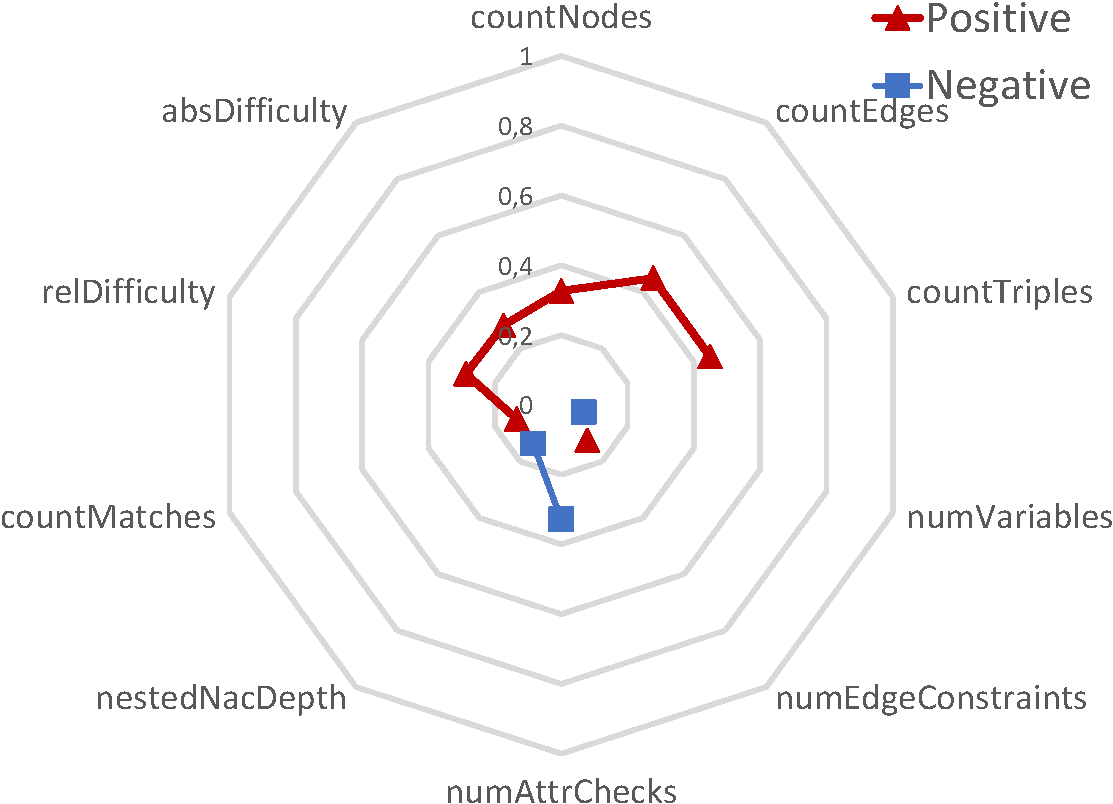
\includegraphics[width=0.95\textwidth]{figures/spider-iq-memory.pdf}
	    \caption{\incquery{} Memory}\end{subfigure} &
	    \begin{subfigure}[t]{0.31\textwidth}\centering
	    \includegraphics[width=0.95\textwidth]{figures/spider-iq-read.pdf}
	    \caption{\incquery{} Read time}\end{subfigure} &
	    \begin{subfigure}[t]{0.31\textwidth}\centering
	    \includegraphics[width=0.95\textwidth]{figures/spider-iq-check.pdf}
	    \caption{\incquery{} Check time}\end{subfigure} \\
	    \begin{subfigure}[t]{0.31\textwidth}\centering
	    \includegraphics[width=0.95\textwidth]{figures/spider-sesame-memory.pdf}
	    \caption{Sesame Memory}\end{subfigure} &
	    \begin{subfigure}[t]{0.31\textwidth}\centering
	    \includegraphics[width=0.95\textwidth]{figures/spider-sesame-read.pdf}
	    \caption{Sesame Read time}\end{subfigure} &
	    \begin{subfigure}[t]{0.31\textwidth}\centering
	    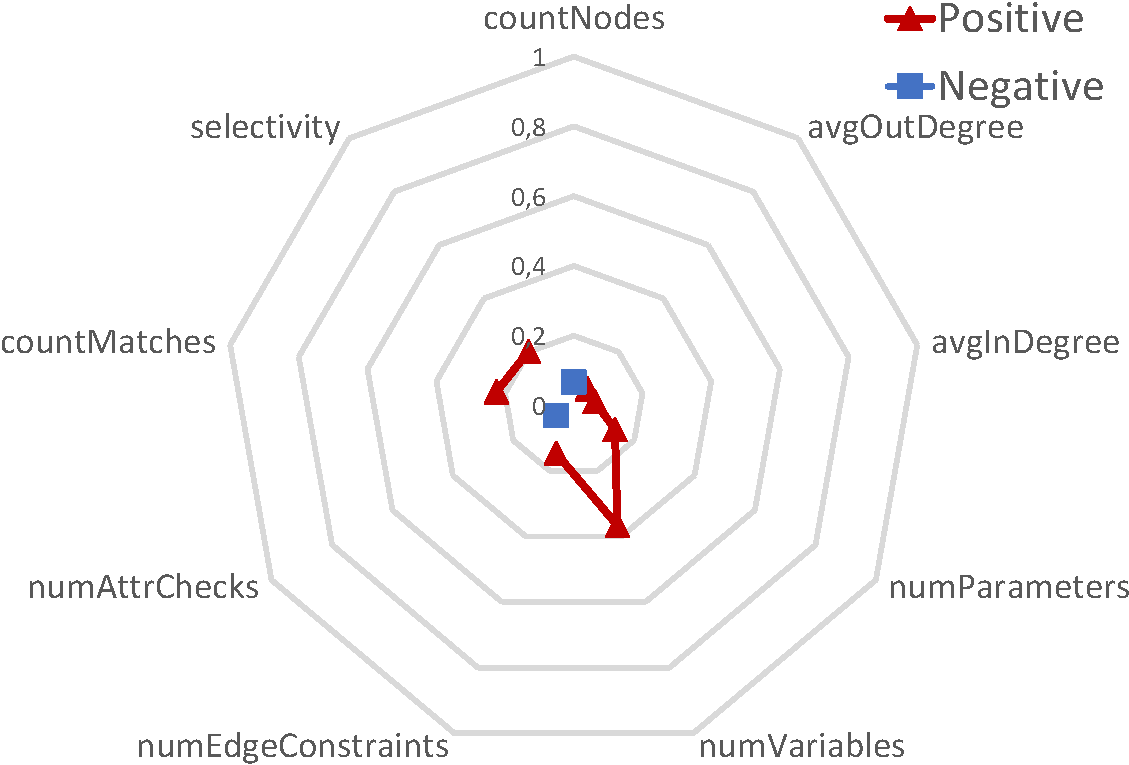
\includegraphics[width=0.95\textwidth]{figures/spider-sesame-check.pdf}
	    \caption{Sesame Check time}\end{subfigure} 
    \end{tabular}

  \caption{$\abs{\tau}$ of correlating ($p<0.001$) metrics for each performance indicator.}
  \label{fig:correlation-spider}
\end{center}
\end{figure*}

\subsection{Results}
For each tool performance indicator and each metric, we conducted Kendall's correlation test to see whether the data available is sufficient to form a statistically significant support of correlation between the performance indicator and the metric. For metrics that were found to correlate, the absolute value of Kendall's $\tau$ correlation coefficient is displayed on a spider chart specific to the performance indicator of the tool (see \autoref{fig:correlation-spider}); positive correlation values are displayed as red triangles, while negative ones as blue squares.  

\subsubsection{Evaluation}
Consistently with previously published results, the data shows that model size is a strong predictor of both model loading time and memory consumption, regardless of the technology.
\paragraph{Tool-specific Observations}
However, check times show a more diverse picture. The check times for the Java implementation (being a dominantly search-intensive approach) are additionally correlated with the query-on-model metrics as well, with the strongest correlation shown by the \emph{absDifficulty} metric. 

Interestingly, the best Sesame check time predictor turned out to be the number of pattern variables, and there is no significant correlation with any direct model metrics. 

Check times in \incquery{} are very strongly correlated to the number of matches -- which is to be expected of an incremental tool whose check phase consists of just enumerating the cached match set. As the incremental indexes are constructed during the load time, the model-on-query metrics become correlated with \incquery{} read time. It can also be highlighted that \incquery{} seems not to be sensitive towards the ``difficulty'' of the query (in any phase) or the model size (during the check phase) due to the very small correlations with corresponding metrics.
\paragraph{Metrics}
Overall, it can be said that model-only metrics are useful in predicting the performance of model persistence operations. However, query-based and combined metrics (such as our proposed \emph{abs-} and \emph{relDifficulty}) are necessary to provide a more thorough picture.
Note that since only statistically significant correlations are included, a low magnitude correlation does not necessarily mean a measurement error. It is possible that there is a true link between the two variables, but the $\tau$ value is lowered by other metrics that strongly influence the performance indicator. 
% \paragraph{Decision making}
% The Goal Question Metric (GQM) approach~\cite{gqm} can be used to make informed decisions about tool or language selection. A \emph{goal} can be that the processing of models must be efficient. \emph{Questions} would be: batch or incremental scenario is performed by the tools? How large is the model? What is the complexity of the queries? These can be answered using the relevant metrics of \figref{fig:correlation-spider}. Metrics with high correlation will have the most impact on runtime. In the future we plan to extend this benchmark, and build decision trees or more complex decision support systems that can aid domain engineers to choose the right tool and languages for their task.

% [5/18/13 8:29:53 AM] Varró, Daniel: Toolokról külön-külön kellene írni valamit
% [5/18/13 8:30:26 AM] Varró, Daniel: továbbá a végén arról, hogy a szakirodalomból ismert metrikák mennyire bizonyultak használhatónak vagy használhatatlannak
% [5/18/13 8:31:12 AM] Varró, Daniel: A negatív eredményeket / meglepetéseket is el kellene magyaráznunk, nemcsak a pozitív korrelációt

\subsubsection{Threats to Validity}
Regarding the technological foundations and methodology of our measurements, the
most important threats to validity stem from \emph{time measurement uncertainty}
and distortions due to transient effects such as \emph{garbage collection} in
the JVM and \emph{thrashing} due to heap size exhaustion. Such effects were
mitigated by using the most accurate Java time measurement method
(\code{System.nanoTime}), allocating as much heap as possible, and using a
timeout mechanism to identify and exclude cases affected by thrashing from the
results.
Additionally, it is also possible that there is sampling bias in our choice of
models and metrics; we believe that this is sufficiently mitigated by our
systematic choice of model generation strategies and the design principles of
the queries. To improve the magnitude of correlation we increased the sample
size by running the benchmarks ten times.
\chapter{Summary}

\appendix
\chapter{Appendix}
\label{appendix}

\section{Rete Networks for the Queries of the Train Benchmark}

The Rete algorithm uses \emph{tuples} to represent the vertices (along with their properties), edges and subgraphs in the graph. The algorithm defines an asynchronous network of communicating nodes. The Rete networks has three layers:

\begin{itemize}
  \item The top level consists of \emph{input nodes} which are type-instance indexers for the model. Each input node indexes a certain vertex type or edge label. The actual graph element is indicated by a vertex/edge icon in the upper right corner of the Rete node.
  \item \emph{Worker nodes} perform a transformation on the output of their parent node(s) and propagate the results. Partial query results are represented in tuples and stored in the memory of the worker node thus allowing for incremental query reevaluation.
  \item The bottom level consist of \emph{production nodes} which are terminators that provide an interface for fetching the results of the query and the changes introduced by the latest transformation.
\end{itemize}

In \figref{fig:rete-poslength-layout}--\figref{fig:rete-semaphoreneighbor-layout}, we present possible Rete networks layouts for the queries in the Train Benchmark.

\begin{figure}[htb]
\centering
\begin{minipage}[b]{0.4\textwidth}
\begin{center}
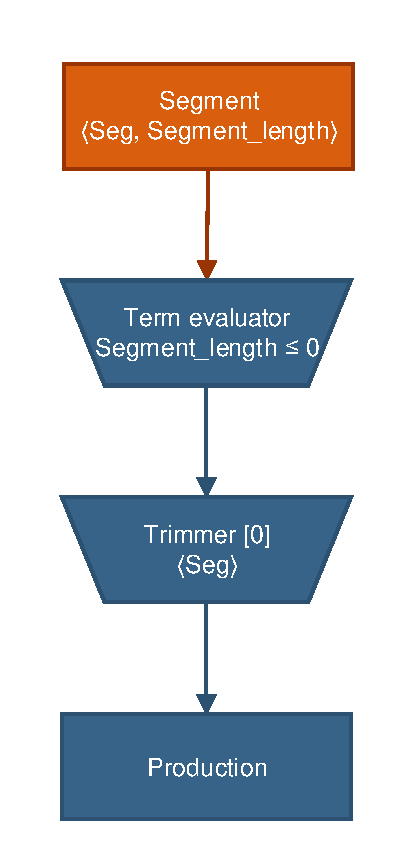
\includegraphics[scale=0.5]{figures/rete-poslength-layout.pdf}
\caption{The Rete network for the \textsf{PosLength} query.}
\label{fig:rete-poslength-layout}
\end{center}
\end{minipage}
\qquad
\begin{minipage}[b]{0.4\textwidth}
\begin{center}
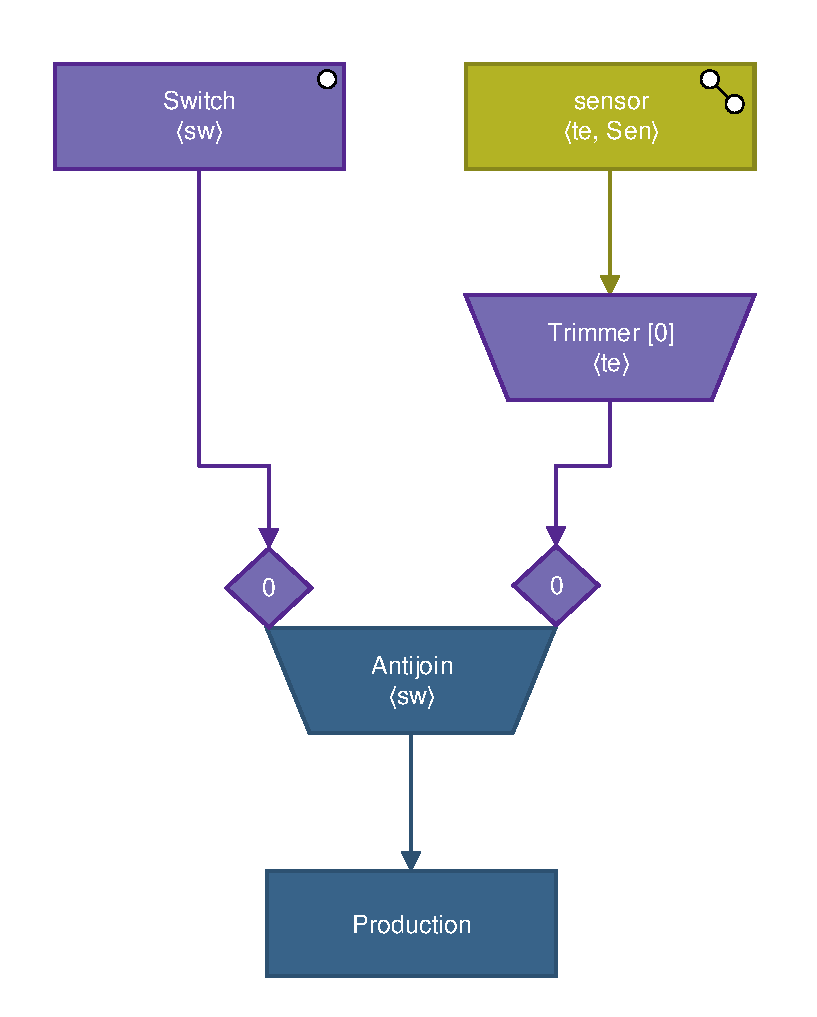
\includegraphics[scale=0.5]{figures/rete-switchsensor-layout.pdf}
\caption{The Rete network for the \textsf{SwitchSensor} query.}
\label{fig:rete-switchsensor-layout}
\end{center}
\end{minipage}
\end{figure}

%\begin{figure}[htb]
%\end{figure}

\begin{figure}[htb]
\begin{center}
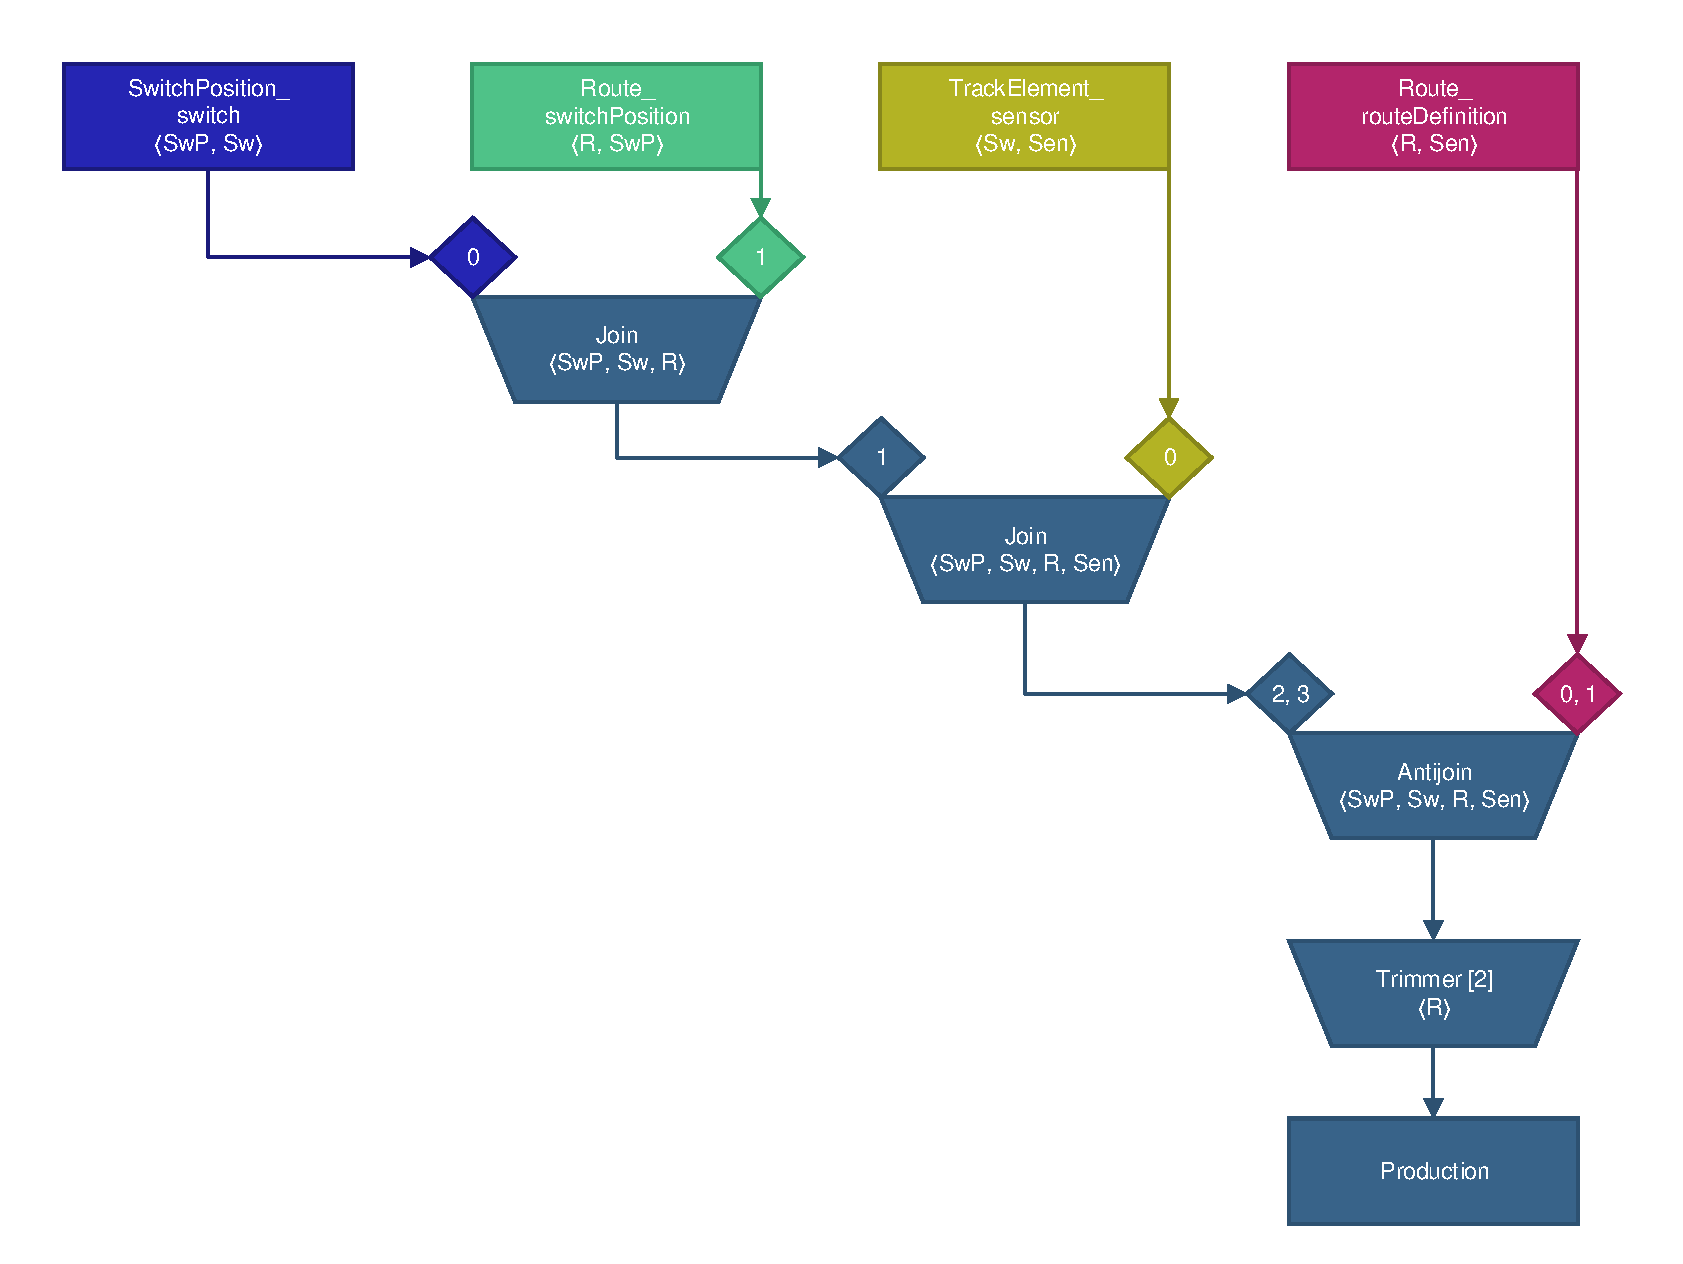
\includegraphics[scale=0.5]{figures/rete-routesensor-layout.pdf}
\caption{The Rete network for the \textsf{RouteSensor} query.}
\label{fig:rete-routesensor-layout}
\end{center}
\end{figure}

\begin{figure}[htb]
\begin{center}
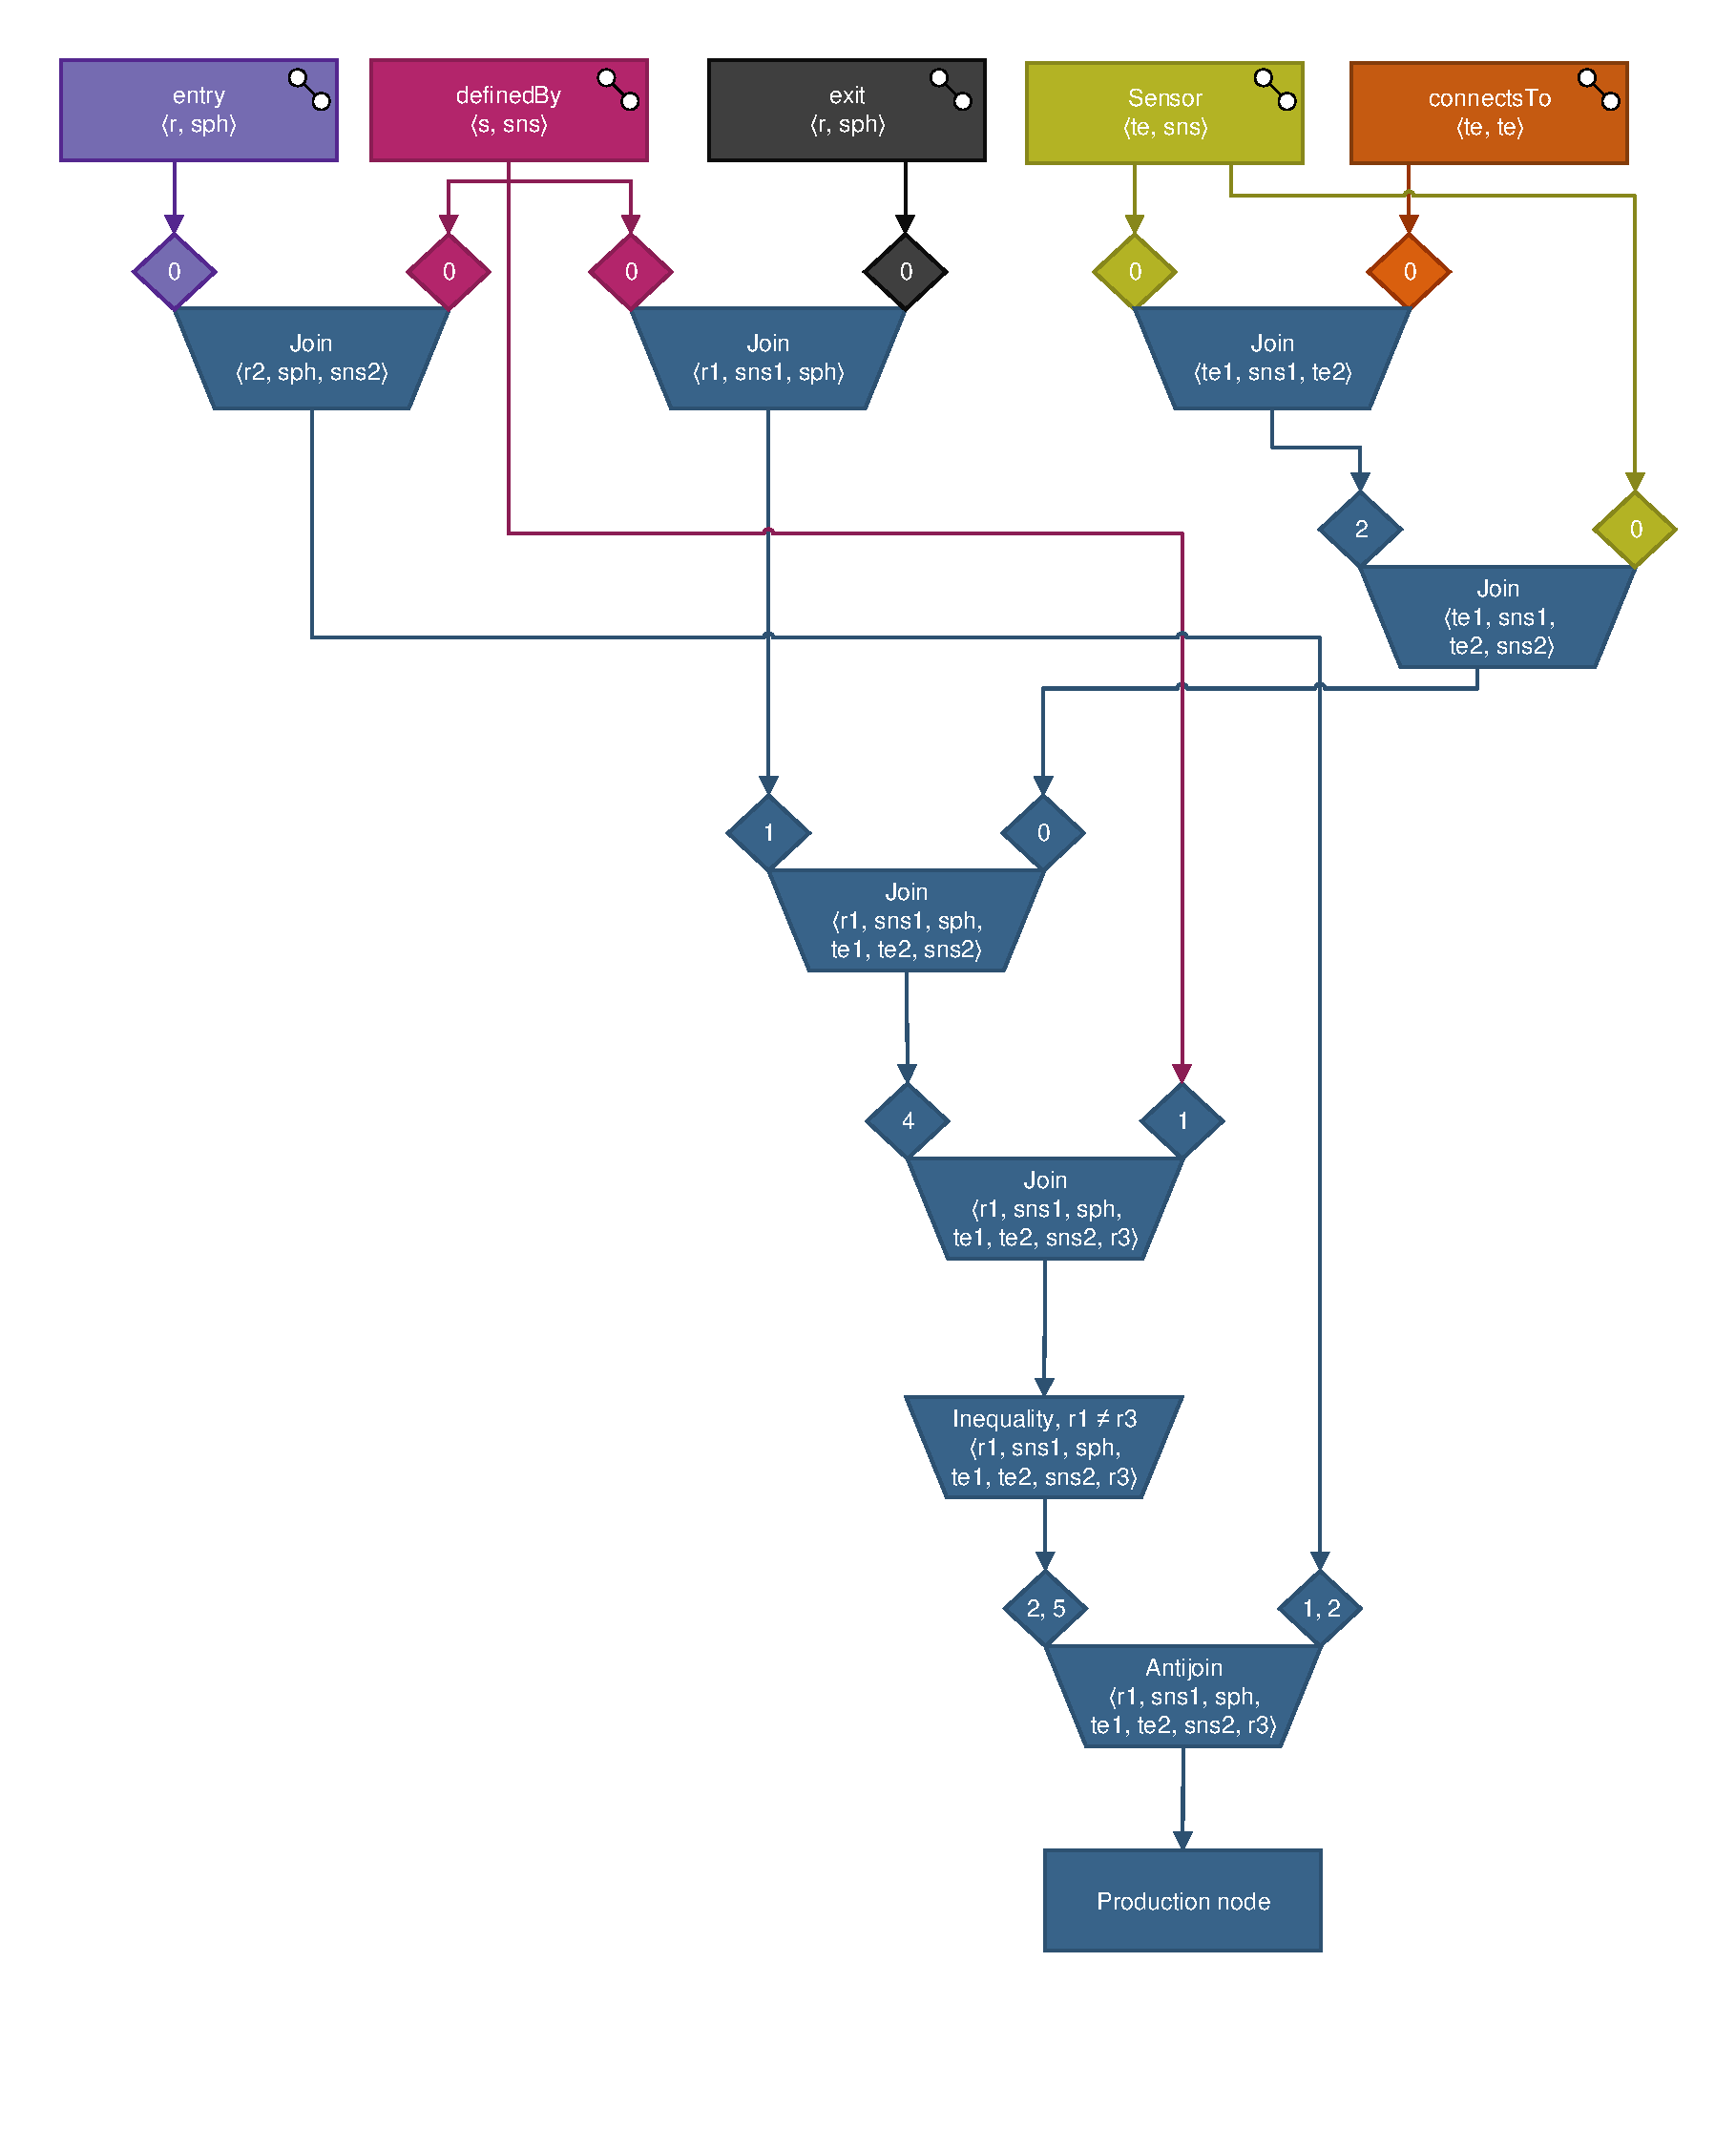
\includegraphics[scale=0.5]{figures/rete-semaphoreneighbor-layout.pdf}
\caption{The Rete network for the \textsf{SemaphoreNeighbor} query.}
\label{fig:rete-semaphoreneighbor-layout}
\end{center}
\end{figure}


\clearpage

\bibliographystyle{plain}
\bibliography{../bib/trainbenchmark,../bib/ase13}

\end{document}